% Estas slides tienen que abrirse con el programa pdfpc que soporta videos embebidos
% el comando es: pdfpc -g slides.pdf
% para los videos se requiere ubuntu-restricted-extras
% para la bibliografía se requiere biber y configurar texstudio

%\documentclass[compress,handout]{beamer}
\documentclass[aspectratio=169,compress]{beamer}

% add beamer preamble
% Theme customization
\setbeamertemplate{itemize item}[rectangle] % configure itemize
\setbeamertemplate{itemize subitem}[circle] % configure itemize
\setbeamertemplate{itemize subsubitem}[triangle] % configure itemize
\setbeamertemplate{navigation symbols}{} % remover simbolos de navegacion de las slides
\usefonttheme[onlymath]{serif} % simbolos matematicos en serif (Como es en latex original)
\setbeamersize{text margin left=3mm,text margin right=3mm} 

\setbeamertemplate{blocks}[rounded] % blocks corners rounded
\setbeamercolor{block body}{bg=blue!12,fg=black} % color of blocks
\setbeamertemplate{caption}{\raggedright\insertcaption\par} % elimina la palabra "Figura" del caption

\usepackage[overridenote]{pdfpc} % requires to download manually pdfpc.sty package from https://www.ctan.org/pkg/pdfpc

% add latex preamble
% para la bibliografía se requiere biber y configurar texstudio

% Latex packages
\usepackage[utf8]{inputenc}
\usepackage[T1]{fontenc} % para copiar acentos en español del pdf y permite acentos en las notas
\usepackage[spanish]{babel}
\usepackage[per-mode = symbol]{siunitx} % para manejar las unidades
\usepackage{multimedia} % to add videos with \movie command
\usepackage{multirow}
\usepackage{graphicx}
\usepackage{xcolor}
\usepackage{amsmath} % bmatrix
\usepackage[makeroom]{cancel} % \cancel to cancel terms in math equations
\renewcommand{\CancelColor}{\color{red}} % set red color for \cancel command
\usepackage[caption=false]{subfig} % caption = false elimina la palabra "Figura" del caption
\usepackage{import} % para el comando import (se usa para pdf_tex)
\captionsetup[subfigure]{labelformat=empty} % remover el indice del caption de la subfigura
\usepackage{booktabs} % \toprule \midrule \bottomrule
\usepackage[backend=biber]{biblatex} % set biber to format references. Must configure Biber in Texstudio
\usepackage{csquotes} % to remove warning triggered by biblatex and babel
\usepackage{algorithm} % to put captions to the algorithmics environmets
\usepackage{algpseudocode} % to write algorithm
\usepackage{tikz} % to use tikz
\usetikzlibrary{fit} % to fit a node around other nodes in tikz
\usepackage[export]{adjustbox} % valign in subfloat
\usepackage{colortbl} % to paint cells in a table

% Color commands for annotations
\newcommand\TODO[1]{\textbf{\textcolor{red}{#1}}} %  TODO notes

% Graphic paths
\graphicspath{{./images/}}

% listings configuration for C code
\usepackage{listings} % code
\definecolor{commentgreen}{RGB}{2,112,10}
\definecolor{eminence}{RGB}{108,48,130}
\definecolor{weborange}{RGB}{255,165,0}
\definecolor{frenchplum}{RGB}{129,20,83}

\lstset{ % spanish characters for listings package
	inputencoding=latin1,
    columns=fullflexible,
	breaklines=true,
	tabsize=2,
	showstringspaces=false,
	basicstyle=\ttfamily,
	backgroundcolor=\color{lightgray}, % Choose background color
	literate={á}{{\'a}}1
	{ã}{{\~a}}1
	{é}{{\'e}}1
	{ó}{{\'o}}1
	{í}{{\'i}}1
	{ñ}{{\~n}}1
	{¡}{{!`}}1
	{¿}{{?`}}1
	{ú}{{\'u}}1
	{Í}{{\'I}}1
	{Ó}{{\'O}}1
    {-}{-}1
}

\lstdefinestyle{cpp}{ % spanish characters for listings package
    language=C++,
   	commentstyle=\color{commentgreen},
    keywordstyle=\color{eminence},
    stringstyle=\color{red},
    emph={int,char,double,float,unsigned,void,bool},
    emphstyle={\color{blue}}
}

\lstdefinestyle{bash}{ % spanish characters for listings package
	language=Bash
}

\lstdefinestyle{xml}{
	language=XML,
	morekeywords={encoding,xs:schema,xs:element,xs:complexType,xs:sequence,xs:attribute}
}

\lstdefinestyle{cmake}{
	language=make, % there is no cmake support in listings
}

\lstdefinestyle{python}{
    language=python,
}


%%%%% PARA QUE EN LAS TABLAS SE PUEDA PONER UN SALTO DE LINEA DENTRO DE UNA CELDA
\newcommand{\specialcell}[2][c]{%
    \begin{tiny}
        \begin{tabular}[#1]{@{}c@{}}#2\end{tabular}  
    \end{tiny}
}
%%%%%%%%%%%%%%%%%%%%%%%%%%%%%%%%%%%%%%%%%%%%%%%%%%%%%%%%%%%%%%%%%%%%%%%%

%%%%% PARA QUE LAS TABLAS TENGAN TODAS LAS COLUMNAS CENTRADAS Y DE IGUAL TAMAÑO
\usepackage{tabularx}
\renewcommand{\tabularxcolumn}[1]{>{\centering\arraybackslash}m{#1}}
%%%%%%%%%%%%%%%%%%%%%%%%%%%%%%%%%%%%%%%%%%%%%%%%%%%%%%%%%%%%%%%%%%%%%%%%



% add math preamble
\usepackage{amsmath}
\usepackage{amssymb}
\usepackage{amsopn}
\usepackage{mathtools}

% math
\renewcommand{\vec}[1]{\boldsymbol{\mathbf{#1}}}
\newcommand{\norm}[1]{\lVert#1\rVert}

% Declare arg max and arg min functionss
\DeclareMathOperator*{\argmax}{arg\,max}
\DeclareMathOperator*{\argmin}{arg\,min}

% Homogeneous decoration function
\newcommand{\homo}[1]{\dot{#1}}


% Declare projection as math function
\DeclareMathOperator{\proj}{proj}
\newcommand{\fromCoord}[2]{{#1}_\mathrm{#2}}
\newcommand{\toCoord}[2]{\prescript{\mathrm{#2}}{}{#1}}
\newcommand{\worldCoordSystem}{\mathrm{w}}
\newcommand{\bodyCoordSystem}{\mathrm{B}}
\newcommand{\cameraCoordSystem}{\mathrm{c}}
\newcommand{\point}{\vec{p}}
\newcommand{\worldPoint}{\toCoord{\point}{\worldCoordSystem}}
\newcommand{\imagePoint}{\vec{u}}
\newcommand{\cameraPoint}{\toCoord{\point}{\cameraCoordSystem}}
\newcommand{\homoWorldPoint}{\toCoord{\homo{\point}}{\worldCoordSystem}}
\newcommand{\homoImagePoint}{\homo{\imagePoint}}
\newcommand{\homoCameraPoint}{\toCoord{\homo{\point}}{\cameraCoordSystem}}
\newcommand{\measurement}{\vec{z}}
\newcommand{\prediction}{\hat{\vec{z}}}
\newcommand{\seMatrix}{\vec{\xi}}
\newcommand{\transform}[2]{\toCoord{\fromCoord{\seMatrix}{#2}}{#1}}
\newcommand{\pointCoord}[1]{\toCoord{\point}{#1}}
\newcommand{\rotation}{\vec{R}}
\newcommand{\rotationCoord}[2]{\toCoord{\fromCoord{\rotation}{#2}}{#1}}
\newcommand{\translation}{\vec{t}}
\newcommand{\translationCoord}[2]{\toCoord{\fromCoord{\translation}{#2}}{#1}}
\newcommand{\intrinsicMatrix}{\vec{K}}
\newcommand{\principalPoint}{\vec{c}}
\newcommand{\reprojectionError}{u}
\newcommand{\projectionMatrix}{\vec{P}}
\newcommand{\cameraCenter}{\vec{o}}
\newcommand{\essentialMatrix}{\vec{E}}
\newcommand{\inverse}[1]{{#1}^{-1}}

% Motion model
\newcommand{\position}{\vec{p}}
\newcommand{\orientationQuaternion}{\vec{q}}
\newcommand{\predictedPosition}{\hat{\vec{p}}}
\newcommand{\predictedOrientationQuaternion}{\hat{\vec{q}}}
\newcommand{\linearVelocity}{\vec{v}}
\newcommand{\angularVelocity}{\vec{\omega}}

\DeclareMathOperator{\slerpOp}{slerp}
\newcommand{\slerp}[1]{\slerpOp{\left( #1 \right)}}

% Map structure
\newcommand{\map}{M}
\newcommand{\keyframesSet}{K}
\newcommand{\mapPointsSet}{P}
\newcommand{\observedMapPoints}{O}
\newcommand{\covisibilityKeyframes}{CK}
\newcommand{\localMap}{local\_map}



% Bundle Adjutment
\newcommand{\update}{\vec{\delta}}
\newcommand{\incremental}{\hat{\update}}


% Loop Closure names

% scaled operators and letters to fancy view
\newcommand{\sminus}{\scalebox{0.5}[1.0]{$-$}}
\newcommand{\splus}{\scalebox{0.6}[0.6]{$+$}}
\newcommand{\curr}{c}
\newcommand{\sind}[1]{\scalebox{0.6}[0.6]{$#1$}}
\newcommand{\ind}[1]{\scalebox{0.7}[0.7]{$#1$}}

\newcommand{\keyframe}{\vec{K}}
\newcommand{\bowVector}{\vec{v}}
\newcommand{\lcError}{\vec{\Omega}}
\newcommand{\relativeTransformation}{\seMatrix}
\DeclareMathOperator{\interpolate}{interpolate}

\newcommand{\relativeMotion}{\vec{\delta}}
\newcommand{\groundTruth}[1]{{#1}^{*}}



% definición del operador rot()
\DeclareMathOperator{\rotationOp}{rot}
\newcommand{\getRotation}[1]{\rotationOp{\left( #1 \right)}}

\DeclareMathOperator{\translationOp}{trans}
\newcommand{\getTranslation}[1]{\translationOp{\left( #1 \right)}}









% add bibliography resource
\renewcommand*{\bibfont}{\footnotesize} % change bibliograhy size
\bibliography{../../common/bibliography.bib}

\subtitle{SLAM: Simultaneous Localization and Mapping}
\title{Robótica Móvil}
\author{Taihú Pire}
\institute{Laboratorio de Robótica}
\titlegraphic{
\includegraphics[width=0.4\textwidth]{images/cifasis_logo.pdf}}
\date{}

\begin{document}
	
	% add title page
	\frame{\titlepage}
	
	\section{SLAM}
	\begin{frame}
    \frametitle{Material}
    
    Material para armar estas slides:
    \begin{itemize}
        \item Cyrill Stachniss SLAM \url{https://youtu.be/BuRCJ2fegcc}
           \item Cyrill Stachniss Factor Graph \url{https://youtu.be/uuiaqGLFYa4}
        \item Cyrill Stachniss Graph-based SLAM using Pose Graphs \url{https://youtu.be/uHbRKvD8TWg}
        \item Cyrill Stachniss Graph-Based SLAM with Landmarks \url{https://youtu.be/mZBdPgBtrCM}
        %\item Cyrill Stachniss Least Squares \url{https://youtu.be/yVd-QDy0K6k}
        %\item Cyrill Stachniss Robust Least Squares for Graph-Based SLAM \url{https://youtu.be/z60RbiY18I8}
        %\item Cyrill Stachniss Hierarchical Pose Graphs for SLAM \url{https://youtu.be/uRSow8nMEw8}
        \item Wolfram Burgard, Giorgio Grisetti, and Cyrill Stachniss: Graph-based SLAM \url{https://youtu.be/Alu59K8zvYs}
        \item Frank Dellaert \url{https://youtu.be/tm4E1o11kGo}
        \item Frank Dellaert and Michael Kaess - Factor Graphs for Robot Perception \url{https://www.cs.cmu.edu/~kaess/pub/Dellaert17fnt.pdf}
        \item Cyrill Stachniss Slides \url{http://ais.informatik.uni-freiburg.de/teaching/ss13/robotics/slides/16-graph-slam.pdf}
        \item A Technical Walkthrough of the SLAM Back-end \url{https://youtu.be/FhwFyA0NQkE}
    \end{itemize}
    
\end{frame}

\begin{frame}
    \frametitle{Más material}
    
    Material para armar estas slides:
    \begin{itemize}
        \item Joan Solá - Lie theory for the roboticist \url{https://youtu.be/gy8U7S4LWzs}
        \item Joan Solá - Course on SLAM \url{https://raw.githubusercontent.com/joansola/slamtb/graph/courseSLAM.pdf}
        \item Michael Kaess - Factor Graphs for Robot Perception \url{https://youtu.be/Q313pTMAdcM}
        \item Philipp Hennig - Probabilistic Machine Learning - Lecture 17 - Factor Graphs \url{https://youtu.be/fXD6KJB1U20}
        \item Lennart Svensson - Machile Learning Tutorial: Factor Graphs, Belief Propagation and Variational Techniques \url{https://youtu.be/yQg34-2QhvE}
    \end{itemize}
    
\end{frame}


\begin{frame}
    \frametitle{Temario para estas slides}
    
    \begin{itemize}
        \item Graph-SLAM / Factor Graph
        \item Loop-Closure
        \item Bundle Adjustment
    \end{itemize}
    
\end{frame}

\begin{frame}
    \frametitle{¿Qué es SLAM?}
    
    Para que un robot móvil pueda navegar de manera autónoma es necesario que conozca su ubicación y cuente con una representación del entorno donde se encuentra. Estos problemas se conocen como el problema Localización y el problema de Mapeo. En el caso más general, donde no se cuenta con un la localización del robot ni con un mapa a priori del entorno, dichas problemas se abordan de manera simultánea. Esto da origen al problema de SLAM (\emph{Simultaneous Localizacion and Mapping}).
    \begin{block}{}
        SLAM es el problema de resolver la localización y el mapeo al mismo tiempo.
    \end{block}
    
\end{frame}


\begin{frame}
    \frametitle{Ejemplo de SLAM}
    
    \begin{figure}
        \subfloat[Realidad]
        {
            \fbox{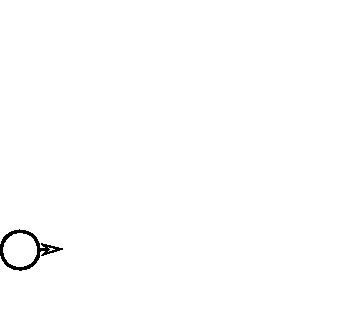
\includegraphics[width=0.44\textwidth]{slam_example_gt1.pdf}}
        }\hfill{}
        \subfloat[Sistema de SLAM del robot]
        {
            \fbox{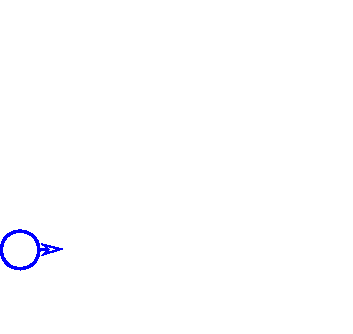
\includegraphics[width=0.44\textwidth]{slam_example_robot1.pdf}}
        }
    \end{figure}
    
\end{frame}

\begin{frame}
    \frametitle{Ejemplo de SLAM}
    
    \begin{figure}
        \subfloat[Realidad]
        {
            \fbox{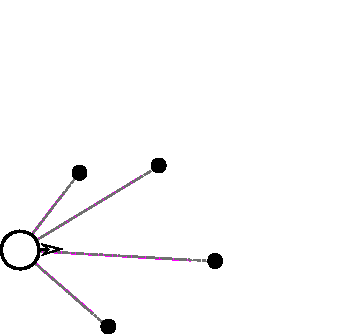
\includegraphics[width=0.44\textwidth]{slam_example_gt2.pdf}}
        }\hfill{}
        \subfloat[Sistema de SLAM del robot]
        {
            \fbox{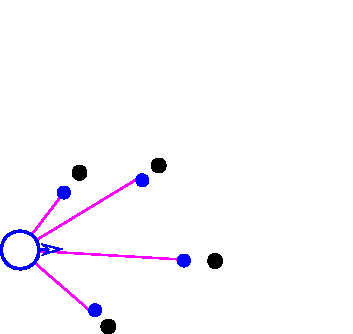
\includegraphics[width=0.44\textwidth]{slam_example_robot2.pdf}}
        }
    \end{figure}
    
\end{frame}

\begin{frame}
    \frametitle{Ejemplo de SLAM}
    
    \begin{figure}
        \subfloat[Realidad]
        {
            \fbox{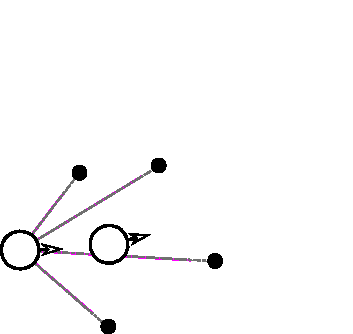
\includegraphics[width=0.44\textwidth]{slam_example_gt3.pdf}}
        }\hfill{}
        \subfloat[Sistema de SLAM del robot]
        {
            \fbox{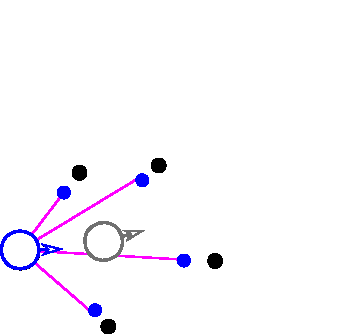
\includegraphics[width=0.44\textwidth]{slam_example_robot3.pdf}}
        }
    \end{figure}
    
\end{frame}

\begin{frame}
    \frametitle{Ejemplo de SLAM}
    
    \begin{figure}
        \subfloat[Realidad]
        {
            \fbox{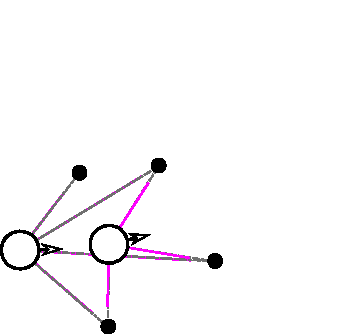
\includegraphics[width=0.44\textwidth]{slam_example_gt4.pdf}}
        }\hfill{}
        \subfloat[Sistema de SLAM del robot]
        {
            \fbox{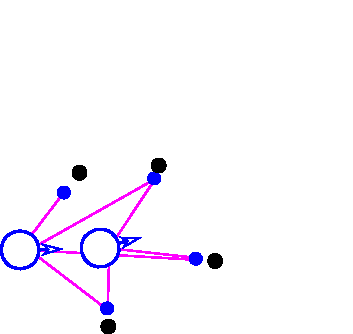
\includegraphics[width=0.44\textwidth]{slam_example_robot4.pdf}}
        }
    \end{figure}
    
\end{frame}

\begin{frame}
    \frametitle{Ejemplo de SLAM}
    
    \begin{figure}
        \subfloat[Realidad]
        {
            \fbox{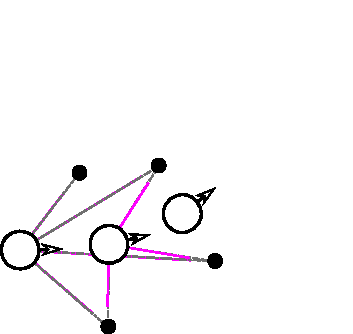
\includegraphics[width=0.44\textwidth]{slam_example_gt5.pdf}}
        }\hfill{}
        \subfloat[Sistema de SLAM del robot]
        {
            \fbox{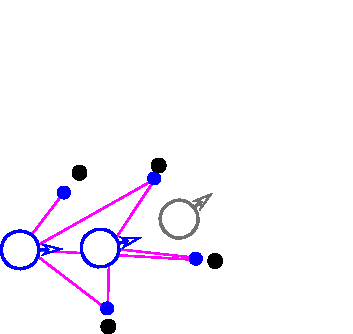
\includegraphics[width=0.44\textwidth]{slam_example_robot5.pdf}}
        }
    \end{figure}
    
\end{frame}

\begin{frame}
    \frametitle{Ejemplo de SLAM}
    
    \begin{figure}
        \subfloat[Realidad]
        {
            \fbox{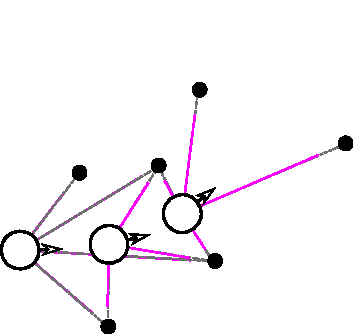
\includegraphics[width=0.44\textwidth]{slam_example_gt6.pdf}}
        }\hfill{}
        \subfloat[Sistema de SLAM del robot]
        {
            \fbox{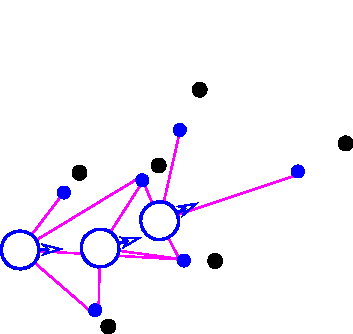
\includegraphics[width=0.44\textwidth]{slam_example_robot6.pdf}}
        }
    \end{figure}
    
\end{frame}

\begin{frame}
    \frametitle{Ejemplo de SLAM}
    
    \begin{figure}
        \subfloat[Realidad]
        {
            \fbox{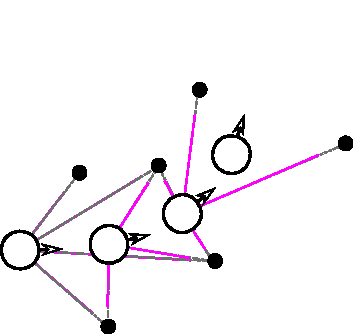
\includegraphics[width=0.44\textwidth]{slam_example_gt7.pdf}}
        }\hfill{}
        \subfloat[Sistema de SLAM del robot]
        {
            \fbox{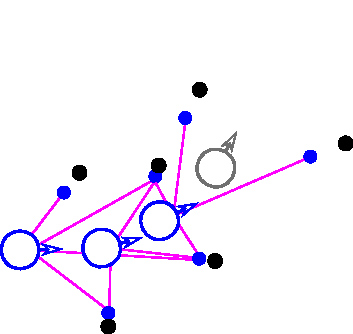
\includegraphics[width=0.44\textwidth]{slam_example_robot7.pdf}}
        }
    \end{figure}
    
\end{frame}

\begin{frame}
    \frametitle{Ejemplo de SLAM}
    
    \begin{figure}
        \subfloat[Realidad]
        {
            \fbox{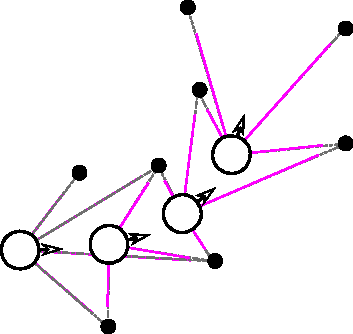
\includegraphics[width=0.44\textwidth]{slam_example_gt8.pdf}}
        }\hfill{}
        \subfloat[Sistema de SLAM del robot]
        {
            \fbox{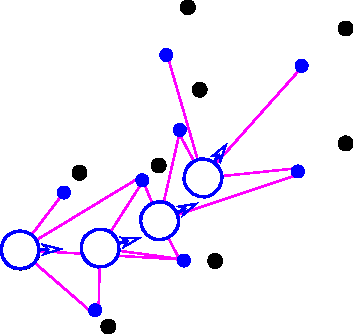
\includegraphics[width=0.44\textwidth]{slam_example_robot8.pdf}}
        }
    \end{figure}
    
\end{frame}

\begin{frame}
    \frametitle{Aquitectura general de SLAM}
    
    \begin{figure}[!h]
            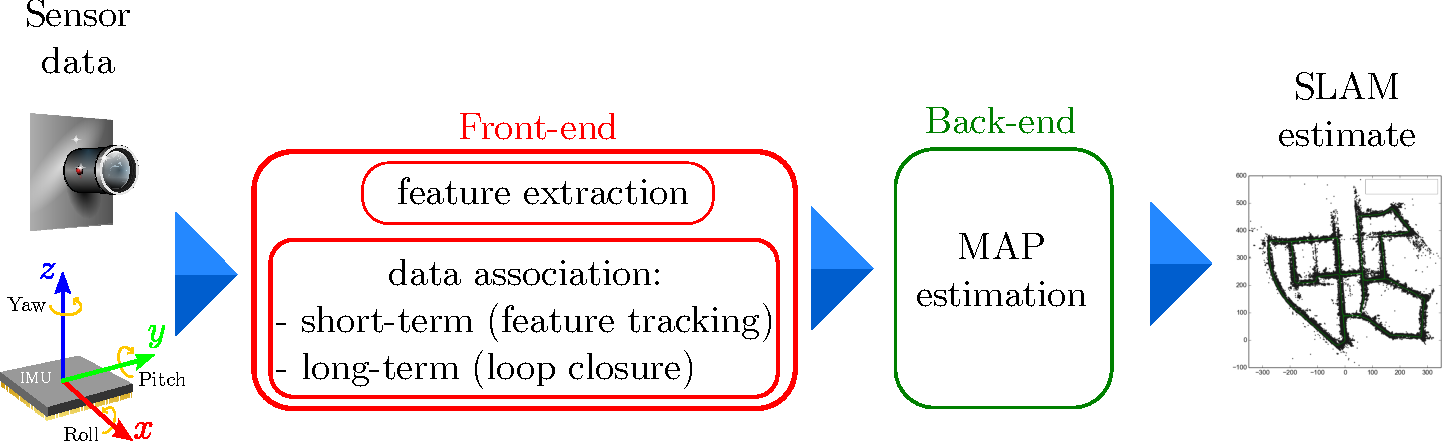
\includegraphics[width=\textwidth]{images/slam_frontend_backend.pdf}
    \end{figure}
    
\end{frame}

\begin{frame}
    \frametitle{Tipos de SLAM Back-ends}
    \note{Información extraída de https://youtu.be/BuRCJ2fegcc y de https://youtu.be/Alu59K8zvYs}
    \footnotesize
    \begin{itemize}
        \item Basados en Kalman Filter (EKF-SLAM)
        \item Basados en Particle Filter (FastSLAM, Rao-Blackwellized Particle Filter, Gmapping)
        \item Basados en Least-Squares (Graph-SLAM, Bundle Adjustment)
        \begin{itemize}
            \item Pose-Graph (solo contiene las poses del robot, el mapa es marginalizado\footnote{Marginalizar es el proceso de remover variables sin perder información.})
            \item Factor-Graph (contiene poses y landmarks)
        \end{itemize}
            Herramientas de optimización
            \begin{itemize}
            \item Ceres
            \item GTSAM
            \item g2o
            \end{itemize}
    \end{itemize}

    \begin{center}
        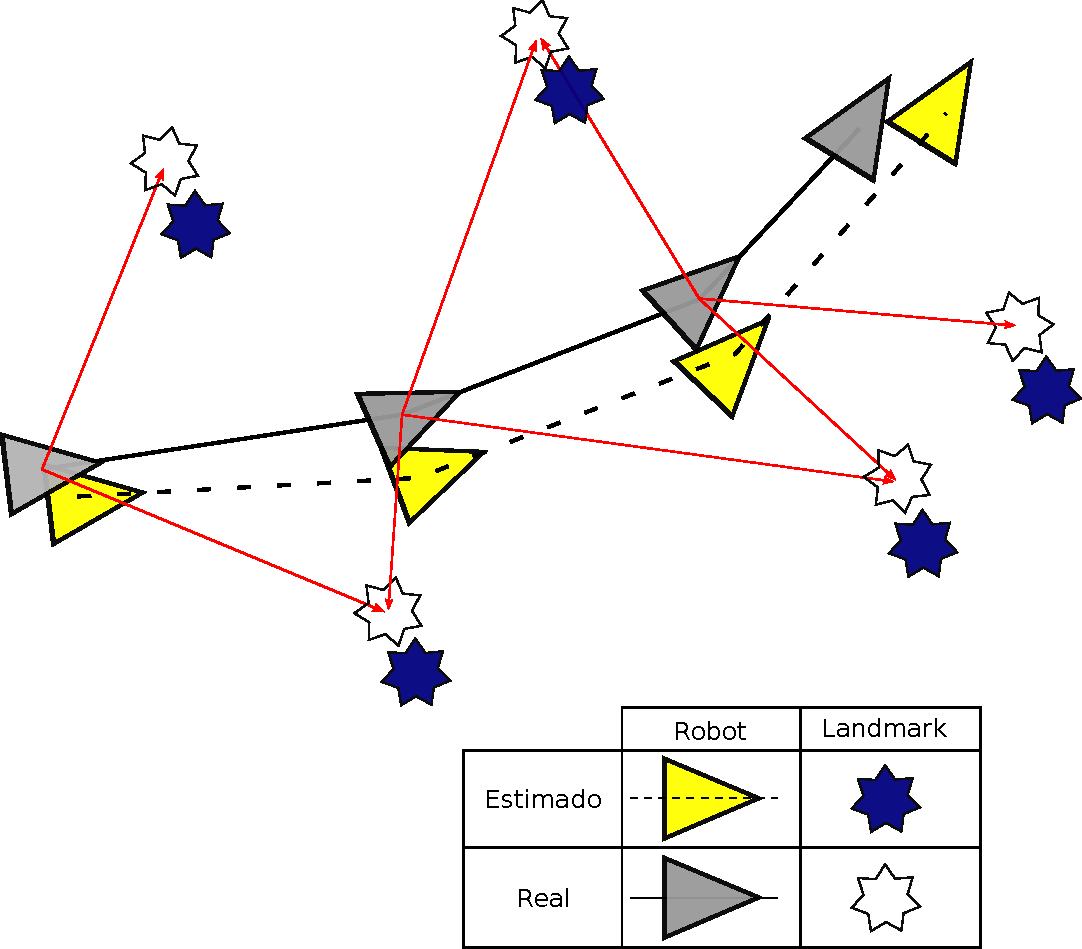
\includegraphics[width=0.25\textwidth]{images/slam-landmarks.pdf}
    \end{center}
    
\end{frame}

\begin{frame}
    \frametitle{Graph-SLAM}
    
    Graph-SLAM: construir un grafo y encontrar una configuración de nodos que minimiza el error introducido por las restricciones (aristas)
    
    \begin{itemize}
        \item Se utiliza un grafo para representar el problema.
        \item Los nodos representan poses o ubicaciones de landmarks.
        \item Las aristas son observaciones de landmarks o mediciones de odometría
        \item La minimización optimiza las poses del robot y la ubicación del los landmarks
        \item Observar áreas previamente vistas genera restricciones en el grafo
    \end{itemize}

    \begin{figure}
    \subfloat[]
    {
        \fbox{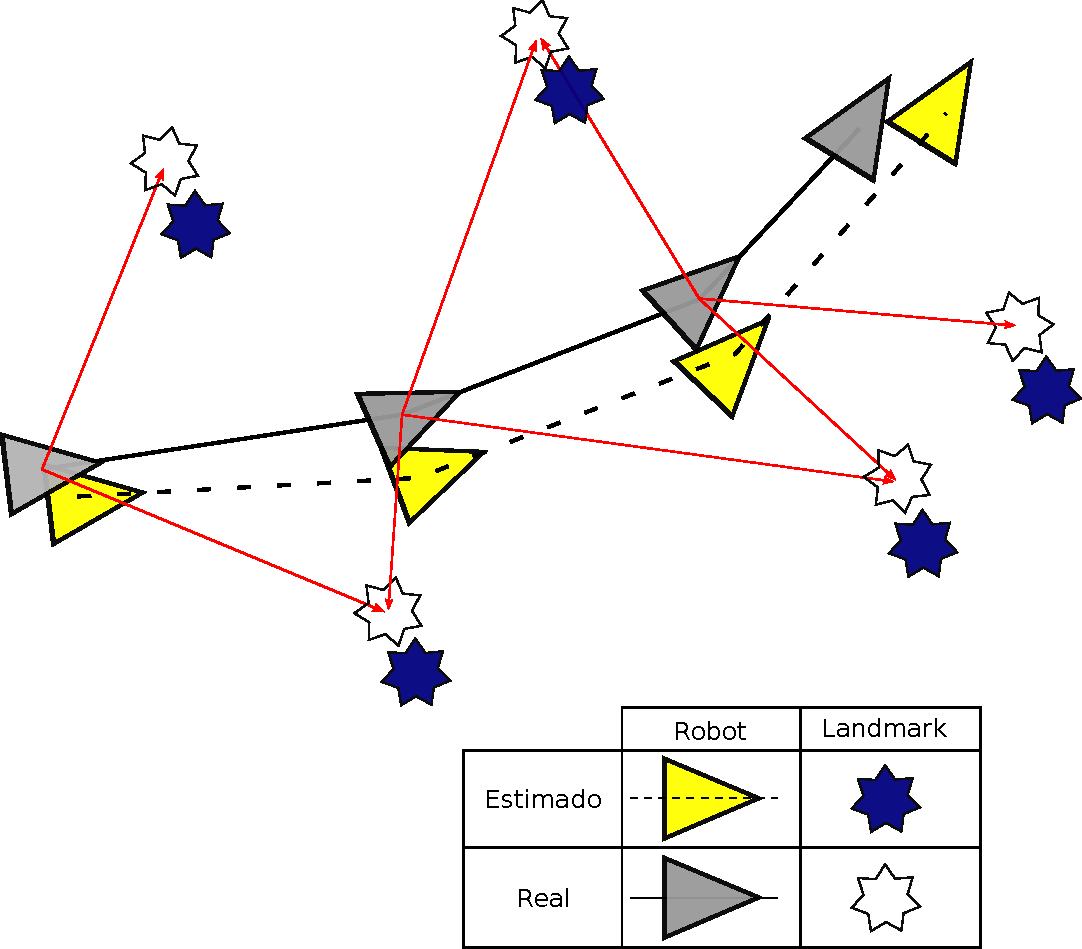
\includegraphics[width=0.25\textwidth]{images/slam-landmarks.pdf}}
    }\hspace{1em}
    \subfloat[]
    {
        \fbox{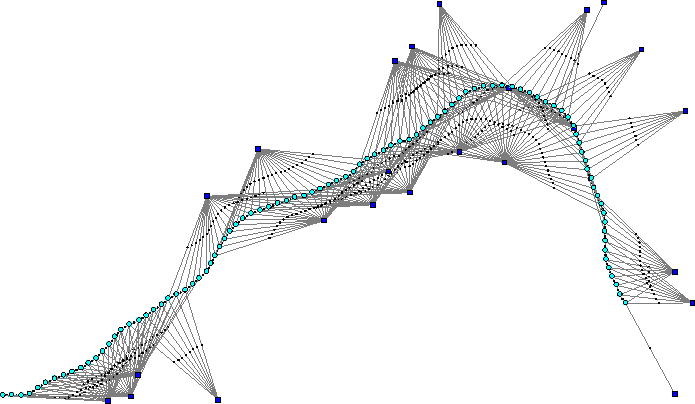
\includegraphics[width=0.375\textwidth]{images/factor_graph.pdf}}
    }
    \end{figure}
    
\end{frame}


\begin{frame}
    \frametitle{Factor-Graph}
    \note{Información extraída de https://youtu.be/uuiaqGLFYa4}
    
    \begin{block}{Factor-Graph}
        Un Factor-graph es un término matemático, un grafo bipartito representando la factorización de una función. Esto significa que podemos tomar una función por ejemplo $g(.)$ y descomponerla mediante el producto de funciones $f(.)$,
        
        \begin{equation*}
            g(X_{1}, \dots, X_{n}) = \prod_{i} f_{i}(S_{i}) \quad \text{con} \quad S_{i}     \subseteq \{ X_{1},\dots, X_{n} \}
        \end{equation*}
    \end{block}

    \begin{figure}[!h]
        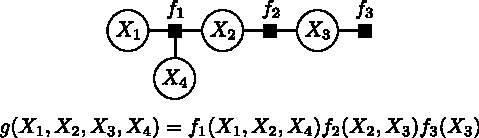
\includegraphics[width=0.7\textwidth]{images/factor_graph_example.pdf}
    \end{figure}

    \note{Por ejemplo, si la función g depende de 10 variables podemos descomponerla en el profucto de varias funciones f, donde cada función f depende de un subconjunto de esas variables.}
    
\end{frame}


\begin{frame}
    \frametitle{Factor-Graph}
    \note{Información extraída de https://youtu.be/uuiaqGLFYa4}
    
    \begin{itemize}
        \item Los Factor-Graph nos permiten representar una distribución de probabilidad conjunta (distribución que gobierna sobre todas las variables) como un producto de probabilidades más chicas (que dependen de un menor número de variables).
        \item Al igual que las redes de Bayes o redes de Markov, podemos utilizar los Factor-Graph para describir cómo las variables dependen entre si. Y podemos correr diferentes algoritmos sobre estos Factor-Graph para inferir información de una manera eficiente.
        \item Ejemplo de algorimo que trabaja sobre Factor-graph, es el Algoritmo de Sum-product para el computo de distribuciones marginales (distribuciones que solamente dependen un subconjunto de variables).
        \item En el contexto de robótica los Factor-graph son utilizados para especificar problemas de mínimos cuadrados. El factor graph nos permite representar cómo ciertos estados dependen o estan relacionados entre sí basados en la información que tenemos de las mediciones de los sensores (almacenada en los factores).
    \end{itemize}
    
    \note{Por ejemplo, si la función g depende de 10 variables podemos descomponerla en el profucto de varias funciones f, donde cada función f depende de un subconjunto de esas variables.}
    
\end{frame}

\begin{frame}
    \frametitle{Graph-based SLAM usando Pose-Graph}
    \note{Información extraída de https://youtu.be/uHbRKvD8TWg}
    
    \begin{itemize}
        \item Las restricciones conectan las poses del robot mientras se desplaza
        \item Las restricciones tiene ruido
    \end{itemize}

    \begin{figure}[!h]
        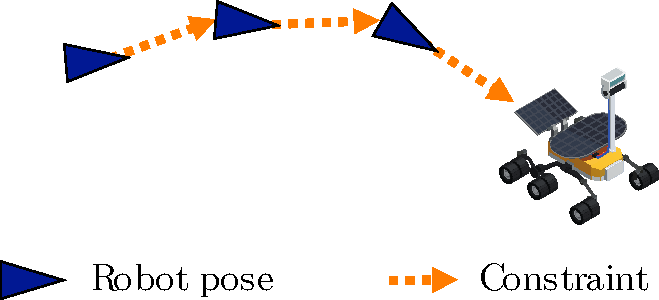
\includegraphics[width=0.7\textwidth]{images/pose_graph_example.pdf}
    \end{figure}
    
\end{frame}

\begin{frame}
    \frametitle{Graph-based SLAM usando Pose-Graph}
    \note{Información extraída de https://youtu.be/uHbRKvD8TWg}
    
    \begin{itemize}
        \item Observando áreas previamente vistas se generan restricciones entre poses no consecutivas (\emph{Loop Closure})
    \end{itemize}
    
       \begin{figure}[!h]
        \includegraphics[width=0.4\textwidth]{images/pose_graph_loop_example.pdf}
    \end{figure}
    
\end{frame}

\begin{frame}[fragile]
    \frametitle{2D Pose-Graph con LiDAR}
    \note{Víðeo extraído de https://youtu.be/E6IvbjZA7Ao}
        
    \begin{center}
    \movie[loop]{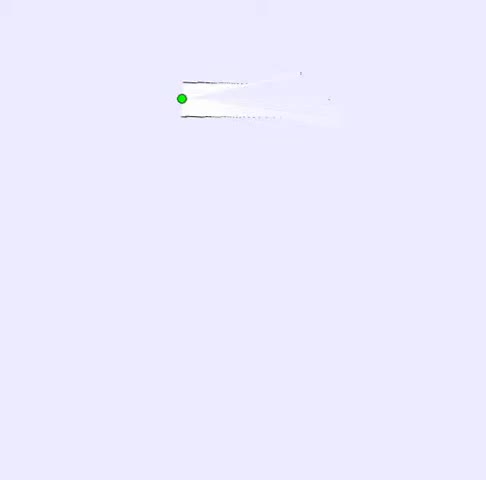
\includegraphics[width=0.5\columnwidth]{./images/pose_graph_2d_video.jpg}}{./videos/pose_graph_2d.mp4}
    \end{center}
    
\end{frame}


\begin{frame}
    \frametitle{Graph-based SLAM usando Pose-Graph}
    \note{Información extraída de https://youtu.be/uHbRKvD8TWg}
    
    \begin{columns}
        \begin{column}{0.5\textwidth}
        \begin{itemize}
            \item<1-2> Cada nodo es una pose del robot junto con su medición de laser (no hay landmarks)
            \item<1-2> Cada arista corresponde a una restricción espacial entre los nodos que relaciona.
            \item<3-> Una vez que tenemos el grafo, obtenemos el mapa mas probable mediante la corrección de los nodos
            \item<4-> así...
            \item<5> Dibujamos el mapa basandonos en las poses corregidas
        \end{itemize}
        \end{column}
        \begin{column}{0.5\textwidth}  %%<--- here
                \only<1>{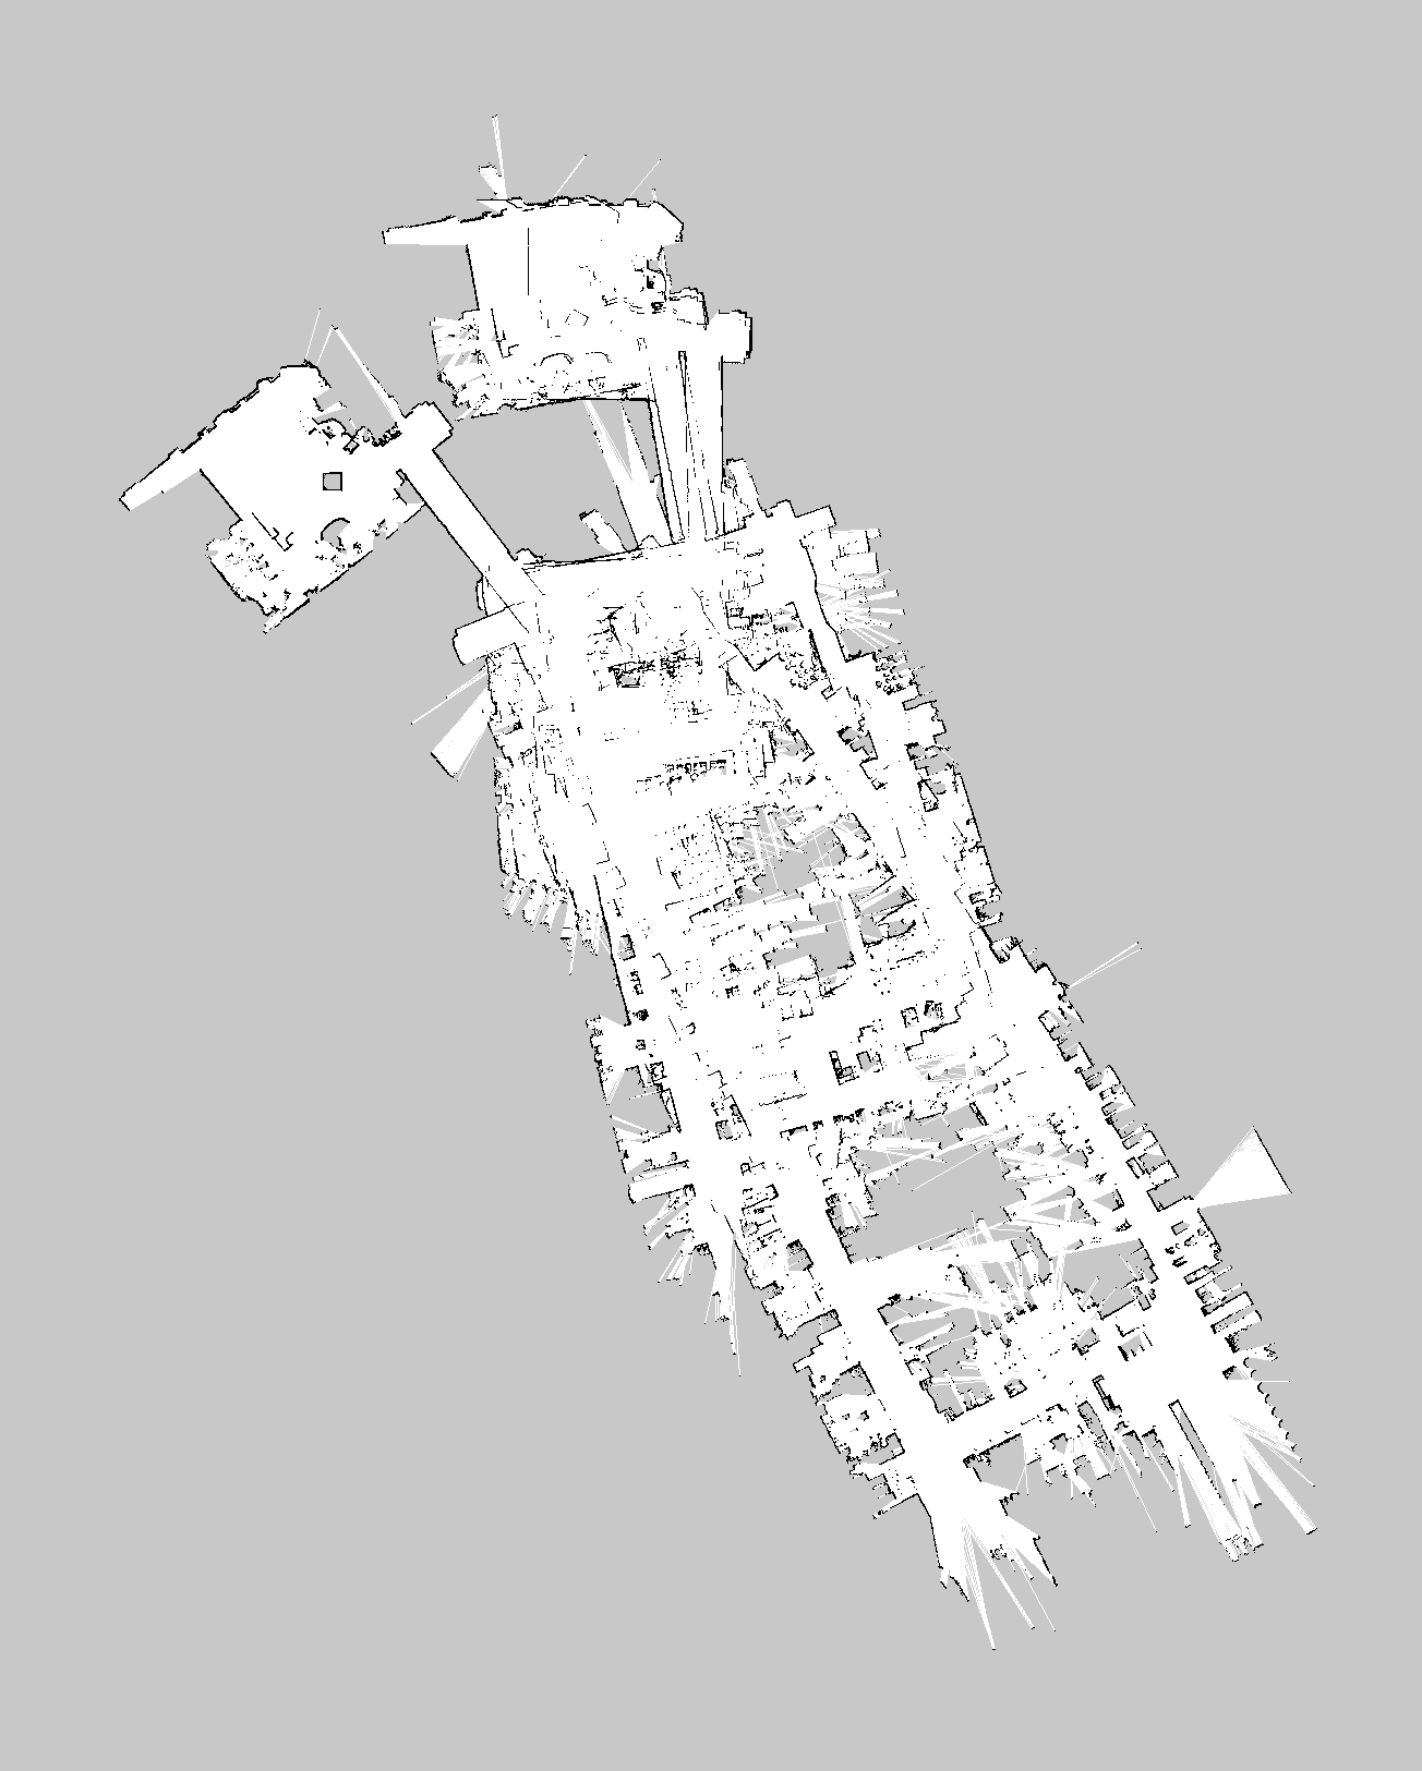
\includegraphics[width=0.7\textwidth]{images/pose_graph_map.png}}
                \only<2>{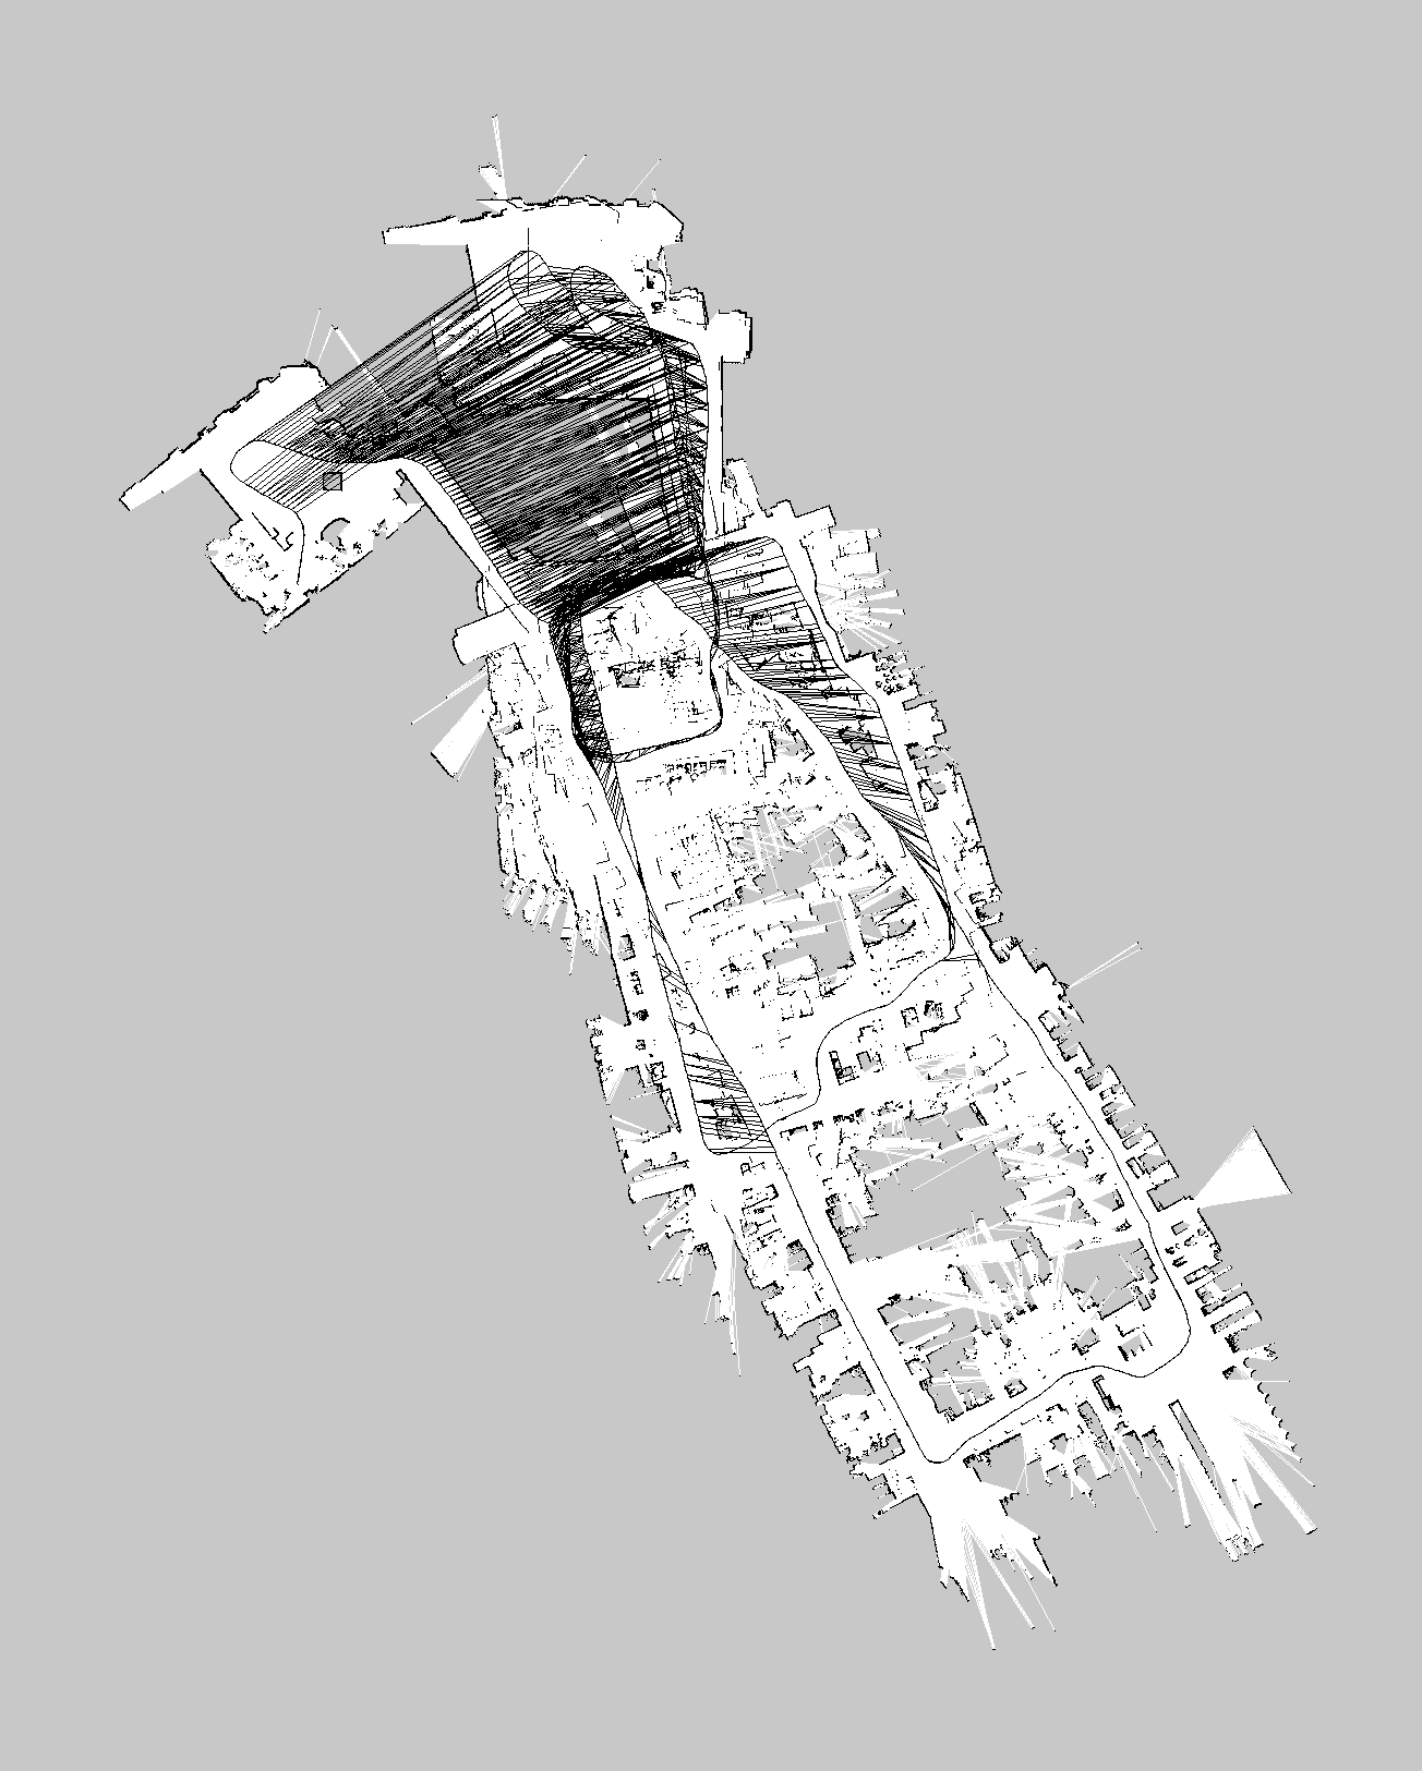
\includegraphics[width=0.7\textwidth]{images/pose_graph_constraints_with_map.png}}
                \only<3>{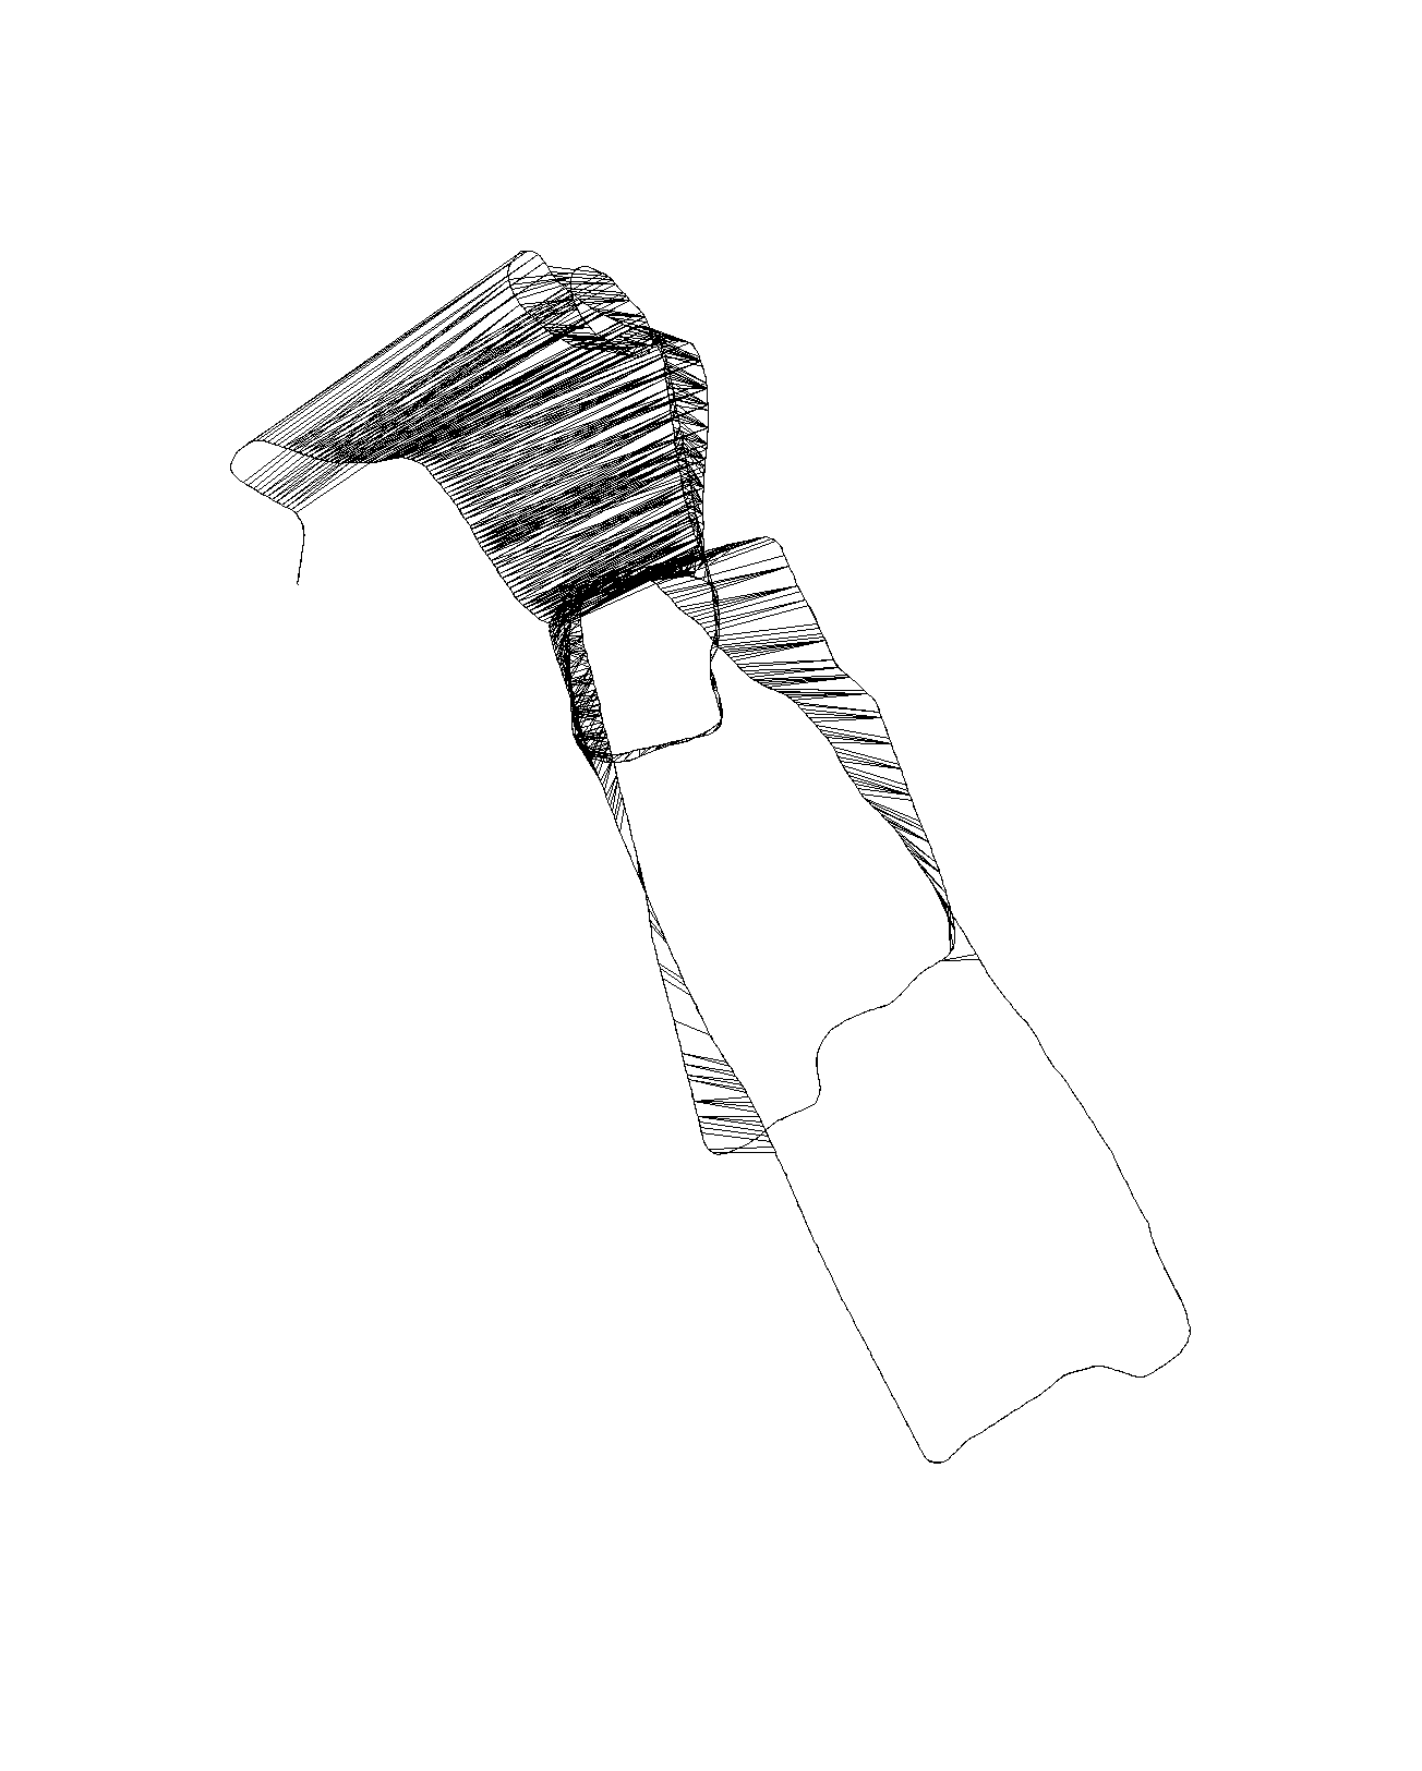
\includegraphics[width=0.7\textwidth]{images/pose_graph_constraints.png}}
                \only<4>{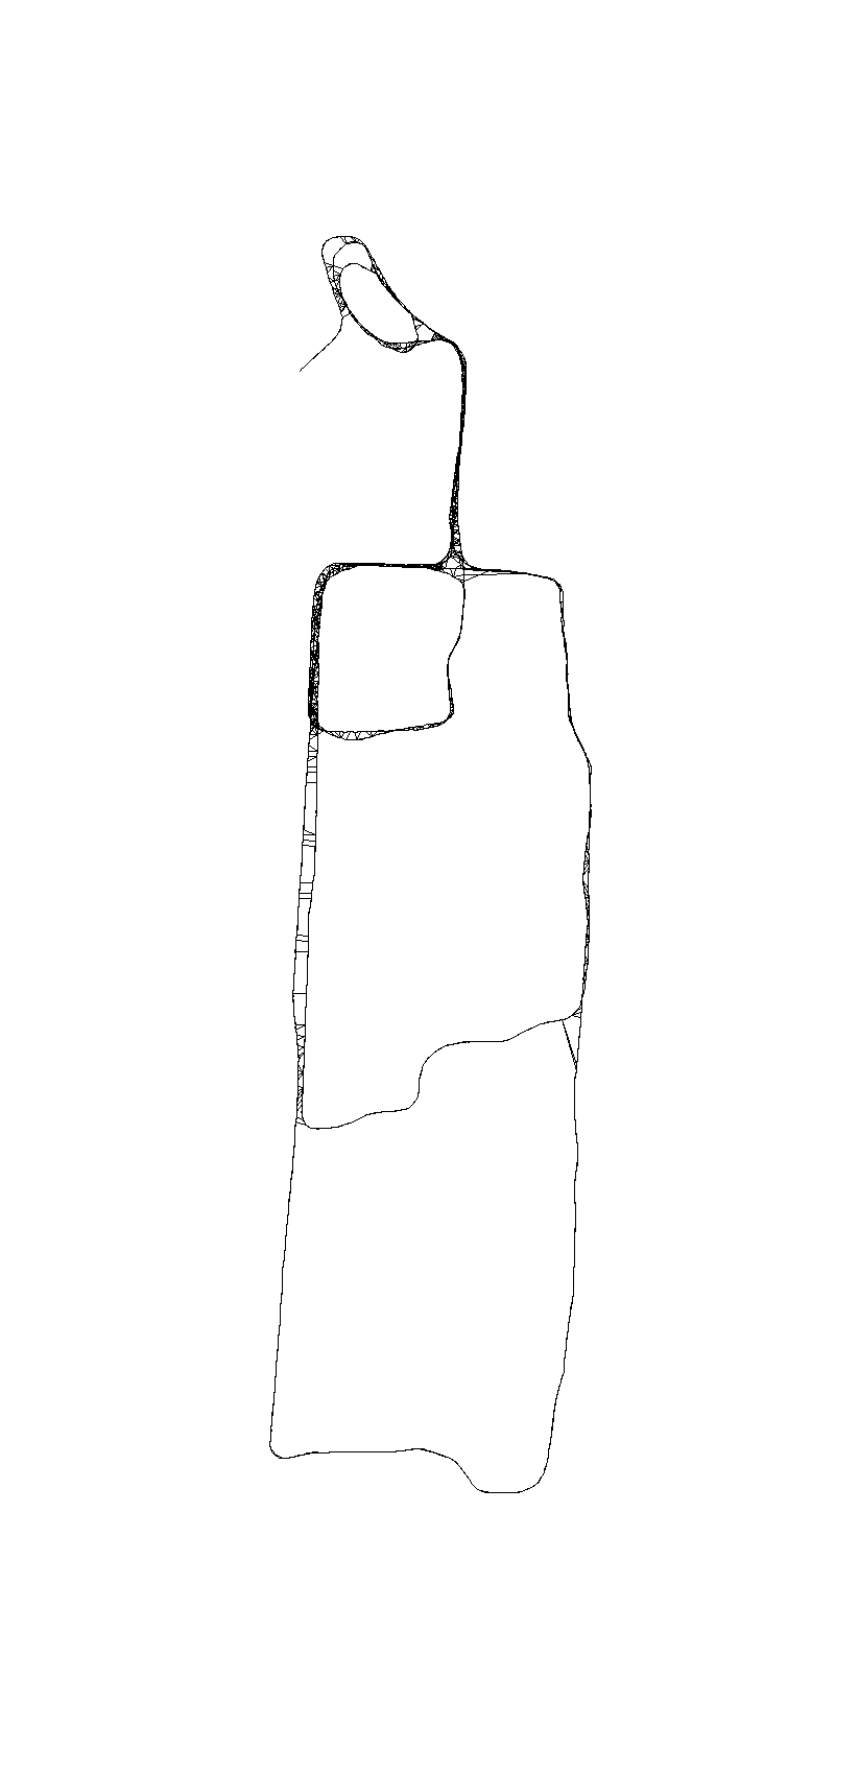
\includegraphics[width=0.5\textwidth]{images/pose_graph_optimized.png}}
                \only<5>{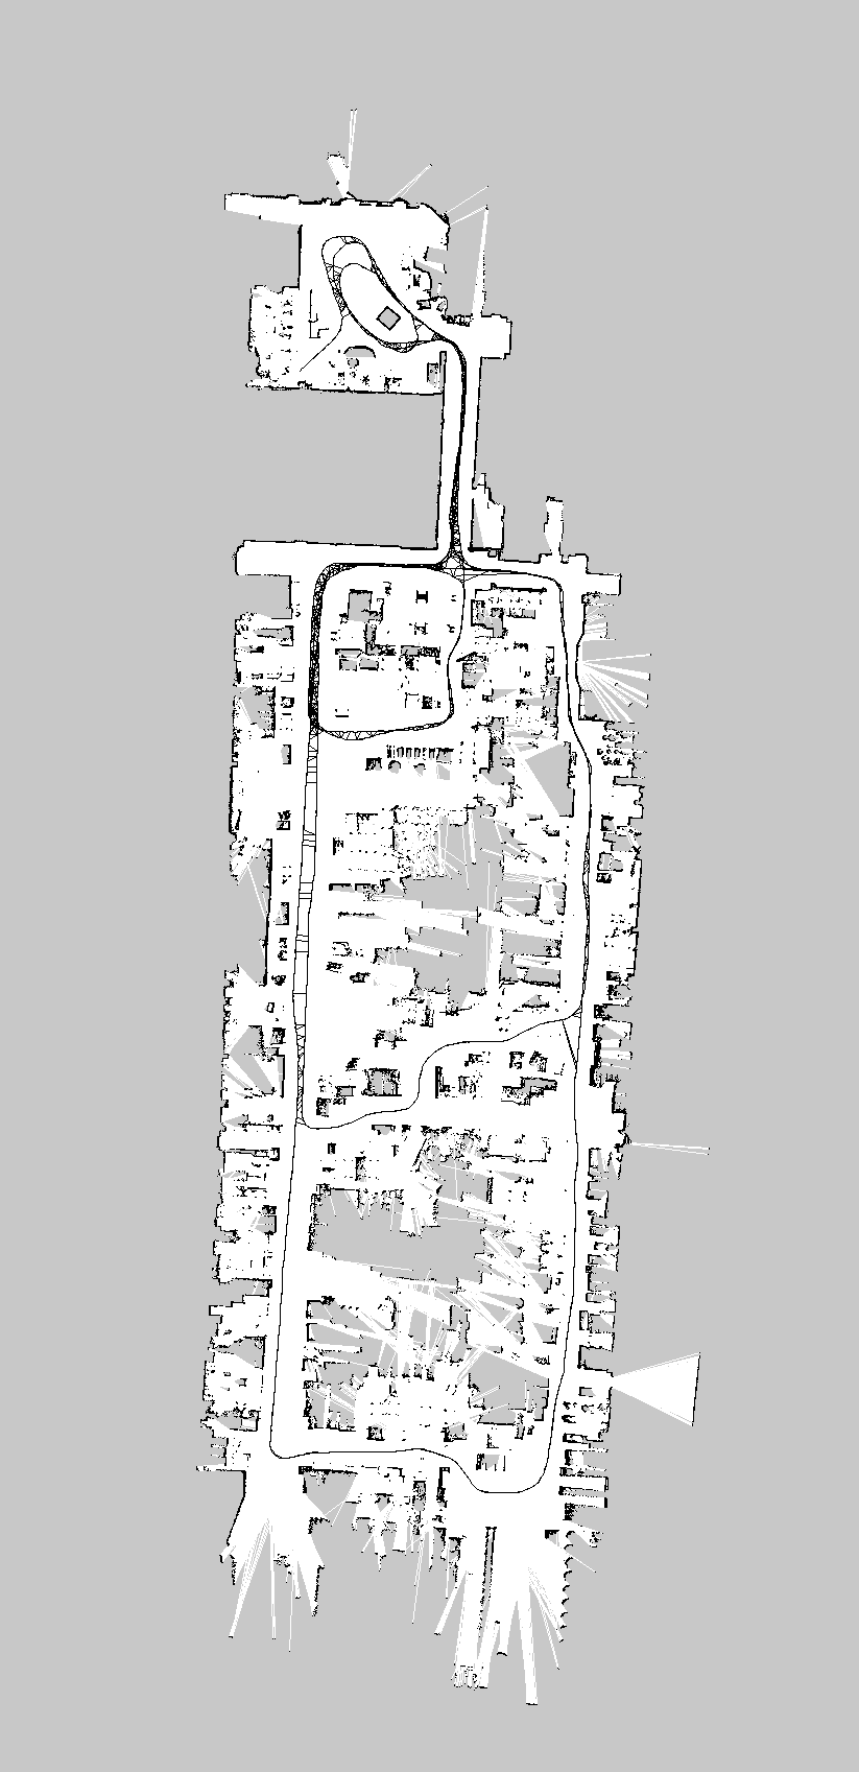
\includegraphics[width=0.5\textwidth]{images/pose_graph_optimized_with_map.png}}
        \end{column}
    \end{columns}
    
\end{frame}

\begin{frame}
    \frametitle{El grafo en pose-graph}
    \note{Información extraída de https://youtu.be/uHbRKvD8TWg}
    
    \begin{itemize}
        \item Consiste en $n$ nodos $\stateBold = \stateBold_{1:n}$
        \item Cada $\stateBold_{i}$ es una pose del robot en el tiempo $t_{i}$
        \item Una restricción/arista existe entre el nodo $\stateBold_{i}$ y $\stateBold_{j}$ si ...
    \end{itemize}
    
     \begin{figure}[!h]
        \includegraphics[width=0.3\textwidth]{pose_graph_loop_example.pdf}
    \end{figure}
    
\end{frame}

\begin{frame}
    \frametitle{Crear una arista si...}
    \note{Información extraída de https://youtu.be/uHbRKvD8TWg}
    
    \begin{itemize}
        \item Una restricción/arista existe entre el nodo $\stateBold_{i}$ y $\stateBold_{j}$ si el robot se mueve de $\stateBold_{i}$ a $\stateBold_{i+1}$
        \item Las aristas corresponden a odometría
    \end{itemize}
    
    \begin{figure}[!h]
        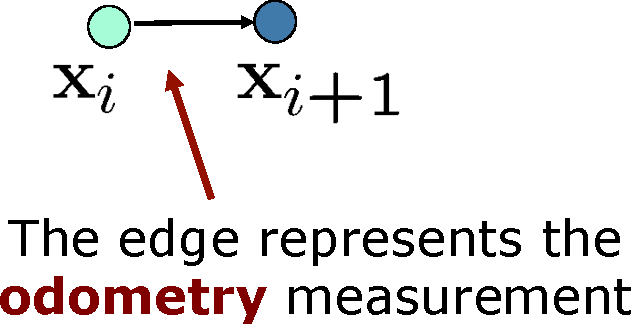
\includegraphics[width=0.44\textwidth]{pose_graph_odometry_edge.pdf}
    \end{figure}
    
\end{frame}


\begin{frame}
    \frametitle{Crear una arista si...}
    \note{Información extraída de https://youtu.be/uHbRKvD8TWg}
    
    \begin{itemize}
        \item<1-> Una restricción/arista existe entre el nodo $\stateBold_{i}$ y $\stateBold_{j}$ si el robot observa la misma parte del entorno desde $\stateBold_{i}$ y desde $\stateBold_{j}$
        \item<2>  Construimos una {\bf restricción virtual} entre la posición de $\stateBold_{j}$ vista desde $\stateBold_{i}$
    \end{itemize}
    \only<1>{
        \begin{figure}
            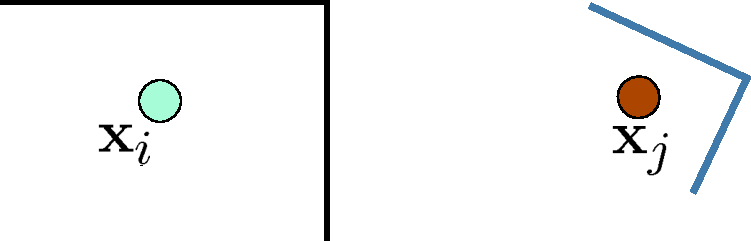
\includegraphics[width=0.44\textwidth]{pose_graph_edge_lidar.pdf}
        \end{figure}
    }
    \only<2>{
        \begin{figure}
            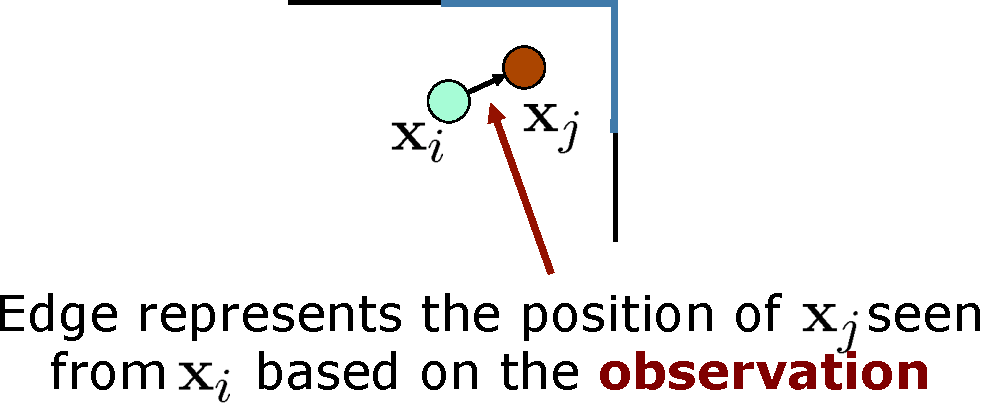
\includegraphics[width=0.44\textwidth]{pose_graph_edge_lidar2.pdf}
        \end{figure}
    }
    
\end{frame}

\begin{frame}
    \frametitle{La matriz de información de las aristas}
    \note{Información extraída de https://youtu.be/uHbRKvD8TWg}
    \begin{itemize}
        \item Las observaciones tienen ruido
        \item La matriz de información $\informationMatrix_{ij}$ para cada arista codifica su incertidumbre
        \item Mientras más grande $\informationMatrix_{ij}$, más importa la arista en al optimización.
    \end{itemize}
    
\end{frame}

\begin{frame}
    \frametitle{La matriz de información de las aristas}
    \note{Información extraída de https://youtu.be/uHbRKvD8TWg}
    \begin{figure}[!h]
        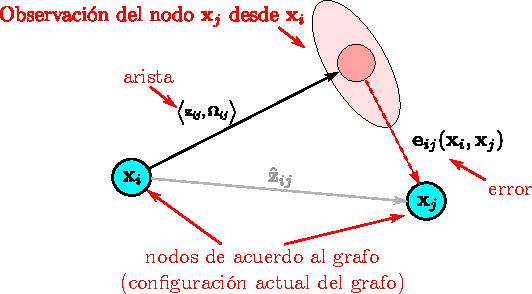
\includegraphics[width=0.7\textwidth]{images/factor_graph_edge_example.pdf}
    \end{figure}

    Objetivo:
    \begin{equation*}
        \stateBold^{*} = \argmin_{\stateBold} \sum_{ij} \error^{\top}_{ij} \informationMatrix_{ij} \error_{ij}
    \end{equation*}
    
\end{frame}



\begin{frame}
    \frametitle{Mínimos cuadrados en SLAM}
    \note{Información extraída de https://youtu.be/uHbRKvD8TWg}
    Podemos minimizar el error utilizaremos mínimos cuadrados (\emph{Least Square})
    \begin{align*}
        \state^{*} &= \argmin_{\stateBold} \sum_{ij} \error^{\top}_{ij}(\stateBold_{i},\stateBold_{j}) \informationMatrix_{ij} \error_{ij}(\stateBold_{i},\stateBold_{j})\\
                 &= \argmin_{\stateBold} \sum_{k} \error^{\top}_{k}(\stateBold) \informationMatrix_{k} \error_{k}(\stateBold)
    \end{align*}
    
    El {\bf vector estado} es la concatenación de los nodos pose $\stateBold = (\stateBold_{1}^{\top} \stateBold_{2}^{\top} \dots \stateBold_{n}^{\top})$. Cada nodo es una pose (posición u orientación).
    
    \vspace{2em}
    {\bf Tenemos que definir la función de error...}
\end{frame}


\begin{frame}
    \frametitle{Función de error}
    \note{Información extraída de https://youtu.be/uHbRKvD8TWg}
    
    \begin{itemize}
    \item Función de error para una sola restricción
           \begin{figure}
            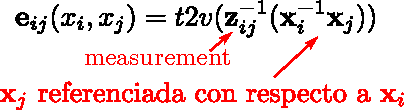
\includegraphics[width=0.44\textwidth]{pose_graph_error_function.pdf}
        \end{figure}
    \footnotetext{$t2v(.)$ mapea transformaciones a vectores}
    
    \item Error como una función de un vector estado completo
    
    \begin{equation*}
        \error_{ij}(\state) = t2v(\inverse{\observationBold}_{ij}(\inverse{\stateBold}_{i}\stateBold_{j}))
    \end{equation*}

    \item El error toma el valor 0 cuando
    
    \begin{equation*}
        \observationBold_{ij} = (\inverse{\stateBold}_{i}\stateBold_{j})
    \end{equation*}
    
    \end{itemize}
\end{frame}

\begin{frame}
    \frametitle{Método de Gauss-Newton para la minimización del error}
    \note{Información extraída de https://youtu.be/uHbRKvD8TWg}
    
    \begin{itemize}
        \item Definir la función de error
        \item Linearizar la función de error
        \item Calcular las derivadas
        \item Igualar las derivadas a cero
        \item Resolver el sistema lineal
        \item Iterar este procedimiento hasta que converja
    \end{itemize}

\end{frame}


\begin{frame}
    \frametitle{Ejemplo de Mimimización con Gauss-Newton}
    \note{Información extraída de https://youtu.be/r2cyMQ5NB1o?si=lRbB_CJmqnsFsktT}
    
    %\TODO{Ver \url{https://youtu.be/CJE59i8oxIE?si=3RmiP3UM2ImEj-av} para ejemplo de aplicación de Gauss-Newton}
   
    
   
\end{frame}


\begin{frame}
    \frametitle{Linearizar la función de error}
    \note{Información extraída de https://youtu.be/uHbRKvD8TWg}
    
    \begin{itemize}
        \item Podemos aproximar el error al rededor de una estimación inicial $\state$ a través de una expansión de Taylor
    \end{itemize}

    \begin{equation*}
        \error_{ij}(\stateBold + \vec{\Delta}\stateBold) \simeq  \error_{ij}(\stateBold) + \jacobian_{ij}\vec{\Delta}\stateBold \quad \text{con} \quad \jacobian_{ij} = \dfrac{\partial\error_{ij}(\stateBold)}{\partial\stateBold}
    \end{equation*}
    
\end{frame}

\begin{frame}
    \frametitle{Derivada de la función de error}
    \note{Información extraída de https://youtu.be/uHbRKvD8TWg}
    \begin{itemize}
        \item<1-> Pregunta: ¿Depende un término de error $\error_{ij}(\stateBold)$ de todas las variables de estado?
        
        \only<2->{No, solo depende de $\stateBold_{i}$ y $\stateBold_{j}$}
        
        \item<3-> Pregunta: ¿Hay alguna consecuencia en la estructura del Jacobiano?
        
        \only<4->{
            Si, será diferente a cero solamente en las filas correspondientes a  $\stateBold_{i}$ y $\stateBold_{j}$
        
            \begin{align*}
                \dfrac{\partial\error_{ij}(\stateBold)}{\partial\stateBold} &= 
                \begin{bmatrix}
                    0 & \dots & \dfrac{\partial\error_{ij}(\stateBold_{i})}{\partial\stateBold_{i}} & \dots & 0 & \dots & \dfrac{\partial\error_{ij}(\stateBold_{j})}{\partial\stateBold_{j}} & \dots & 0
                \end{bmatrix} \\
                \jacobian_{ij} &= 
                    \begin{bmatrix}
                        0 & \dots & \vec{A}_{ij} & \dots & 0 & \dots & \vec{B}_{ij} & \dots & 0
                    \end{bmatrix}
            \end{align*}
        }
        
        
    \end{itemize}
    
\end{frame}


\begin{frame}
    \frametitle{Jacobianos y problema disperso}
    \note{Información extraída de https://youtu.be/uHbRKvD8TWg}
    
    \begin{itemize}
        \item El error $\error_{ij}(\stateBold)$ depende solamente de los bloques de parámetros $\stateBold_{i}$ y $\stateBold_{j}$
        
        \begin{equation*}
            \error_{ij}(\stateBold) =\error_{ij}(\stateBold_{i} ,\stateBold_{j})
        \end{equation*}
    
        \item El Jacobiano será cero en todos lados excepto en las columnas $\stateBold_{i}$ y $\stateBold_{j}$
        
           \begin{equation*}
            \jacobian_{ij} = 
            \begin{bmatrix}
                0 & \dots & 0 & \dfrac{\partial\error_{ij}(\stateBold_{i})}{\partial\stateBold_{i}} & 0 & \dots & 0 & \dfrac{\partial\error_{ij}(\stateBold_{j})}{\partial\stateBold_{j}} & 0 & \dots & 0
            \end{bmatrix}
        \end{equation*}
        
    \end{itemize}

    {\bf Esto nos permite resolver SLAM de manera eficiente!}
    
\end{frame}


\begin{frame}
    \frametitle{Consecuencia de que sea un problema disperso}
    \note{Información extraída de https://youtu.be/uHbRKvD8TWg}
    
    \begin{itemize}
        \item Necesitamos computar el vector coeficiente
        \begin{align*}
            \linearSystemb^{\top} &= \sum_{ij} \linearSystemb_{ij}^{\top} = \sum_{ij} \error_{ij}^{\top}\Omega_{ij}\jacobian_{ij}\\
            \linearSystemH &= \sum_{ij} \linearSystemH_{ij} = \sum_{ij} \jacobian_{ij}^{\top}\Omega_{ij}\jacobian_{ij}
        \end{align*}
        \item La estructura dispersa de $\jacobian_{ij}$ resultará en una estructura dispersa de $\linearSystemH$
        \item Esta estructura refleja la matriz de adyacencia del grafo
    \end{itemize}
    
\end{frame}

\begin{frame}
    \frametitle{Ilustración de la estructura}
    \note{Información extraída de https://youtu.be/uHbRKvD8TWg}
    
    \begin{figure}[!h]
        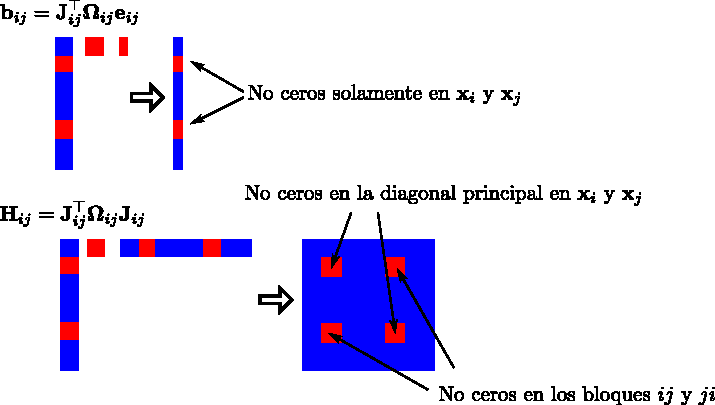
\includegraphics[width=0.9\textwidth]{linear_system_sparsity.pdf}
    \end{figure}
    
\end{frame}

\begin{frame}
    \frametitle{Consecuencia de que sea un problema disperso}
    \note{Información extraída de https://youtu.be/uHbRKvD8TWg}
    
     \begin{figure}[!h]
        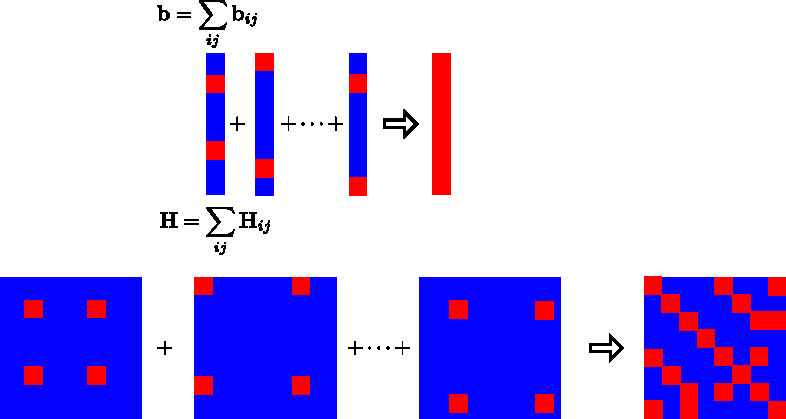
\includegraphics[width=0.9\textwidth]{linear_system_sparsity2.pdf}
    \end{figure}
    
\end{frame}

\begin{frame}
    \frametitle{Consecuencia de que sea un problema disperso}
    \note{Información extraída de https://youtu.be/uHbRKvD8TWg}
    
    \begin{itemize}
        \item Una arista contribuye al sistema lineal a través de $\linearSystemb_{ij}$ y $\linearSystemH_{ij}$
        \item El vector coeficiente es
        
        \begin{align*}
            \linearSystemb_{ij}^{\top} &= \error_{ij}^{\top}\informationMatrix_{ij}\jacobian_{ij}\\
            &= \error_{ij}^{\top}\informationMatrix_{ij}
                \begin{bmatrix}
                    0 & \dots & \vec{A}_{ij} & \dots & \vec{B}_{ij} & \dots & 0
                \end{bmatrix}\\
            &= 
                \begin{bmatrix}
                    0 & \dots & \error_{ij}^{\top}\informationMatrix_{ij}\vec{A}_{ij} & \dots & \error_{ij}^{\top}\informationMatrix_{ij}\vec{B}_{ij} & \dots & 0
                \end{bmatrix}
        \end{align*}
        \item Es diferente a cero solamente en los índices correspondientes de $\stateBold_{i}$ y $\stateBold_{j}$        
    \end{itemize}
    
\end{frame}

\begin{frame}
    \frametitle{Consecuencia de que sea un problema disperso}
    \note{Información extraída de https://youtu.be/uHbRKvD8TWg}
    
    \begin{itemize}
        \item La matriz coeficiente de una arista es

        \begin{align*}
            \linearSystemH_{ij}^{\top} &= \jacobian_{ij}^{\top}\informationMatrix_{ij}\jacobian_{ij}\\
            &= 
            \begin{bmatrix}
                \vdots \\
                \vec{A}_{ij}^{\top}\\
                \vdots \\
                \vec{B}_{ij}^{\top}\\
                \vdots
            \end{bmatrix} \informationMatrix_{ij}
            \begin{bmatrix}
                \cdots & \vec{A}_{ij} & \cdots & \vec{B}_{ij} & \cdots
            \end{bmatrix}\\
            &= 
            \begin{bmatrix}
                \vec{A}_{ij}^{\top}\informationMatrix_{ij}\vec{A}_{ij} & \vec{A}_{ij}^{\top}\informationMatrix_{ij}\vec{B}_{ij}\\
                \vec{B}_{ij}^{\top}\informationMatrix_{ij}\vec{A}_{ij} & \vec{B}_{ij}^{\top}\informationMatrix_{ij}\vec{B}_{ij}
            \end{bmatrix}
        \end{align*}
        \item Es diferente a cero en los bloques relacionados con $i,j$
    \end{itemize}
    
\end{frame}


\begin{frame}
    \frametitle{Resumen del problema disperso}
    \note{Información extraída de https://youtu.be/uHbRKvD8TWg}
    
    \begin{itemize}
        \item Una arista ij solo contribuye a
        \begin{itemize}
            \item i-ésimo y j-ésimo bloques de $\linearSystemb_{ij}$
            \item los bloques $ii$, $jj$, $ij$ y $ji$ de $\linearSystemH_{ij}$
        \end{itemize}
        \item El sistema resultante es disperso
        \item El sistema se puede computar sumando las contribuciones de cada arista
        \item Se pueden utilizar diferentes \emph{solvers}
        \begin{itemize}
            \item Descomposición de Sparse Cholesky
            \item Gradiente conjudado
            \item muchos más...
        \end{itemize}

    \end{itemize}
    
    
\end{frame}

\begin{frame}
    \frametitle{El sistema Lineal}
    \note{Información extraída de https://youtu.be/uHbRKvD8TWg}
    
    \begin{itemize}
        \item Vector de incrementos de estado
        \begin{equation*}
            \Delta\stateBold^{\top} =
            \begin{bmatrix}
            \Delta\stateBold_{1}^{\top}    & \Delta\stateBold_{2}^{\top} & \cdots & \Delta\stateBold_{n}^{\top}
            \end{bmatrix}
        \end{equation*}
    \item Vector coeficiente
        \begin{equation*}
            \linearSystemb^{\top} =
            \begin{bmatrix}
                \overline{\linearSystemb}_{1}^{\top} & \overline{\linearSystemb}_{2}^{\top} & \cdots & \overline{\linearSystemb}_{n}^{\top}
            \end{bmatrix}
        \end{equation*}
    \item Matriz de ecuaciones normales
        \begin{equation*}
            \linearSystemH =
            \begin{bmatrix}
            \overline{\linearSystemH}_{11} & \overline{\linearSystemH}_{12} & \cdots & \overline{\linearSystemH}_{1n}\\
            \overline{\linearSystemH}_{21} & \overline{\linearSystemH}_{22} & \cdots & \overline{\linearSystemH}_{2n}\\
            \vdots & \vdots & \ddots & \vdots\\
            \overline{\linearSystemH}_{n1} & \overline{\linearSystemH}_{n2} & \cdots & \overline{\linearSystemH}_{nn}\\
            \end{bmatrix}
        \end{equation*}
    \end{itemize}

\end{frame}

\begin{frame}
    \frametitle{Construcción del sistema lineal}
    \note{Información extraída de https://youtu.be/uHbRKvD8TWg}
    Para cada restricción:
    \begin{itemize}
        \item Computar el error $\error_{ij} = t2v(\inverse{\observationBold}_{ij}(\inverse{\stateBold}_{i}\stateBold_{j}))$
        \item Computar los bloques de los jacobianos:
            \begin{equation*}
                \vec{A}_{ij} = \dfrac{\partial\error_{ij}(\stateBold_{i}, \stateBold_{j})}{\partial\stateBold_{i}} \quad \quad \vec{B}_{ij} = \dfrac{\partial\error_{ij}(\stateBold_{i}, \stateBold_{j})}{\partial\stateBold_{j}}
            \end{equation*}
    \item Actualizar el vector coeficiente:
        \begin{equation*}
            \overline{\linearSystemb}_{i}^{\top} += \error_{ij}^{\top}\informationMatrix_{ij}\vec{A}_{ij} \quad \quad \overline{\linearSystemb}_{j}^{\top} += \error_{ij}^{\top}\informationMatrix_{ij}\vec{B}_{ij}
        \end{equation*}

    \item Actualizar el vector coeficiente:
        \begin{align*}
            \overline{\linearSystemH}_{ij}^{\top} &+= \vec{A}_{ij}^{\top}\informationMatrix_{ij}\vec{A}_{ij} \quad \quad \overline{\linearSystemH}_{ij}^{\top} += \vec{A}_{ij}^{\top}\informationMatrix_{ij}\vec{B}_{ij} \\
            \overline{\linearSystemH}_{ij}^{\top} &+= \vec{B}_{ij}^{\top}\informationMatrix_{ij}\vec{A}_{ij} \quad \quad \overline{\linearSystemH}_{ij}^{\top} += \vec{B}_{ij}^{\top}\informationMatrix_{ij}\vec{B}_{ij}
        \end{align*}
    \end{itemize}    
    
\end{frame}

\begin{frame}
    \frametitle{Algoritmo}
    \note{Información extraída de https://youtu.be/uHbRKvD8TWg}
    
    \begin{algorithmic}[1]
        \Procedure{optimize}{$\stateBold$}
        \While (!converged)
        \State $(\linearSystemH,\linearSystemb) = buildLinearSystem(\stateBold)$
        \State $\vec{\Delta}\stateBold = solveSparse(\linearSystemH\vec{\Delta}\stateBold = -\linearSystemb)$
        \State $\stateBold = \stateBold + \vec{\Delta}\stateBold$
        \EndWhile

        \State \Return $\stateBold$
        \EndProcedure
    \end{algorithmic}
    
\end{frame}


\begin{frame}
    \frametitle{Ejemplo Trivial 1D}
    \note{Información extraída de https://youtu.be/uHbRKvD8TWg}
    
    Dos nodos y una observación

     \begin{figure}[!h]
        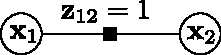
\includegraphics[width=0.2\textwidth]{pose_graph_1d_example.pdf}
    \end{figure}

    \small

    \begin{align*}
        \stateBold &=
        \begin{bmatrix}
            \stateBold_{1} & \stateBold_{2}
        \end{bmatrix}^{\top}
        =
        \begin{bmatrix}
            0 & 0
        \end{bmatrix}\\
        \observationBold_{12} &= 1\\
        \informationMatrix &= 2\\
        \error_{12} &= \observationBold_{12} - (\stateBold_{2} - \stateBold_{1}) = 1 - (0 - 0) = 1\\
        \jacobian_{12} &=
        \begin{bmatrix}
            1 & -1
        \end{bmatrix}\\
        \linearSystemb_{12}^{\top} &= \error_{12}^{\top} \informationMatrix_{12} \jacobian_{12} =
        \begin{bmatrix}
            2 & -2
        \end{bmatrix}\\
        \linearSystemH_{12} &= \jacobian_{12}^{\top} \informationMatrix_{12} \jacobian_{12} = 
        \begin{bmatrix}
            2 & -2\\
            -2 & 2
        \end{bmatrix}\\
    \vec{\Delta}\stateBold &= -\inverse{\linearSystemH}_{12} \linearSystemb_{12}\\
    \end{align*}

    \begin{center}
    \alert{Problema:} $\det(\linearSystemH) = 0$, por lo tanto no podemos invertir $\linearSystemH$
    \end{center}
\end{frame}

\begin{frame}
    \frametitle{¿Qué es lo que anda mal?}
    \note{Información extraída de https://youtu.be/uHbRKvD8TWg}
    
    \begin{itemize}
        \item La restricción especifica una restricción relativa entre ambos nodos
        \item Cualquier pose de los nodos va a estar bien si se cumple la restricción relativa entre ellos. Este problema se lo conoce como {\bf Gauge Freedom}
        \item Para resolverlo tenemos que {\bf fijar} un nodo. Al fijar un nodo estamos agregando un {\bf Prior}!
    \end{itemize}

    \begin{align*}
        \linearSystemH &=
        \begin{bmatrix}
            2 & -2\\
            -2 & 2
        \end{bmatrix}
        +
        \begin{bmatrix}
            1 & 0\\
            0 & 0
        \end{bmatrix} \leftarrow \text{restricción que pone } \vec{\Delta}\stateBold_{1} = 0\\
        \vec{\Delta}\stateBold &= -\inverse{\linearSystemH}_{12} \linearSystemb_{12}\\
        \vec{\Delta}\stateBold &=
        \begin{bmatrix}
            0 & 1
        \end{bmatrix}^{\top}
    \end{align*}
    
    Con esto hacemos que el update del nodo $\stateBold_{1}$ sea 0 y que el update de $\stateBold_{2}$ sea actualizado con 1.
\end{frame}

\begin{frame}
    \frametitle{Rol del Prior}
    \note{Información extraída de https://youtu.be/uHbRKvD8TWg}
    
    \begin{itemize}
        \item Vimos que la matriz de información $\linearSystemH$ no es de rango completa, y por tanto no es invertible
        \item Un marco de referencia global no ha sido fijado
        \item Fijar un marco de referencia global está fuertemente relacionado con el prior $p(\stateBold_{0})$
        \item Una estimación Gaussiana de $\stateBold_{0}$ resulta en agregar una restricción
        \item Ejemplo: La primera pose debe estar fija en el origen de coordenadas
        \begin{equation*}
            \error(\stateBold_{0}) = t2v(\stateBold_{0})
        \end{equation*}
    \end{itemize}
    
\end{frame}

\begin{frame}
    \frametitle{Fijando un subconjunto de variables}
    \note{Información extraída de https://youtu.be/uHbRKvD8TWg}
    
    \begin{itemize}
        \item Asumimos que el valor de ciertas variables durante la optimización es conocido a priori
        \item Queremos optimizar todos las demás variables pero manteniendo estas como fijas
        \item Podemos hacer como hicimos con el prior anterior, pero el problema es que es solo una {\bf soft constraint} y no es realmente un fix. Ya que puede suceder que otra constraint mueva a este nodo, y por tanto no podemos asegurar que tenga un valor fijo.
        \item Para efectivamente hacer que una variable quede fija, tenemos que hacer que no sea optimizada y por tanto debemos removerla del sistema lineal. Removerla del sistema lineal hace que no sea actualizada y que todas las demás variables esten restringidas por esta. Esto se hace construyendo todo el sistema lineal y luego sencillamente suprimiendo la fila y columna correspondiente a la variable. Finalmente se resuelve el sistema lineal.
        \item La supresión de la columna y fila funciona como una {\bf condicionamiento}, es decir, es una condición que dice ``Dado que un nodo toma un valor, las demás se ven afectadas de esta manera''
        
    \end{itemize}
    
\end{frame}

\begin{frame}
    \frametitle{Podemos suprimir las columnas y las filas de las variables correspondientes}
    \note{Información extraída de https://youtu.be/uHbRKvD8TWg}
    
    \begin{itemize}
        \item El porqué podemos hacer esto, resulta del {\bf condicionamiento de distribuciones Gaussianas}.
        \item {\bf Condicionamiento en el espacio de información}, significa que podemos remover una parte de la matriz de información y esto corresponde una operación de condicionamiento de la distribución Gaussiana.
        \item La $\linearSystemH$ es una matriz de información de todo nuestro problema con todas las restricciones juntas. Por tanto, removiendo una fila y una columna estamos condicionando al sistema haciendo que estas esten fijas y no se puedan actualizar y todas las demás variables queden restringidas por estas.
    \end{itemize}
   
    \footnotetext{Mas info en paper: Exactly sparse delayed-state filters for view-based SLAM. Eustice, Ryan M., Singh, Hanumant, Leonard, John J.}
    
\end{frame}

\begin{frame}
    \frametitle{Incertidumbre}
    \note{Información extraída de https://youtu.be/uHbRKvD8TWg}
    
    \begin{itemize}
        \item $\linearSystemH$ representa la matriz de información dado el punto de linearización
        \item La inversa de $\linearSystemH$ es la matriz de covarianza (densa). Calcular la inversa es muy costoso computacionalmente. Sin embargo, podemos computar partes de la matriz de covarianza.
        \item Los bloques de la diagonal de la matriz de covarianza representan las incertidumbres de las variables correspondientes
    \end{itemize}
\end{frame}

\begin{frame}
    \frametitle{Incertidumbre relativa}
    \note{Información extraída de https://youtu.be/uHbRKvD8TWg}
    
    Determinar la incertidumbre relativa entre $\stateBold_{i}$ y $\stateBold_{j}$.
    
    Esto es especialmente útil para la detección de ciclos, ya que podemos computar la incertidumbre de la pose actual con respecto a una pose anterior. De manera de poder determinar si es posible que haya un ciclo entre las poses o no (si la pose anterior se encuentra dentro de la covarianza entonces detectamos un ciclo).
    
    Para Determina la incertidumbre relativa entre $\stateBold_{i}$ y $\stateBold_{j}$ vamos a:    
    \begin{itemize}
        \item Construir la matriz completa $\linearSystemH$
        \item Suprimir las filas y columnas de $\stateBold_{i}$ (equivalente a no optimizar/fijar la variable)
        \item Computar el bloque $j,j$ de la inversa
        \item Este bloque contiene la matriz de covarianza de $\stateBold_{j}$ con respecto a $\stateBold_{i}$ la cuál está fija.
    \end{itemize}

    \begin{figure}[!h]
        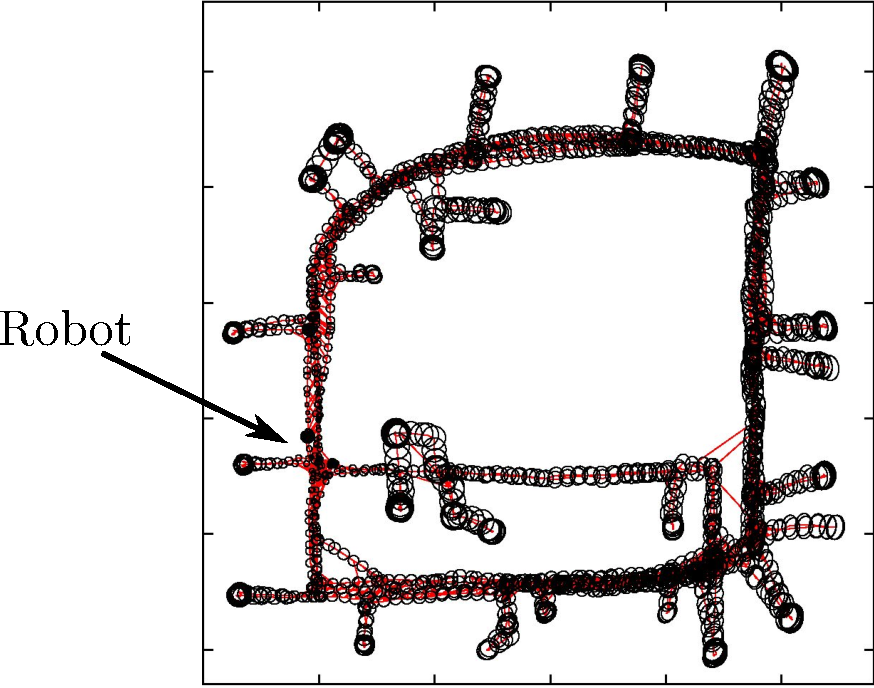
\includegraphics[width=0.2\textwidth]{pose_graph_relative_uncertainty.pdf}
    \end{figure}
    
\end{frame}

\begin{frame}
    \frametitle{Resumen de Pose-Graph}
    \note{Información extraída de https://youtu.be/uHbRKvD8TWg}
    
    \begin{itemize}
        \item El back-end del problema de SLAM puede ser resuelto aplicando Gauss-Newton
        \item La matriz $\linearSystemH$ es dispersa
        \item Que $\linearSystemH$ sea dispersa nos permite resolver el sistema lineal de manera eficiente
    \end{itemize}
    
\end{frame}

\begin{frame}
    \frametitle{Graph-Based SLAM con landmarks}
    \note{Información extraída de https://youtu.be/mZBdPgBtrCM}
    
       \begin{figure}[!h]
        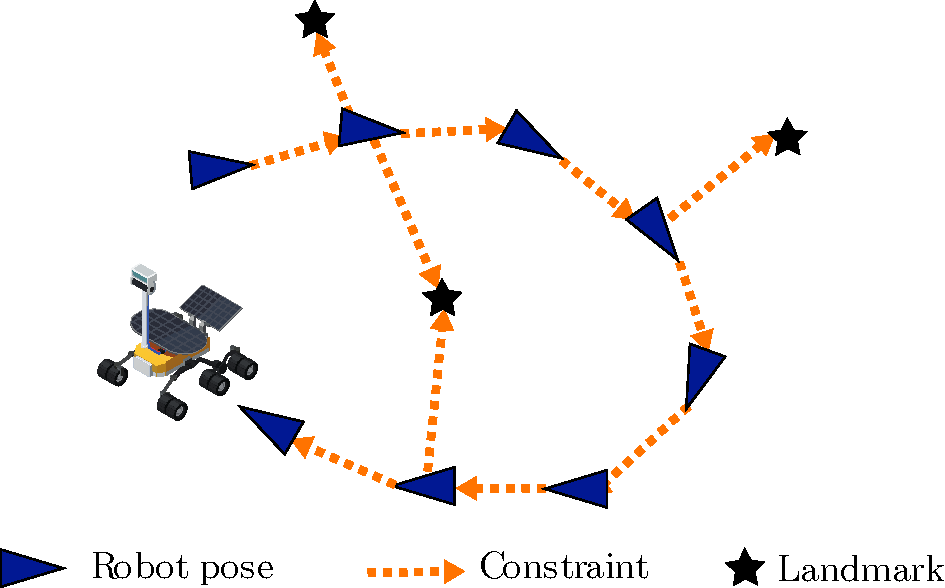
\includegraphics[width=0.6\textwidth]{images/pose_landmark_graph_example.pdf}
    \end{figure}
    
\end{frame}

\begin{frame}
    \frametitle{Observaciones de landmarks}
    \note{Información extraída de https://youtu.be/mZBdPgBtrCM}
    
    \begin{itemize}
        \item Observación esperada para un (x-y sensor\footnote{x-y sensor es un sensor cuyas mediciones tiene la forma (x,y), un punto de la escena. En un mundo 2D.})
           \begin{figure}[!h]
            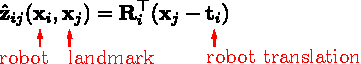
\includegraphics[width=0.6\textwidth]{images/pose_landmark_graph_expected_observation.pdf}
        \end{figure}
    \item Función error
    \begin{align*}
        \error_{ij}(\stateBold_{i}, \stateBold_{j}) &= \hat{\observationBold}_{ij} - \observationBold_{ij}\\
                    &= \rotation_{i}^{\top}(\stateBold_{j}-\translation_{i}) - \observationBold_{ij}
    \end{align*}
    \end{itemize}
    
\end{frame}

\begin{frame}
    \frametitle{Bearing only obsevations (observaciones de ángulo)}
    \note{Información extraída de https://youtu.be/mZBdPgBtrCM}
    
    \begin{itemize}
        \item Un landmark es un punto 2D
        \item El robot observa el ángulo hacia el landmark
        \item Función de observación
           \begin{figure}[!h]
            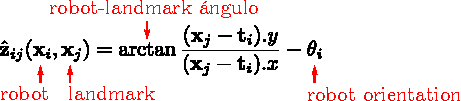
\includegraphics[width=0.6\textwidth]{images/pose_landmark_graph_bearing_observation.pdf}
        \end{figure}
        \item Función error
        \begin{equation*}
            \error_{ij}(\stateBold_{i},\stateBold_{j}) = \arctan{\dfrac{(\stateBold_{j}-\translation_{i}).y}{(\stateBold_{j}-\translation_{i}).x}} - \theta_{i} - \observationBold_{j}
        \end{equation*}
    \end{itemize}

    
\end{frame}

\begin{frame}
    \frametitle{Rango de la matriz H}
    \note{Información extraída de https://youtu.be/mZBdPgBtrCM}
    
    \TODO{Explicar bien cómo una medición restringe los parámetros a optimizar y cuantas mediciones son necesarias para estimar la pose y por qué.}
    
    \begin{itemize}
        \item ¿Cuál es el rango de la matriz $\linearSystemH_{ij}$ para una restricción pose-landmark 2D?
        \begin{itemize}
            \item El rango de $\linearSystemH_{ij}$ está determinado por el rango del Jacobiano $\jacobian_{ij}$ que a lo sumo es una matriz de $2 \times 5$ (2 porque la medición da información 2D y 5 por $\begin{bmatrix}    x & y & \theta & l_{x} & l_{y} \end{bmatrix}$)
            \item $\linearSystemH_{ij}$ no puede tener más que rango 2
            
                $rank(A^{\top} A) = rank(A^{\top}) = rank(A)$
        \end{itemize}
    
        \item ¿Cuál es el rango de la matriz $\linearSystemH_{ij}$ para una restricción pose-landmark bearing-only?
        \begin{itemize}
            \item El rango de $\linearSystemH_{ij}$ está determinado por el rango del Jacobiano $\jacobian_{ij}$ que a lo sumo es una matriz de $1 \times 5$. 1 porque la medición da información 1D y 5 por $\begin{bmatrix}    x & y & \theta & l_{x} & l_{y} \end{bmatrix}$
            \item $\linearSystemH_{ij}$ tiene rango 1
        \end{itemize}
        
    \end{itemize}
\end{frame}

\begin{frame}
    \frametitle{¿Dónde está el robot?}
    \note{Información extraída de https://youtu.be/mZBdPgBtrCM}
    \begin{itemize}
        \item El robot observa un landmark $(x,y)$
        \item ¿Dónde puede estar el robot relativo al landmark?
    \end{itemize}

    \only<1>{
        \begin{center}
            
\includegraphics[width=0.3\textwidth]{images/robot_pose_landmark_with_xy_sensor1.pdf}
        \end{center}
    }
    
    \only<2>{
        \begin{center}
            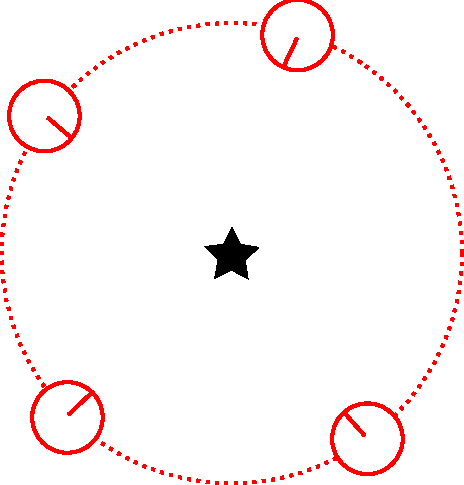
\includegraphics[width=0.3\textwidth]{images/robot_pose_landmark_with_xy_sensor2.pdf}
        \end{center}
        El robot puede estar en cualquier lugar del círculo.\\
        Es un espacio de soluciones 1D (restringido por la distancia y la orientación del robot)
    }
\end{frame}

\begin{frame}
    \frametitle{¿Dónde está el robot?}
    \note{Información extraída de https://youtu.be/mZBdPgBtrCM}
    \begin{itemize}
        \item El robot observa un landmark (bearing-only)
        \item ¿Dónde puede estar el robot relativo al landmark?
    \end{itemize}
    
    \only<1>{
        \begin{center}
            
\includegraphics[width=0.3\textwidth]{images/robot_pose_landmark_with_bearing_sensor1.pdf}
        \end{center}
    }
    
    \only<2>{
        \begin{center}
            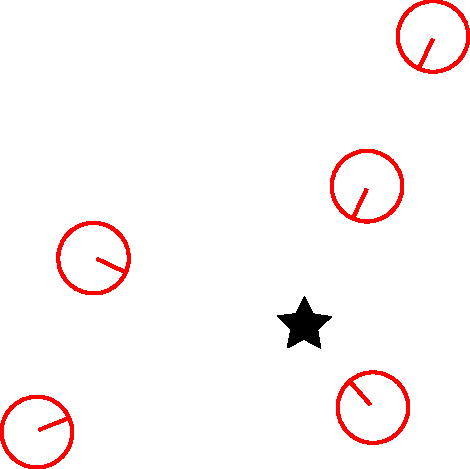
\includegraphics[width=0.3\textwidth]{images/robot_pose_landmark_with_bearing_sensor2.pdf}
        \end{center}
        El robot puede estar en cualquier lugar del plano xy. Siempre estará apuntando hacia el landmark.
        Es un espacio soluciones 2D (restringido por la orientación del robot).
    }
\end{frame}

\begin{frame}
    \frametitle{Rango}
    \note{Información extraída de https://youtu.be/mZBdPgBtrCM}
    \begin{itemize}
        \item En SLAM con landmarks, el sistema puede quedar indeterminado
        \item El rango de $\linearSystemH$ es {\bf menor o igual} que la suma de los rangos de todas las observaciones
        \item Para determinar una {\bf solución única}, el sistema debe tener {\bf rango completo}
    \end{itemize}
    \only<2>{
        Preguntas:
        \begin{itemize}
            \item ¿Cuantas observaciones de landmarks 2D se necesitan para resolver la pose de un robot?
            \item ¿Cuantas observaciones bearing-only se necesitan para resolver la pose de un robot?
        \end{itemize}
    }
\end{frame}

\begin{frame}
    \frametitle{Sistema indeterminado}
    \note{Información extraída de https://youtu.be/mZBdPgBtrCM}
    \begin{itemize}
        \item No hay garantía que que un sistema tenga rango completo
        \begin{itemize}
            \item Los landmarks puede ser observados una sola vez \TODO{no quedan claros estos items como influyen a la intederminación de H}
            \item El robot puede que no tenga información de odometría
        \end{itemize}
        \item Podemos lidiar con estos problemas utilizando un \emph{damping factor} para $\linearSystemH$
        \item En vez de resolver $\linearSystemH \vec{\Delta} \stateBold = - \linearSystemb$, resolvemos
        $(\linearSystemH + \lambda \vec{I}) \vec{\Delta} \stateBold = - \linearSystemb$
    \end{itemize}
\end{frame}

\begin{frame}
    \frametitle{Levenberg–Marquardt}
    \note{Información extraída de https://youtu.be/mZBdPgBtrCM}
    
    \footnotesize
    
    \begin{itemize}
        \item El damping factor $\lambda \vec{I}$ hace que el sistema sea definido positivo
        \item Es una suma ponderada del método de Gauss-Newton y el método de descenso por el gradiente \TODO{explicar bien esto, quizas con un grafico}
        \item El damping factor regula la convergencia usando acciones de backup/restore
    \end{itemize}

    \begin{algorithmic}[1]
        \Procedure{Levenberg–Marquardt}{$\stateBold$} \Comment{$\stateBold$: semilla inicial}
        \While (!converged)
        \State $\lambda =  \lambda_{\textrm{init}}$
        \State $<\linearSystemH, \linearSystemb> = buildLinearSystem(\stateBold)$
        \State $E = error(\stateBold)$
        \State $\stateBold_{\textrm{old}} = \stateBold$
        \State $\vec{\Delta}\stateBold = solveSparse((\linearSystemH + \lambda \vec{I}) \vec{\Delta} \stateBold = - \linearSystemb)$
        \State $\stateBold \mathrel{+}= \vec{\Delta}\stateBold$
        \If{$E < error(\stateBold)$}
        \State $\stateBold = \stateBold_{\textrm{old}}$
        \State $\lambda \mathrel{*}= 2$
        \Else
        \State $\lambda \mathrel{/}= 2$
        \EndIf
        \EndWhile
        \EndProcedure
    \end{algorithmic}

\end{frame}


	\section{EKF-SLAM}
	\begin{frame}
    \frametitle{Definición del Problema de SLAM}
    \note{Información extraída de https://www.youtube.com/watch?v=X30sEgIws0g}
    \note{Información extraída de https://www.ipb.uni-bonn.de/html/teaching/photo12-2021/2021-pho2-16-ekf-slam.pptx.pdf}

    Dado:
    \begin{itemize}
        \item Comandos de control enviados
        
        \begin{equation*}
            \controlCommand_{1:T} = \{\controlCommand_1, \controlCommand_2, \ldots, \controlCommand_T\}
        \end{equation*}
        \item Observaciones
        \begin{equation*}
            z_{1:T} = \{\observation_1, \observation_2, \ldots, \observation_T\}
        \end{equation*}
    \end{itemize}

    Se busca:
    \begin{itemize}
        \item Mapa del entorno: $\map$
        \item Trayectoria (o pose actual) del vehículo:
        \begin{equation*}
            \state_{0:T} = \{\state_0, \state_1, \ldots, \state_T\} \qquad \text{or} \qquad \state_{t}
        \end{equation*}
    \end{itemize}
\end{frame}

\begin{frame}
    \frametitle{Bayes Filter}
    \note{Información extraída de https://www.youtube.com/watch?v=X30sEgIws0g}
    \note{Información extraída de https://www.ipb.uni-bonn.de/html/teaching/photo12-2021/2021-pho2-16-ekf-slam.pptx.pdf}

    \begin{itemize}
        \item Recursive filter with \textbf{prediction} and \textbf{correction} steps
        \item Estimates: $p(x_t, \map | z_{1:t}, \controlCommand_{1:t})$
        \item Kalman Filter is a recursive Bayes Filter for the \textbf{linear Gaussian case}
        \item \textbf{EKF} for dealing with \textbf{non-linearities}
    \end{itemize}
\end{frame}

\begin{frame}
    \frametitle{Grafical Model of Full SLAM}
    \note{Información extraída de https://www.youtube.com/watch?v=X30sEgIws0g}
    \note{Información extraída de https://www.ipb.uni-bonn.de/html/teaching/photo12-2021/2021-pho2-16-ekf-slam.pptx.pdf}

    \[ p(\state_{1:t}, \map | z_{1:t}, \controlCommand_{1:t}) \]

    \begin{center}
        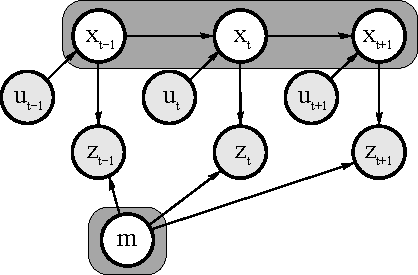
\includegraphics[width=0.6\textwidth]{../images/ekf_slam/graphical_model_full_slam.pdf}
    \end{center}
\end{frame}

\begin{frame}
    \frametitle{Grafical Model of Online SLAM}
    \note{Información extraída de https://www.youtube.com/watch?v=X30sEgIws0g}
    \note{Información extraída de https://www.ipb.uni-bonn.de/html/teaching/photo12-2021/2021-pho2-16-ekf-slam.pptx.pdf}

    We consider the Kalman filter as a solution to the online SLAM problem:
    \begin{equation*}
        p(\state_{t}, \map | z_{1:t}, \controlCommand_{1:t}) = \int \int \cdots \int p(\state_{1:t}, \map | z_{1:t}, \controlCommand_{1:t}) d\state_{1} d\state_{2} \ldots d\state_{t-1}
    \end{equation*}

    \begin{center}
        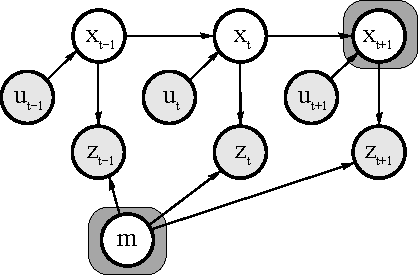
\includegraphics[width=0.6\textwidth]{../images/ekf_slam/graphical_model_online_slam.pdf}
    \end{center}
\end{frame}

\begin{frame}
    \frametitle{Algoritmo de Filtro de Kalman Extendido}
    \note{Información extraída de https://www.youtube.com/watch?v=X30sEgIws0g}
    \note{Información extraída de https://www.ipb.uni-bonn.de/html/teaching/photo12-2021/2021-pho2-16-ekf-slam.pptx.pdf}
    
    \begin{algorithmic}[1]
    \Procedure{ExtendedKalmanFilter}{$\mu_{t-1}, \covariance_{t-1}, \controlCommand_{t}, \observation_{t}$}
        \State $\overline{\mu}_{t} = \motionModelFunction{\controlCommand_{t}, \mu_{t-1}}$
        \State $\overline{\covariance}_{t} = \motionModelJacobian_{t} \covariance_{t-1} \motionModelJacobian_{t}^{\top}+\motionParametersCovariance_{t}$
        \Statex
        \State $\kalmanGain_{t} = \overline{\covariance}_{t} \observationModelJacobian_{t}^{\top} (\observationModelJacobian_{t} \overline{\covariance}_{t}  \observationModelJacobian_{t} + \observationModelCovariance_{t})^{-1} $
        \State $\mu_{t} = \overline{\mu}_{t} + \kalmanGain_{t} (\observation_{t} - \observationModelFunction{\overline{\mu}_{t}})$
        \State $\covariance_{t} =  (I - \kalmanGain_{t} \observationModelJacobian_{t}) \overline{\covariance}_{t}$
        \State \Return $\mu_{t}, \covariance_{t}$
    \EndProcedure
    \end{algorithmic}
\end{frame}

\begin{frame}
    \frametitle{EKF SLAM}
    \note{Información extraída de https://www.youtube.com/watch?v=X30sEgIws0g}
    \note{Información extraída de https://www.ipb.uni-bonn.de/html/teaching/photo12-2021/2021-pho2-16-ekf-slam.pptx.pdf}

    \begin{itemize}
        \item Application of EKF to SLAM
        \item Estimate robot's pose and landmark locations
        \item Assumption: known correspondences
        \item State space (2D plane):
    \end{itemize}
    \[ x_t = (x, y, \theta, \underbrace{\map_{1,x}, \map_{1,y}}_{\text{landmark 1}}, \ldots, \underbrace{\map_{n,x}, \map_{n,y}}_{\text{landmark n}} )^{\top} \]
\end{frame}

\begin{frame}
    \frametitle{EKF SLAM: State Representation}
    \note{Información extraída de https://www.youtube.com/watch?v=X30sEgIws0g}
    \note{Información extraída de https://www.ipb.uni-bonn.de/html/teaching/photo12-2021/2021-pho2-16-ekf-slam.pptx.pdf}

    \begin{itemize}
        \item Map with $n$ landmarks: $(3+2n)$-dimensional Gaussian
        \item Belief represented by:
        \begin{equation*}
            \underbrace{\begin{bNiceMatrix}[margin = 4pt]
                \CodeBefore
                \rectanglecolor{yellow!40}{1-1}{3-1}
                \rectanglecolor{blue!20}{4-1}{9-1}
                \Body
                x \\
                y \\
                \theta \\
                \map_{1,x} \\
                \map_{1,y} \\
                \vdots \\
                \map_{n,x} \\
                \map_{n,y}
            \end{bNiceMatrix}}_{\mu}
            \underbrace{\begin{bNiceMatrix}[margin = 4pt]
                \CodeBefore
                \rectanglecolor{yellow!40}{1-1}{3-3}
                \rectanglecolor{green!40}{1-4}{3-8}
                \rectanglecolor{green!40}{4-1}{8-3}
                \rectanglecolor{blue!20}{4-4}{8-8}
                \Body
                \sigma_{xx} & \sigma_{xy} & \sigma_{x\theta} & \sigma_{x \map_{1,x}} & \sigma_{x \map_{1,y}} & \cdots & \sigma_{x \map_{n,x}} & \sigma_{x \map_{n,y}}\\
                \sigma_{yx} & \sigma_{yy} & \sigma_{y\theta} & \sigma_{y \map_{1,x}} & \sigma_{y \map_{1,y}} & \cdots & \sigma_{y \map_{n,x}} & \sigma_{y \map_{n,y}}\\
                \sigma_{\theta x} & \sigma_{\theta y} & \sigma_{\theta\theta} & \sigma_{\theta \map_{1,x}} & \sigma_{\theta \map_{1,y}} & \cdots & \sigma_{\theta \map_{n,x}} & \sigma_{\theta \map_{n,y}}\\
                \sigma_{\map_{1,x}x} & \sigma_{\map_{1,x}y} & \sigma_{\map_{1,x}\theta} & \sigma_{\map_{1,x}\map_{1,x}} & \sigma_{\map_{1,x}\map_{1,y}} & \cdots & \sigma_{\map_{1,x} \map_{n,x}} & \sigma_{\map_{1,x} \map_{n,y}} \\
                \sigma_{\map_{1,y}x} & \sigma_{\map_{1,y}y} & \sigma_{\map_{1,y}\theta} & \sigma_{\map_{1,y}\map_{1,x}} & \sigma_{\map_{1,y}\map_{1,y}} & \cdots & \sigma_{\map_{1,y} \map_{n,x}} & \sigma_{\map_{1,y} \map_{n,y}} \\
                \vdots & \vdots & \vdots & \vdots & \vdots & \ddots & \vdots & \vdots \\
                \sigma_{\map_{n,x}x} & \sigma_{\map_{n,x}y} & \sigma_{\map_{n,x}\theta} & \sigma_{\map_{n,x} \map_{1,x}} & \sigma_{\map_{n,x} \map_{1,y}} &\cdots & \sigma_{\map_{n,x} \map_{n,x}} & \sigma_{\map_{n,x} \map_{n,y}} \\
                \sigma_{\map_{n,y}x} & \sigma_{\map_{n,y}y} & \sigma_{\map_{n,y}\theta} & \sigma_{\map_{n,y} \map_{1,x}} & \sigma_{\map_{n,y} \map_{1,y}} & \cdots & \sigma_{\map_{n,y} \map_{n,x}} & \sigma_{\map_{n,y} \map_{n,y}}
            \end{bNiceMatrix}}_{\Sigma}
        \end{equation*}
    \end{itemize}
\end{frame}

\begin{frame}
    \frametitle{EKF SLAM: State Representation}
    \note{Información extraída de https://www.youtube.com/watch?v=X30sEgIws0g}
    \note{Información extraída de https://www.ipb.uni-bonn.de/html/teaching/photo12-2021/2021-pho2-16-ekf-slam.pptx.pdf}

    \begin{itemize}
        \item Map with $n$ landmarks: $(3+2n)$-dimensional Gaussian
        \item Belief represented by:
        \begin{equation*}
            \underbrace{\begin{bNiceMatrix}[margin = 4pt]
                \CodeBefore
                \rectanglecolor{yellow!40}{1-1}{1-1}
                \rectanglecolor{blue!20}{2-1}{4-1}
                \Body
                \state_t \\
                \map_1 \\
                \vdots \\
                \map_n
            \end{bNiceMatrix}}_{\mu}
            \underbrace{\begin{bNiceMatrix}[margin = 4pt]
                \CodeBefore
                \rectanglecolor{yellow!40}{1-1}{1-1}
                \rectanglecolor{green!40}{2-1}{4-1}
                \rectanglecolor{green!40}{1-2}{1-4}
                \rectanglecolor{blue!20}{2-2}{4-4}
                \Body
                \Sigma_{\state_t \state_t} & \Sigma_{\state_t \map_1} & \cdots & \Sigma_{\state_t \map_n} \\
                \Sigma_{\map_1 \state_t} & \Sigma_{\map_1 \map_1} & \cdots & \Sigma_{\map_1 \map_n} \\
                \vdots & \vdots & \ddots & \vdots \\
                \Sigma_{\map_n \state_t} & \Sigma_{\map_n \map_1} & \cdots & \Sigma_{\map_n \map_n}
            \end{bNiceMatrix}}_{\Sigma}
        \end{equation*}
    \end{itemize}
\end{frame}

\begin{frame}
    \frametitle{EKF SLAM: State Representation}
    \note{Información extraída de https://www.youtube.com/watch?v=X30sEgIws0g}
    \note{Información extraída de https://www.ipb.uni-bonn.de/html/teaching/photo12-2021/2021-pho2-16-ekf-slam.pptx.pdf}

    \begin{itemize}
        \item More Compactly
        \begin{equation*}
            \underbrace{\begin{bNiceMatrix}[margin = 4pt]
                \CodeBefore
                \rectanglecolor{yellow!40}{1-1}{1-1}
                \rectanglecolor{blue!20}{2-1}{2-1}
                \Body
                \state\\
                \map
            \end{bNiceMatrix}}_{\mu}
            \underbrace{\begin{bNiceMatrix}[margin = 4pt]
                \CodeBefore
                \rectanglecolor{yellow!40}{1-1}{1-1}
                \rectanglecolor{green!40}{2-1}{2-1}
                \rectanglecolor{green!40}{1-2}{1-2}
                \rectanglecolor{blue!20}{2-2}{2-2}
                \Body
                \Sigma_{\state \state} & \Sigma_{\state \map} \\
                \Sigma_{\map \state} & \Sigma_{\map \map}
            \end{bNiceMatrix}}_{\Sigma}
        \end{equation*}
    \end{itemize}
\end{frame}

\begin{frame}
    \frametitle{EKF SLAM: Filter Cycle}
    \note{Información extraída de https://www.youtube.com/watch?v=X30sEgIws0g}
    \note{Información extraída de https://www.ipb.uni-bonn.de/html/teaching/photo12-2021/2021-pho2-16-ekf-slam.pptx.pdf}
    \begin{enumerate}
    \item State prediction
    \item Measurement prediction
    \item Measurement
    \item Data association
    \item Update
    \end{enumerate}
\end{frame}

\begin{frame}
    \frametitle{EKF SLAM: Initial State}
    \note{Información extraída de https://www.youtube.com/watch?v=X30sEgIws0g}
    \note{Información extraída de https://www.ipb.uni-bonn.de/html/teaching/photo12-2021/2021-pho2-16-ekf-slam.pptx.pdf}


    \begin{center}
        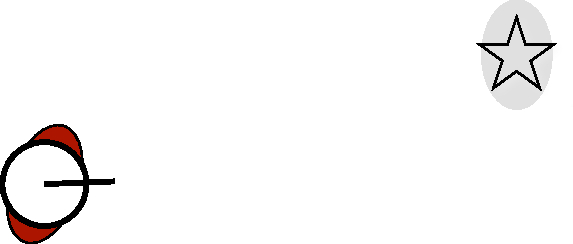
\includegraphics[width=0.5\textwidth]{./ekf_slam/ekf_slam_initial_state.pdf}
    \end{center}

    \begin{equation*}
        \underbrace{\begin{bNiceMatrix}
            \state_t \\
            \map_1 \\
            \vdots \\
            \map_n
        \end{bNiceMatrix}}_{\mu}
        \underbrace{\begin{bNiceMatrix}
            \Sigma_{\state_t \state_t} & \Sigma_{\state_t \map_1} & \cdots & \Sigma_{\state_t \map_n} \\
            \Sigma_{\map_1 \state_t} & \Sigma_{\map_1 \map_1} & \cdots & \Sigma_{\map_1 \map_n} \\
            \vdots & \vdots & \ddots & \vdots \\
            \Sigma_{\map_n \state_t} & \Sigma_{\map_n \map_1} & \cdots & \Sigma_{\map_n \map_n}
        \end{bNiceMatrix}}_{\Sigma}
    \end{equation*}
\end{frame}

\begin{frame}
    \frametitle{EKF SLAM: Predicted Motion}
    \note{Información extraída de https://www.youtube.com/watch?v=X30sEgIws0g}
    \note{Información extraída de https://www.ipb.uni-bonn.de/html/teaching/photo12-2021/2021-pho2-16-ekf-slam.pptx.pdf}


    \begin{center}
        \includegraphics[width=0.5\textwidth]{../images/ekf_slam/ekf_slam_predicted_motion.pdf}
    \end{center}

    \begin{equation*}
        \underbrace{\begin{bNiceMatrix}[margin = 4pt]
            \CodeBefore
            \rectanglecolor{green!40}{1-1}{1-1}
            \Body
            \state_t \\
            \map_1 \\
            \vdots \\
            \map_n
        \end{bNiceMatrix}}_{\mu}
        \underbrace{\begin{bNiceMatrix}[margin = 4pt]
            \CodeBefore
            \rectanglecolor{green!40}{1-1}{1-4}
            \rectanglecolor{green!40}{1-1}{4-1}
            \Body
            \Sigma_{\state_t \state_t} & \Sigma_{\state_t \map_1} & \cdots & \Sigma_{\state_t \map_n} \\
            \Sigma_{\map_1 \state_t} & \Sigma_{\map_1 \map_1} & \cdots & \Sigma_{\map_1 \map_n} \\
            \vdots & \vdots & \ddots & \vdots \\
            \Sigma_{\map_n \state_t} & \Sigma_{\map_n \map_1} & \cdots & \Sigma_{\map_n \map_n}
        \end{bNiceMatrix}}_{\Sigma}
    \end{equation*}
\end{frame}

\begin{frame}
    \frametitle{EKF SLAM: Predicted Measurement}
    \note{Información extraída de https://www.youtube.com/watch?v=X30sEgIws0g}
    \note{Información extraída de https://www.ipb.uni-bonn.de/html/teaching/photo12-2021/2021-pho2-16-ekf-slam.pptx.pdf}


    \begin{center}
        \includegraphics[width=0.5\textwidth]{../images/ekf_slam/ekf_slam_predicted_measurement.pdf}
    \end{center}

    \begin{equation*}
        \underbrace{\begin{bNiceMatrix}
            \state_t \\
            \map_1 \\
            \vdots \\
            \map_n
        \end{bNiceMatrix}}_{\mu}
        \underbrace{\begin{bNiceMatrix}
            \Sigma_{\state_t \state_t} & \Sigma_{\state_t \map_1} & \cdots & \Sigma_{\state_t \map_n} \\
            \Sigma_{\map_1 \state_t} & \Sigma_{\map_1 \map_1} & \cdots & \Sigma_{\map_1 \map_n} \\
            \vdots & \vdots & \ddots & \vdots \\
            \Sigma_{\map_n \state_t} & \Sigma_{\map_n \map_1} & \cdots & \Sigma_{\map_n \map_n}
        \end{bNiceMatrix}}_{\Sigma}
    \end{equation*}
\end{frame}

\begin{frame}
    \frametitle{EKF SLAM: Obtained Measurement}
    \note{Información extraída de https://www.youtube.com/watch?v=X30sEgIws0g}
    \note{Información extraída de https://www.ipb.uni-bonn.de/html/teaching/photo12-2021/2021-pho2-16-ekf-slam.pptx.pdf}


    \begin{center}
        \includegraphics[width=0.5\textwidth]{../images/ekf_slam/ekf_slam_obtained_measurement.pdf}
    \end{center}

    \begin{equation*}
        \underbrace{\begin{bNiceMatrix}
            \state_t \\
            \map_1 \\
            \vdots \\
            \map_n
        \end{bNiceMatrix}}_{\mu}
        \underbrace{\begin{bNiceMatrix}
            \Sigma_{\state_t \state_t} & \Sigma_{\state_t \map_1} & \cdots & \Sigma_{\state_t \map_n} \\
            \Sigma_{\map_1 \state_t} & \Sigma_{\map_1 \map_1} & \cdots & \Sigma_{\map_1 \map_n} \\
            \vdots & \vdots & \ddots & \vdots \\
            \Sigma_{\map_n \state_t} & \Sigma_{\map_n \map_1} & \cdots & \Sigma_{\map_n \map_n}
        \end{bNiceMatrix}}_{\Sigma}
    \end{equation*}
\end{frame}

\begin{frame}
    \frametitle{EKF SLAM: Data Association and Difference Between $h(x)$ and $\observation$}
    \note{Información extraída de https://www.youtube.com/watch?v=X30sEgIws0g}
    \note{Información extraída de https://www.ipb.uni-bonn.de/html/teaching/photo12-2021/2021-pho2-16-ekf-slam.pptx.pdf}

    \begin{center}
        \includegraphics[width=0.5\textwidth]{../images/ekf_slam/ekf_slam_difference_between_prediction_observation.pdf}
    \end{center}

    \begin{equation*}
        \underbrace{\begin{bNiceMatrix}
            \state_t \\
            \map_1 \\
            \vdots \\
            \map_n
        \end{bNiceMatrix}}_{\mu}
        \underbrace{\begin{bNiceMatrix}
            \Sigma_{\state_t \state_t} & \Sigma_{\state_t \map_1} & \cdots & \Sigma_{\state_t \map_n} \\
            \Sigma_{\map_1 \state_t} & \Sigma_{\map_1 \map_1} & \cdots & \Sigma_{\map_1 \map_n} \\
            \vdots & \vdots & \ddots & \vdots \\
            \Sigma_{\map_n \state_t} & \Sigma_{\map_n \map_1} & \cdots & \Sigma_{\map_n \map_n}
        \end{bNiceMatrix}}_{\Sigma}
    \end{equation*}
\end{frame}

\begin{frame}
    \frametitle{EKF SLAM: Update Step}
    \note{Información extraída de https://www.youtube.com/watch?v=X30sEgIws0g}
    \note{Información extraída de https://www.ipb.uni-bonn.de/html/teaching/photo12-2021/2021-pho2-16-ekf-slam.pptx.pdf}


    \begin{center}
        \includegraphics[width=0.5\textwidth]{../images/ekf_slam/ekf_slam_update.pdf}
    \end{center}

    \begin{equation*}
        \underbrace{\begin{bNiceMatrix}[margin = 4pt]
            \CodeBefore
            \rectanglecolor{green!40}{1-1}{4-1}
            \Body
            \state_t \\
            \map_1 \\
            \vdots \\
            \map_n
        \end{bNiceMatrix}}_{\mu}
        \underbrace{\begin{bNiceMatrix}[margin = 4pt]
            \CodeBefore
            \rectanglecolor{green!40}{1-1}{4-4}
            \Body
            \Sigma_{\state_t \state_t} & \Sigma_{\state_t \map_1} & \cdots & \Sigma_{\state_t \map_n} \\
            \Sigma_{\map_1 \state_t} & \Sigma_{\map_1 \map_1} & \cdots & \Sigma_{\map_1 \map_n} \\
            \vdots & \vdots & \ddots & \vdots \\
            \Sigma_{\map_n \state_t} & \Sigma_{\map_n \map_1} & \cdots & \Sigma_{\map_n \map_n}
        \end{bNiceMatrix}}_{\Sigma}
    \end{equation*}
\end{frame}

\begin{frame}
    \frametitle{EKF SLAM: Concrete Example}
    \note{Información extraída de https://www.youtube.com/watch?v=X30sEgIws0g}
    \note{Información extraída de https://www.ipb.uni-bonn.de/html/teaching/photo12-2021/2021-pho2-16-ekf-slam.pptx.pdf}

    Setup:
    \begin{itemize}
        \item Platform moves in the 2D plane
        \item Velocity-based motion model
        \item Observation of point landmarks
        \item Range-bearing sensor (measures distance and angle to landmarks)
        \item Known data association (which measurement comes from which landmark)
        \item Known number of landmarks
    \end{itemize}
\end{frame}

\begin{frame}
    \frametitle{Initialization}
    \note{Información extraída de https://www.youtube.com/watch?v=X30sEgIws0g}
    \note{Información extraída de https://www.ipb.uni-bonn.de/html/teaching/photo12-2021/2021-pho2-16-ekf-slam.pptx.pdf}

    \begin{itemize}
        \item Platform starts at the origin of its own reference frame
        \item All landmarks are initially unknown (not yet observed)
        \item State vector dimension: $2N + 3$ \\
        (3 for robot pose + $2N$ for $N$ landmarks in 2D space)
        \begin{equation*}
            \mu_0 =
            \begin{bmatrix}
                0 & 0 & 0 & \dots & 0    
            \end{bmatrix}^{\top}
        \end{equation*}
    \end{itemize}
    
    \begin{equation*}
        \Sigma_0 =
        \begin{bmatrix}
            \Sigma_{x_0} & 0 & \cdots & 0 \\
            0 & \infty I_{2} & \cdots & 0 \\
            \vdots & \vdots & \ddots & \vdots \\
            0 & 0 & \cdots & \infty I_{2}
        \end{bmatrix}
    \end{equation*}
    
    \begin{itemize}
        \item $\Sigma_{x_0}$: Initial uncertainty in robot pose (typically small)
        \item $\infty I_{2}$: Infinite uncertainty for unobserved landmarks
    \end{itemize}
\end{frame}

\begin{frame}
    \frametitle{Algoritmo de Filtro de Kalman Extendido}
    \note{Información extraída de https://www.youtube.com/watch?v=X30sEgIws0g}
    \note{Información extraída de https://www.ipb.uni-bonn.de/html/teaching/photo12-2021/2021-pho2-16-ekf-slam.pptx.pdf}
    
    \begin{algorithmic}[1]
    \Procedure{ExtendedKalmanFilter}{$\mu_{t-1}, \covariance_{t-1}, \controlCommand_{t}, \observation_{t}$}
        \State $\overline{\mu}_{t} = \alert{\motionModelFunction{\controlCommand_{t}, \mu_{t-1}}}$
        \State $\overline{\covariance}_{t} = \motionModelJacobian_{t} \covariance_{t-1} \motionModelJacobian_{t}^{\top}+\motionParametersCovariance_{t}$
        \Statex
        \State $\kalmanGain_{t} = \overline{\covariance}_{t} \observationModelJacobian_{t}^{\top} (\observationModelJacobian_{t} \overline{\covariance}_{t}  \observationModelJacobian_{t} + \observationModelCovariance_{t})^{-1} $
        \State $\mu_{t} = \overline{\mu}_{t} + \kalmanGain_{t} (\observation_{t} - \observationModelFunction{\overline{\mu}_{t}})$
        \State $\covariance_{t} =  (I - \kalmanGain_{t} \observationModelJacobian_{t}) \overline{\covariance}_{t}$
        \State \Return $\mu_{t}, \covariance_{t}$
    \EndProcedure
    \end{algorithmic}
\end{frame}

\begin{frame}
    \frametitle{Prediction Step (Motion)}
    \note{Información extraída de https://www.youtube.com/watch?v=X30sEgIws0g}
    \note{Información extraída de https://www.ipb.uni-bonn.de/html/teaching/photo12-2021/2021-pho2-16-ekf-slam.pptx.pdf}

    \begin{itemize}
        \item Goa: Update the state space based on the motion
        \item Motion in the plane (with a differential drive robot):
        \begin{equation*}
            \begin{bmatrix} x' \\ y' \\ \theta' \end{bmatrix} = 
            \underbrace{\begin{bmatrix} x \\ y \\ \theta \end{bmatrix} + 
            \begin{bmatrix} 
            -\frac{v_t}{\omega_t} \sin \theta + \frac{v_t}{\omega_t} \sin (\theta + \omega_t \Delta t) \\ 
            \frac{v_t}{\omega_t} \cos \theta - \frac{v_t}{\omega_t} \cos (\theta + \omega_t \Delta t) \\ 
            \omega_t \Delta t 
            \end{bmatrix}}_{g_{x,y,\theta}\left(\controlCommand_{t}, \begin{bmatrix} x, y, \theta \end{bmatrix}^{\top}\right)}
        \end{equation*}
        \item How to map that to the $2N+3$ dimmension state space used in EKF?
    \end{itemize}

\end{frame}

\begin{frame}
    \frametitle{Update the State Space}
    \note{Información extraída de https://www.youtube.com/watch?v=X30sEgIws0g}
    \note{Información extraída de https://www.ipb.uni-bonn.de/html/teaching/photo12-2021/2021-pho2-16-ekf-slam.pptx.pdf}

    \begin{itemize}
        \item From the motion in the plane
        
        \begin{equation*}
            \begin{bmatrix} x' \\ y' \\ \theta' \end{bmatrix} = 
            \underbrace{\begin{bmatrix} x \\ y \\ \theta \end{bmatrix} + 
            \begin{bmatrix} 
            -\frac{v_t}{\omega_t} \sin \theta + \frac{v_t}{\omega_t} \sin (\theta + \omega_t \Delta t) \\ 
            \frac{v_t}{\omega_t} \cos \theta - \frac{v_t}{\omega_t} \cos (\theta + \omega_t \Delta t) \\ 
            \omega_t \Delta t 
            \end{bmatrix}}_{g_{x,y,\theta}\left(\controlCommand_{t}, \begin{bmatrix} x, y, \theta \end{bmatrix}^{\top}\right)}
        \end{equation*}
    

        \item To the \(2N+3\) dimensional space:
        \begin{equation*}
            \begin{bmatrix}
            x' \\
            y' \\
            \theta'\\
            \vdots
            \end{bmatrix}
            =
            \underbrace{\begin{bmatrix}
            x \\
            y \\
            \theta\\
            \vdots
            \end{bmatrix}
            +
            \underbrace{\begin{bNiceMatrix}[margin = 3 pt]
            1 & 0 & 0 & 0 & \ldots & 0 \\
            0 & 1 & 0 & 0 & \ldots & 0 \\
            0 & 0 & 1 & 0 & \ldots & 0 \\
            & & & & &
            \CodeAfter
            \UnderBrace{3-4}{3-6}{2N cols}
            \end{bNiceMatrix}^{\top}}_{F_{x}^{\top}}
            \begin{bmatrix}
            -\frac{v_t}{\omega_t} \sin \theta + \frac{v_t}{\omega_t} \sin (\theta + \omega_t \Delta t) \\
            \frac{v_t}{\omega_t} \cos \theta - \frac{v_t}{\omega_t} \cos (\theta + \omega_t \Delta t) \\
            \omega_t \Delta t
            \end{bmatrix}}_{g(\controlCommand_{t}, \state_t)}
        \end{equation*}
    \end{itemize}
\end{frame}

\begin{frame}
    \frametitle{Algoritmo de Filtro de Kalman Extendido}
    \note{Información extraída de https://www.youtube.com/watch?v=X30sEgIws0g}
    \note{Información extraída de https://www.ipb.uni-bonn.de/html/teaching/photo12-2021/2021-pho2-16-ekf-slam.pptx.pdf}
    
    \begin{algorithmic}[1]
    \Procedure{ExtendedKalmanFilter}{$\mu_{t-1}, \covariance_{t-1}, \controlCommand_{t}, \observation_{t}$}
        \State $\overline{\mu}_{t} = \motionModelFunction{\controlCommand_{t}, \mu_{t-1}}$
        \State $\alert{\overline{\covariance}_{t} = \motionModelJacobian_{t} \covariance_{t-1} \motionModelJacobian_{t}^{\top}+\motionParametersCovariance_{t}}$
        \Statex
        \State $\kalmanGain_{t} = \overline{\covariance}_{t} \observationModelJacobian_{t}^{\top} (\observationModelJacobian_{t} \overline{\covariance}_{t}  \observationModelJacobian_{t} + \observationModelCovariance_{t})^{-1} $
        \State $\mu_{t} = \overline{\mu}_{t} + \kalmanGain_{t} (\observation_{t} - \observationModelFunction{\overline{\mu}_{t}})$
        \State $\covariance_{t} =  (I - \kalmanGain_{t} \observationModelJacobian_{t}) \overline{\covariance}_{t}$
        \State \Return $\mu_{t}, \covariance_{t}$
    \EndProcedure
    \end{algorithmic}
\end{frame}

\begin{frame}
    \frametitle{Update Covariance}
    \note{Información extraída de https://www.youtube.com/watch?v=X30sEgIws0g}
    \note{Información extraída de https://www.ipb.uni-bonn.de/html/teaching/photo12-2021/2021-pho2-16-ekf-slam.pptx.pdf}

    \begin{itemize}
        \item The function $g$ only affects de motion and not the landmarks
    \end{itemize}

    Jacobian:
    \begin{equation*}
        G_t = 
        \begin{bmatrix}
            G_{t}^{\state} & 0 \\
            0 & I
        \end{bmatrix}
    \end{equation*}
    where $G_t^x$ is the $3 \times 3$ Jacobian of the motion and $I$ is the $2N \times 2N$ identity matrix.
\end{frame}

\begin{frame}
    \frametitle{Jacobian of the Motion}
    \note{Información extraída de https://www.youtube.com/watch?v=X30sEgIws0g}
    \note{Información extraída de https://www.ipb.uni-bonn.de/html/teaching/photo12-2021/2021-pho2-16-ekf-slam.pptx.pdf}
    
    The Jacobian matrix \( G_t^x \) for the motion model is computed as:
    
    \begin{align*}
        G_t^x &= \frac{\partial}{\partial(x, y, \theta)^T} \left(
        \begin{bmatrix}
        x \\
        y \\
        \theta
        \end{bmatrix}
        +
        \begin{bmatrix}
        -\frac{v_t}{\omega_t} \sin \theta + \frac{v_t}{\omega_t} \sin(\theta + \omega_t \Delta t) \\
        \frac{v_t}{\omega_t} \cos \theta - \frac{v_t}{\omega_t} \cos(\theta + \omega_t \Delta t) \\
        \omega_t \Delta t
        \end{bmatrix}
        \right) \\
        &= I + \frac{\partial}{\partial(x, y, \theta)^T} 
        \begin{bmatrix}
        -\frac{v_t}{\omega_t} \sin \theta + \frac{v_t}{\omega_t} \sin(\theta + \omega_t \Delta t) \\
        \frac{v_t}{\omega_t} \cos \theta - \frac{v_t}{\omega_t} \cos(\theta + \omega_t \Delta t) \\
        \omega_t \Delta t
        \end{bmatrix} \\
        &= I + 
        \begin{bmatrix}
        0 & 0 & -\frac{v_t}{\omega_t} \cos \theta + \frac{v_t}{\omega_t} \cos(\theta + \omega_t \Delta t) \\
        0 & 0 & -\frac{v_t}{\omega_t} \sin \theta + \frac{v_t}{\omega_t} \sin(\theta + \omega_t \Delta t) \\
        0 & 0 & 0
        \end{bmatrix} \\
        &= 
        \begin{bmatrix}
        1 & 0 & -\frac{v_t}{\omega_t} \cos \theta + \frac{v_t}{\omega_t} \cos(\theta + \omega_t \Delta t) \\
        0 & 1 & -\frac{v_t}{\omega_t} \sin \theta + \frac{v_t}{\omega_t} \sin(\theta + \omega_t \Delta t) \\
        0 & 0 & 1
        \end{bmatrix}
    \end{align*}
    
\end{frame}

\begin{frame}
    \frametitle{This leads to the Covariance update}
    \note{Información extraída de https://www.youtube.com/watch?v=X30sEgIws0g}
    \note{Información extraída de https://www.ipb.uni-bonn.de/html/teaching/photo12-2021/2021-pho2-16-ekf-slam.pptx.pdf}

    \begin{align*}
        \bar{\Sigma}_t &= G_t \Sigma_{t-1} G_t^{\top} + R_t \\
        &= 
        \begin{bmatrix}
        G_t^x & 0 \\
        0 & I
        \end{bmatrix}
        \begin{bmatrix}
        \Sigma_{xx} & \Sigma_{xm} \\
        \Sigma_{mx} & \Sigma_{mm}
        \end{bmatrix}
        \begin{bmatrix}
        (G_t^x)^{\top} & 0 \\
        0 & I
        \end{bmatrix}
        + R_t \\
        &=
        \begin{bmatrix}
        G_t^x \Sigma_{xx} (G_t^x)^{\top} & G_t^x \Sigma_{xm} \\
        (G_t^x \Sigma_{xm})^{\top} & \Sigma_{mm}
        \end{bmatrix}
        + R_t
    \end{align*}

\end{frame}

\begin{frame}
    \frametitle{EKF SLAM: Prediction Step}
    \note{Información extraída de https://www.youtube.com/watch?v=X30sEgIws0g}
    \note{Información extraída de https://www.ipb.uni-bonn.de/html/teaching/photo12-2021/2021-pho2-16-ekf-slam.pptx.pdf}

    \begin{algorithmic}[1]
        \Procedure{EKF\_SLAM\_Prediction}{$\mu_{t-1}, \Sigma_{t-1}, \controlCommand_t, z_t, c_t, R_t$}
        \State $F_x = \begin{bmatrix}
        1 & 0 & 0 & 0 & 0 & \cdots & 0 \\
        0 & 1 & 0 & 0 & 0 & \cdots & 0 \\
        0 & 0 & 1 & 0 & 0 & \cdots & 0 \\
        \end{bmatrix}$
        \vspace{1em}
        \State $\bar{\mu}_t = \mu_{t-1} + F_x^{\top}
        \begin{bmatrix}
        \frac{-v_t}{\omega_t} \sin(\mu_{t-1,\theta}) + \frac{v_t}{\omega_t} \sin(\mu_{t-1,\theta} + \omega_t \Delta t) \\
        \frac{v_t}{\omega_t} \cos(\mu_{t-1,\theta}) - \frac{v_t}{\omega_t} \cos(\mu_{t-1,\theta} + \omega_t \Delta t) \\
        \omega_t \Delta t
        \end{bmatrix}$
        \vspace{1em}
        \State $G_t = I + F_x^{\top}
        \begin{bmatrix}
        0 & 0 & \frac{-v_t}{\omega_t} \cos(\mu_{t-1,\theta}) + \frac{v_t}{\omega_t} \cos(\mu_{t-1,\theta} + \omega_t \Delta t) \\
        0 & 0 & \frac{-v_t}{\omega_t} \sin(\mu_{t-1,\theta}) + \frac{v_t}{\omega_t} \sin(\mu_{t-1,\theta} + \omega_t \Delta t) \\
        0 & 0 & 0
        \end{bmatrix} F_x$
        \vspace{1em}
        \State $\bar{\Sigma}_t = G_t \Sigma_{t-1} G_t^{\top} + \underbrace{F_x^{\top} R_t F_x}_{R_t}$
        \EndProcedure
    \end{algorithmic}
    
\end{frame}

\begin{frame}
    \frametitle{Algoritmo de Filtro de Kalman Extendido}
    \note{Información extraída de https://www.youtube.com/watch?v=X30sEgIws0g}
    \note{Información extraída de https://www.ipb.uni-bonn.de/html/teaching/photo12-2021/2021-pho2-16-ekf-slam.pptx.pdf}
    
    \begin{algorithmic}[1]
    \Procedure{ExtendedKalmanFilter}{$\mu_{t-1}, \covariance_{t-1}, \controlCommand_{t}, \observation_{t}$}
        \State $\overline{\mu}_{t} = \motionModelFunction{\controlCommand_{t}, \mu_{t-1}}$
        \State $\overline{\covariance}_{t} = \motionModelJacobian_{t} \covariance_{t-1} \motionModelJacobian_{t}^{\top}+\motionParametersCovariance_{t}$
        \Statex
        \State $\alert{\kalmanGain_{t} = \overline{\covariance}_{t} \observationModelJacobian_{t}^{\top} (\observationModelJacobian_{t} \overline{\covariance}_{t}  \observationModelJacobian_{t} + \observationModelCovariance_{t})^{-1}}$
        \State $\alert{\mu_{t} = \overline{\mu}_{t} + \kalmanGain_{t} (\observation_{t} - \observationModelFunction{\overline{\mu}_{t}})}$
        \State $\alert{\covariance_{t} =  (I - \kalmanGain_{t} \observationModelJacobian_{t}) \overline{\covariance}_{t}}$
        \State \Return $\mu_{t}, \covariance_{t}$
    \EndProcedure
    \end{algorithmic}
\end{frame}

\begin{frame}
    \frametitle{EKF SLAM: Correction Step}
    \note{Información extraída de https://www.youtube.com/watch?v=X30sEgIws0g}
    \note{Información extraída de https://www.ipb.uni-bonn.de/html/teaching/photo12-2021/2021-pho2-16-ekf-slam.pptx.pdf}

    \begin{itemize}
        \item Known data association
        \item $c_{t}^{i} = j$ : $i$-th measurement at time $t$ observes the landmark with index $j$
        \item Initialize landmark if unobserved
        \item Compute the expected observation
        \item Compute the Jacobian of $h$
        \item Proceed with computing the Kalman gain
    \end{itemize}

\end{frame}

\begin{frame}
    \frametitle{Algoritmo de Filtro de Kalman Extendido}
    \note{Información extraída de https://www.youtube.com/watch?v=X30sEgIws0g}
    \note{Información extraída de https://www.ipb.uni-bonn.de/html/teaching/photo12-2021/2021-pho2-16-ekf-slam.pptx.pdf}
    
    \begin{algorithmic}[1]
    \Procedure{ExtendedKalmanFilter}{$\mu_{t-1}, \covariance_{t-1}, \controlCommand_{t}, \observation_{t}$}
        \State $\overline{\mu}_{t} = \motionModelFunction{\controlCommand_{t}, \mu_{t-1}}$
        \State $\overline{\covariance}_{t} = \motionModelJacobian_{t} \covariance_{t-1} \motionModelJacobian_{t}^{\top}+\motionParametersCovariance_{t}$
        \Statex
        \State $\kalmanGain_{t} = \overline{\covariance}_{t} \alert{\observationModelJacobian_{t}^{\top}} (\observationModelJacobian_{t} \overline{\covariance}_{t}  \observationModelJacobian_{t} + \observationModelCovariance_{t})^{-1} $
        \State $\mu_{t} = \overline{\mu}_{t} + \kalmanGain_{t} (\observation_{t} - \observationModelFunction{\overline{\mu}_{t}})$
        \State $\covariance_{t} =  (I - \kalmanGain_{t} \observationModelJacobian_{t}) \overline{\covariance}_{t}$
        \State \Return $\mu_{t}, \covariance_{t}$
    \EndProcedure
    \end{algorithmic}
\end{frame}

\begin{frame}
    \frametitle{Range-Bearing Observation}
    \note{Información extraída de https://www.youtube.com/watch?v=X30sEgIws0g}
    \note{Información extraída de https://www.ipb.uni-bonn.de/html/teaching/photo12-2021/2021-pho2-16-ekf-slam.pptx.pdf}

    \begin{itemize}
        \item Range-Bearing observation $z_t^i = \begin{bmatrix} r_t^i \\ \phi_t^i \end{bmatrix}^{\top}$
        
        \item If landmark has not been observed, we can initialize it with:
    \end{itemize}
    
    \begin{equation*}
        \underbrace{
        \begin{bmatrix}
        \bar{\mu}_{j,x} \\
        \bar{\mu}_{j,y}
        \end{bmatrix}}_{\parbox{2cm}{\centering \scriptsize \text{location of} \\ \text{landmark} j}}
        =
        \underbrace{
        \begin{bmatrix}
        \bar{\mu}_{t,x} \\
        \bar{\mu}_{t,y}
        \end{bmatrix}}_{\parbox{2cm}{\centering \scriptsize \text{estimated location} \\ \text{of the platform}}}
        +
        \underbrace{
        \begin{bmatrix}
        r_t^i \cos(\phi_t^i + \bar{\mu}_{t,\theta}) \\
        r_t^i \sin(\phi_t^i + \bar{\mu}_{t,\theta})
        \end{bmatrix}}_{\text{relative measurement}}
    \end{equation*}
\end{frame}

\begin{frame}
    \frametitle{Expected Observation: $h(x)$}
    \note{Información extraída de https://www.youtube.com/watch?v=X30sEgIws0g}
    \note{Información extraída de https://www.ipb.uni-bonn.de/html/teaching/photo12-2021/2021-pho2-16-ekf-slam.pptx.pdf}

    \begin{itemize}
        \item Compute expected observation according to the current estimate 
    \end{itemize}

    \begin{align*}
        \delta &= \begin{bmatrix}
        \delta_x \\
        \delta_y
        \end{bmatrix} = \begin{bmatrix}
        \bar{\mu}_{j,x} - \bar{\mu}_{t,x} \\
        \bar{\mu}_{j,y} - \bar{\mu}_{t,y}
        \end{bmatrix}\\
        q &= \delta^{\top} \delta\\
        \hat{z}_t^i &= \begin{bmatrix}
        \sqrt{q} \\
        \text{atan2}(\delta_y, \delta_x) - \bar{\mu}_{t,\theta}
        \end{bmatrix}\\
        &= h(\bar{\mu}_t)
    \end{align*}
\end{frame}

\begin{frame}
    \frametitle{Jacobian for the Observation}
    \note{Información extraída de https://www.youtube.com/watch?v=X30sEgIws0g}
    \note{Información extraída de https://www.ipb.uni-bonn.de/html/teaching/photo12-2021/2021-pho2-16-ekf-slam.pptx.pdf}

    \begin{itemize}
        \item Based on
        \begin{align*}
            \delta &= 
            \begin{bmatrix}
                \delta_x \\
                \delta_y
            \end{bmatrix}
            = \begin{bmatrix}
                \bar{\mu}_{j,x} - \bar{\mu}_{t,x} \\
                \bar{\mu}_{j,y} - \bar{\mu}_{t,y}
            \end{bmatrix}\\
            q &= \delta^T \delta\\
            \hat{z}^i_t &= 
            \begin{bmatrix}
                \sqrt{q} \\
                \text{atan2}(\delta_y, \delta_x) - \bar{\mu}_{t,\theta}
            \end{bmatrix}
        \end{align*}    
        \item Compute the Jacobian
        \begin{equation*}
            \prescript{\text{low}}{}{H^{i}_{t}} = \frac{\partial h(\bar{\mu}_t)}{\partial \bar{\mu}_t}
        \end{equation*}
        \begin{equation*}
            \text{low-dim space} \quad (x, y, \theta, \map{j,x}, \map{j,y})
        \end{equation*}
    \end{itemize}
\end{frame}

\begin{frame}
    \frametitle{Jacobian for the Observation}
    \note{Información extraída de https://www.youtube.com/watch?v=X30sEgIws0g}
    \note{Información extraída de https://www.ipb.uni-bonn.de/html/teaching/photo12-2021/2021-pho2-16-ekf-slam.pptx.pdf}

    \begin{itemize}
        \item Based on
        \begin{align*}
            \delta &= 
            \begin{bmatrix}
                \delta_x \\
                \delta_y
            \end{bmatrix}
            = \begin{bmatrix}
                \bar{\mu}_{j,x} - \bar{\mu}_{t,x} \\
                \bar{\mu}_{j,y} - \bar{\mu}_{t,y}
            \end{bmatrix}\\
            q &= \delta^T \delta\\
            \hat{z}^i_t &= 
            \begin{bmatrix}
                \sqrt{q} \\
                \text{atan2}(\delta_y, \delta_x) - \bar{\mu}_{t,\theta}
            \end{bmatrix}
        \end{align*}    
        \item Compute the Jacobian
        \begin{align*}
            \prescript{\text{low}}{}{H^{i}_{t}} &= \frac{\partial h(\bar{\mu}_t)}{\partial \bar{\mu}_t}\\
            &= \begin{bmatrix}
                \frac{\partial \sqrt{q}}{\partial x} & \frac{\partial \sqrt{q}}{\partial y} & \cdots \\
                \frac{\partial \text{atan2}(\ldots)}{\partial x} & \frac{\partial \text{atan2}(\ldots)}{\partial y} & \cdots
            \end{bmatrix}
    \end{align*} 
    \end{itemize}

\end{frame}

\begin{frame}
    \frametitle{The first component}
    \note{Información extraída de https://www.youtube.com/watch?v=X30sEgIws0g}
    \note{Información extraída de https://www.ipb.uni-bonn.de/html/teaching/photo12-2021/2021-pho2-16-ekf-slam.pptx.pdf}

    \begin{itemize}
        \item Based on
        \begin{align*}
            \delta &= 
            \begin{bmatrix}
                \delta_x \\
                \delta_y
            \end{bmatrix}
            = \begin{bmatrix}
                \bar{\mu}_{j,x} - \bar{\mu}_{t,x} \\
                \bar{\mu}_{j,y} - \bar{\mu}_{t,y}
            \end{bmatrix}\\
            q &= \delta^T \delta\\
            \hat{z}^i_t &= 
            \begin{bmatrix}
                \sqrt{q} \\
                \text{atan2}(\delta_y, \delta_x) - \bar{\mu}_{t,\theta}
            \end{bmatrix}
        \end{align*}    
    
        \item We obtain (by applying the chain rule)
        \begin{align*}
            \frac{\partial \sqrt{q}}{\partial x}
            &= \frac{1}{2} \cdot \frac{1}{\sqrt{q}} \cdot 2 \delta_x \cdot (-1)\\
            &= \frac{1}{q} \left(-\sqrt{q} \delta_x \right)
        \end{align*} 
    \end{itemize}

\end{frame}

\begin{frame}
    \frametitle{Jacobian for the Observation}
    \note{Información extraída de https://www.youtube.com/watch?v=X30sEgIws0g}
    \note{Información extraída de https://www.ipb.uni-bonn.de/html/teaching/photo12-2021/2021-pho2-16-ekf-slam.pptx.pdf}

    \begin{itemize}
        \item Based on
        \begin{align*}
            \delta &= 
            \begin{bmatrix}
                \delta_x \\
                \delta_y
            \end{bmatrix}
            = \begin{bmatrix}
                \bar{\mu}_{j,x} - \bar{\mu}_{t,x} \\
                \bar{\mu}_{j,y} - \bar{\mu}_{t,y}
            \end{bmatrix}\\
            q &= \delta^T \delta\\
            \hat{z}^i_t &= 
            \begin{bmatrix}
                \sqrt{q} \\
                \text{atan2}(\delta_y, \delta_x) - \bar{\mu}_{t,\theta}
            \end{bmatrix}
        \end{align*}

        \item Compute the Jacobian
        
        \begin{align*}
            \prescript{\text{low}}{}{H^{i}_{t}} &= \frac{\partial h(\bar{\mu}_t)}{\partial \bar{\mu}_t}\\
            &= \frac{1}{q}
            \begin{bmatrix}
                -\sqrt{q} \delta_x & -\sqrt{q} \delta_y & 0 & \sqrt{q} \delta_x & \sqrt{q} \delta_y\\
                \delta_y & -\delta_x & -q & -\delta_y & \delta_x
            \end{bmatrix}
        \end{align*}
    \end{itemize}

\end{frame}

\begin{frame}
    \frametitle{Jacobian for the Observation}
    \note{Información extraída de https://www.youtube.com/watch?v=X30sEgIws0g}
    \note{Información extraída de https://www.ipb.uni-bonn.de/html/teaching/photo12-2021/2021-pho2-16-ekf-slam.pptx.pdf}

    \small

    \begin{itemize}
        \item Use the computed Jacobian
        \begin{align*}
            \prescript{\text{low}}{}{H^{i}_{t}} &= \frac{\partial h(\bar{\mu}_t)}{\partial \bar{\mu}_t}\\
            &= \frac{1}{q}
            \begin{bmatrix}
                -\sqrt{q} \delta_x & -\sqrt{q} \delta_y & 0 & \sqrt{q} \delta_x & \sqrt{q} \delta_y\\
                \delta_y & -\delta_x & -q & -\delta_y & \delta_x
            \end{bmatrix}
        \end{align*}
    
        \item Map it to the high dimensional space
        \begin{equation*}
            H^{i}_{t} = \prescript{\text{low}}{}{H^{i}_{t}} F_{x,j}
        \end{equation*}
        \begin{equation*}
            F_{x,j} =
            \begin{bNiceMatrix}[margin = 3 pt]
                1 & 0 & 0 & 0 \cdots 0 & 0 & 0 & 0 \cdots 0 \\
                0 & 1 & 0 & 0 \cdots 0 & 0 & 0 & 0 \cdots 0 \\
                0 & 0 & 1 & 0 \cdots 0 & 0 & 0 & 0 \cdots 0 \\
                0 & 0 & 0 & 0 \cdots 0 & 1 & 0 & 0 \cdots 0 \\
                0 & 0 & 0 & 0 \cdots 0 & 0 & 1 & 0 \cdots 0
                \CodeAfter
                \UnderBrace{5-4}{5-4}{2j-2}
                \UnderBrace{5-7}{5-7}{2N-2j}
            \end{bNiceMatrix}
        \end{equation*} 
    \end{itemize}
\end{frame}

\begin{frame}
    \frametitle{Algoritmo de Filtro de Kalman Extendido}
    \note{Información extraída de https://www.youtube.com/watch?v=X30sEgIws0g}
    \note{Información extraída de https://www.ipb.uni-bonn.de/html/teaching/photo12-2021/2021-pho2-16-ekf-slam.pptx.pdf}
    
    \begin{algorithmic}[1]
    \Procedure{ExtendedKalmanFilter}{$\mu_{t-1}, \covariance_{t-1}, \controlCommand_{t}, \observation_{t}$}
        \State $\overline{\mu}_{t} = \motionModelFunction{\controlCommand_{t}, \mu_{t-1}}$
        \State $\overline{\covariance}_{t} = \motionModelJacobian_{t} \covariance_{t-1} \motionModelJacobian_{t}^{\top}+\motionParametersCovariance_{t}$
        \Statex
        \State $\alert{\kalmanGain_{t} = \overline{\covariance}_{t} \observationModelJacobian_{t}^{\top} (\observationModelJacobian_{t} \overline{\covariance}_{t}  \observationModelJacobian_{t} + \observationModelCovariance_{t})^{-1}}$
        \State $\alert{\mu_{t} = \overline{\mu}_{t} + \kalmanGain_{t} (\observation_{t} - \observationModelFunction{\overline{\mu}_{t}})}$
        \State $\alert{\covariance_{t} =  (I - \kalmanGain_{t} \observationModelJacobian_{t}) \overline{\covariance}_{t}}$
        \State \Return $\mu_{t}, \covariance_{t}$
    \EndProcedure
    \end{algorithmic}
\end{frame}

\begin{frame}
    \frametitle{EKF SLAM - Correction (1/2)}
    \note{Información extraída de https://www.youtube.com/watch?v=X30sEgIws0g}
    \note{Información extraída de https://www.ipb.uni-bonn.de/html/teaching/photo12-2021/2021-pho2-16-ekf-slam.pptx.pdf}

    \begin{algorithmic}[1]
        \Procedure{EKF\_SLAM\_Correction}{}
        \State $Q_t = \begin{bmatrix} \sigma_r^2 & 0 \\ 0 & \sigma_\theta^2 \end{bmatrix}$ \Comment{Measurement noise covariance}
        \For {all observed features $z_i^t = (r_i^t, \phi_i^t)^{\top}$}
            \State $j = c_i^t$ \Comment{Landmark identifier}
            \If{landmark $j$ never seen before}
                \State $\begin{bmatrix} \bar{\mu}_{j,x} \\ \bar{\mu}_{j,y} \end{bmatrix} = 
                       \begin{bmatrix} \bar{\mu}_{t,x} \\ \bar{\mu}_{t,y} \end{bmatrix} + 
                       \begin{bmatrix} r_i^t \cos(\phi_i^t + \bar{\mu}_{t,\theta}) \\ r_i^t \sin(\phi_i^t + \bar{\mu}_{t,\theta}) \end{bmatrix}$
                \Comment{Initialize new landmark position}
            \EndIf
            \State $\delta = \begin{bmatrix} \delta_x \\ \delta_y \end{bmatrix} = 
                   \begin{bmatrix} \bar{\mu}_{j,x} - \bar{\mu}_{t,x} \\ \bar{\mu}_{j,y} - \bar{\mu}_{t,y} \end{bmatrix}$
            \State $q = \delta^T \delta$
            \State $\hat{z}_i^t = \begin{bmatrix} \sqrt{q} \\ \operatorname{atan2}(\delta_y, \delta_x) - \bar{\mu}_{t,\theta} \end{bmatrix}$
                   \Comment{Predicted measurement}
        \algstore{ekf_slam_algorithm_break} % guarda el estado del argoritmo para que este pueda continuar en otro lugar
    \end{algorithmic}
\end{frame}

\begin{frame}
    \frametitle{EKF SLAM - Correction (2/2)}
    \note{Información extraída de https://www.youtube.com/watch?v=X30sEgIws0g}
    \note{Información extraída de https://www.ipb.uni-bonn.de/html/teaching/photo12-2021/2021-pho2-16-ekf-slam.pptx.pdf}

    \begin{algorithmic}[1]
        \algrestore{ekf_slam_algorithm_break} % continua el algoritmo de antes
        \State $F_{x,j} =
        \begin{bNiceMatrix}[margin = 3 pt]
            1 & 0 & 0 & 0 \cdots 0 & 0 & 0 & 0 \cdots 0 \\
            0 & 1 & 0 & 0 \cdots 0 & 0 & 0 & 0 \cdots 0 \\
            0 & 0 & 1 & 0 \cdots 0 & 0 & 0 & 0 \cdots 0 \\
            0 & 0 & 0 & 0 \cdots 0 & 1 & 0 & 0 \cdots 0 \\
            0 & 0 & 0 & 0 \cdots 0 & 0 & 1 & 0 \cdots 0
            \CodeAfter
            \UnderBrace{5-4}{5-4}{2j-2}
            \UnderBrace{5-7}{5-7}{2N-2j}
        \end{bNiceMatrix}$ \Comment{Jacobian of state mapping}
        \Statex
        \Statex
        \State $H_t^i = \frac{1}{q} \begin{bmatrix}
            -\sqrt{q} \delta_x & -\sqrt{q} \delta_y & 0 & \sqrt{q} \delta_x & \sqrt{q} \delta_y\\
            \delta_y & -\delta_x & -q & -\delta_y & \delta_x
        \end{bmatrix} F_{x,j}$ \Comment{Measurement Jacobian}
            
        \State $K_t^i = \bar{\Sigma}_t H_t^{i\top}(H_t^i \bar{\Sigma}_t H_t^{i\top} + Q_t)^{-1}$ \Comment{Kalman gain}
        \State $\bar{\mu}_t = \bar{\mu}_t + K_t^i(z_t^i - \hat{z}_t^i)$ \Comment{State update}
        \State $\bar{\Sigma}_t = (I - K_t^i H_t^i) \bar{\Sigma}_t$ \Comment{Covariance update}
        \EndFor
        \State $\mu_t = \bar{\mu}_t$ \Comment{Final state estimate}
        \State $\Sigma_t = \bar{\Sigma}_t$ \Comment{Final covariance estimate}
        \State \Return $\mu_t, \Sigma_t$ \Comment{Return updated state and covariance}
        \EndProcedure
    \end{algorithmic}
\end{frame}

\begin{frame}
    \frametitle{Implementation Notes}
    \note{Información extraída de https://www.youtube.com/watch?v=X30sEgIws0g}
    \note{Información extraída de https://www.ipb.uni-bonn.de/html/teaching/photo12-2021/2021-pho2-16-ekf-slam.pptx.pdf}

    \begin{itemize}
    \item Measurement update in a single step requires only one full belief update
    \item Always normalize angular components
    \item May not need to create $F$ matrices explicitly
    \end{itemize}
\end{frame}

\begin{frame}
    \frametitle{Loop Closing}
    \note{Información extraída de https://www.youtube.com/watch?v=X30sEgIws0g}
    \note{Información extraída de https://www.ipb.uni-bonn.de/html/teaching/photo12-2021/2021-pho2-16-ekf-slam.pptx.pdf}

    \begin{itemize}
    \item Loop closing means revisiting (and recognizing) an already mapped area
    \item Data association under
    \begin{itemize}
        \item high ambiguity
        \item possible environment symmetries
    \end{itemize}
    \item Uncertainties collapse after a loop closure (whether the closure was correct or not) 
    \end{itemize}
\end{frame}

\begin{frame}
    \frametitle{Before the Loop Closure}
    \note{Información extraída de https://www.youtube.com/watch?v=X30sEgIws0g}
    \note{Información extraída de https://www.ipb.uni-bonn.de/html/teaching/photo12-2021/2021-pho2-16-ekf-slam.pptx.pdf}

    \begin{center}
        \includegraphics[width=0.6\textwidth]{ekf_slam/ekf_slam_loop_closure_before.pdf}
    \end{center}
\end{frame}

\begin{frame}
    \frametitle{After the Loop Closure}
    \note{Información extraída de https://www.youtube.com/watch?v=X30sEgIws0g}
    \note{Información extraída de https://www.ipb.uni-bonn.de/html/teaching/photo12-2021/2021-pho2-16-ekf-slam.pptx.pdf}

    \begin{center}
        \includegraphics[width=0.6\textwidth]{ekf_slam/ekf_slam_loop_closure_after.pdf}
    \end{center}
\end{frame}

\begin{frame}
    \frametitle{Loop Closing}
    \note{Información extraída de https://www.youtube.com/watch?v=X30sEgIws0g}
    \note{Información extraída de https://www.ipb.uni-bonn.de/html/teaching/photo12-2021/2021-pho2-16-ekf-slam.pptx.pdf}

    \begin{itemize}
    \item Loop closing reduces the uncertainty in robot and landmark estimates
    \item This can be exploited when exploring an environment for the sake of better (e.g. more accurate) maps
    \item Wrong loop closures lead to filter divergence
    \end{itemize}
\end{frame}

\begin{frame}
    \frametitle{EKF SLAM Correlations}
    \note{Información extraída de https://www.youtube.com/watch?v=X30sEgIws0g}
    \note{Información extraída de https://www.ipb.uni-bonn.de/html/teaching/photo12-2021/2021-pho2-16-ekf-slam.pptx.pdf}

    \begin{itemize}
        \item In the limit, the landmark estimates become fully correlated
    \end{itemize}

    \begin{center}
        \includegraphics[width=0.5\textwidth]{../images/ekf_slam/ekf_slam_correlations.pdf}
    \end{center}

    \begin{itemize}
        \item The Covariance Matrix represents the uncertainty and correlation between different state variables (e.g., robot pose at different time steps and positions of landmarks).
        \begin{itemize}
            \item Diagonal: Variance (uncertainty) of each variable.
            \item Off-diagonal: Correlation between variables (how errors in one affect another).
        \end{itemize}
    \end{itemize}
    
\end{frame}

\begin{frame}
    \frametitle{EKF SLAM Correlations}
    \note{Información extraída de https://www.youtube.com/watch?v=X30sEgIws0g}
    \note{Información extraída de https://www.ipb.uni-bonn.de/html/teaching/photo12-2021/2021-pho2-16-ekf-slam.pptx.pdf}

    \begin{center}
        \only<1>{\includegraphics[width=0.8\textwidth]{../images/ekf_slam/ekf_slam_correlation_matrix1.pdf}}
        \only<2>{\includegraphics[width=0.8\textwidth]{../images/ekf_slam/ekf_slam_correlation_matrix2.pdf}}
        \only<3>{\includegraphics[width=0.8\textwidth]{../images/ekf_slam/ekf_slam_correlation_matrix3.pdf}}
    \end{center}
\end{frame}

\begin{frame}
    \frametitle{EKF SLAM Correlations}
    \note{Información extraída de https://www.youtube.com/watch?v=X30sEgIws0g}
    \note{Información extraída de https://www.ipb.uni-bonn.de/html/teaching/photo12-2021/2021-pho2-16-ekf-slam.pptx.pdf}

    \begin{itemize}
        \item The correlation between the robot's pose and the landmarks cannot be ignored 
        \item Assuming independence generates too optimistic estimates of the uncertainty
    \end{itemize}

\end{frame}

\begin{frame}
    \frametitle{EKF SLAM Uncertainties}
    \note{Información extraída de https://www.youtube.com/watch?v=X30sEgIws0g}
    \note{Información extraída de https://www.ipb.uni-bonn.de/html/teaching/photo12-2021/2021-pho2-16-ekf-slam.pptx.pdf}

    \begin{itemize}
    \item The determinant of any sub-matrix of the map covariance matrix decreases monotonically
    \item New landmarks are initialized with maximum uncertainty
    \end{itemize}

    \begin{center}
        \includegraphics[width=0.5\textwidth]{../images/ekf_slam/landmarks_uncertainty_decrease.pdf} % Replace with actual vectorized image
    \end{center}
\end{frame}

\begin{frame}
    \frametitle{EKF SLAM in the Limit}
    \note{Información extraída de https://www.youtube.com/watch?v=X30sEgIws0g}
    \note{Información extraída de https://www.ipb.uni-bonn.de/html/teaching/photo12-2021/2021-pho2-16-ekf-slam.pptx.pdf}
    
    \begin{itemize}
        \item In the limit, the covariance associated with any single landmark location estimate is determined only by the initial covariance in the vehicle location estimate.
    \end{itemize}

    \begin{center}
        \includegraphics[width=0.6\textwidth]{../images/ekf_slam/ekf_slam_limit.pdf}
    \end{center}

\end{frame}

\begin{frame}
    \frametitle{EKF-SLAM 2D Example}
    \note{Vídeo extraído de https://youtu.be/xXo5oBYnuxE?si=VGVFflbAgcABIIVf}
    \note{https://github.com/taihup/slam_ekf_ros2}
        
    \begin{center}
    \movie[poster,loop,showcontrols]{\includegraphics[width=0.9\columnwidth]{./images/ekf_slam/ekf_slam_2d_video.jpg}}{./videos/ekf_slam_2d.mp4}
    \end{center}
\end{frame}

\begin{frame}
    \frametitle{EKF SLAM Complexity}
    \note{Información extraída de https://www.youtube.com/watch?v=X30sEgIws0g}
    \note{Información extraída de https://www.ipb.uni-bonn.de/html/teaching/photo12-2021/2021-pho2-16-ekf-slam.pptx.pdf}

    \begin{itemize}
    \item Cubic complexity w.r.t. measurement dimensionality
    \item Cost per step: $O(n^2)$ (dominated by number of landmarks)
    \item Memory consumption: $O(n^2)$
    \item Computationally intractable for large maps
    \end{itemize}
\end{frame}

\begin{frame}
    \frametitle{EKF SLAM Summary}
    \note{Información extraída de https://www.youtube.com/watch?v=X30sEgIws0g}
    \note{Información extraída de https://www.ipb.uni-bonn.de/html/teaching/photo12-2021/2021-pho2-16-ekf-slam.pptx.pdf}

    \begin{itemize}
    \item First probabilistic SLAM approach using EKF
    \item Successful in medium-scale scenes
    \item Today mainly used for short-term estimates (VO)
    \item Unimodal (Gaussian) estimates only
    \item Can diverge if non-linearities are large
    \end{itemize}
\end{frame}

\begin{frame}
    \frametitle{Literature}
    \note{Información extraída de https://www.youtube.com/watch?v=X30sEgIws0g}
    \note{Información extraída de https://www.ipb.uni-bonn.de/html/teaching/photo12-2021/2021-pho2-16-ekf-slam.pptx.pdf}

    \begin{itemize}
    \item Thrun et al.: "Probabilistic Robotics", Chapter 10
    \end{itemize}
\end{frame}

	\section{Factor-Graph}
	\begin{frame}
    \frametitle{Graph-SLAM}
    
    Graph-SLAM: construir un grafo y encontrar una configuración de nodos que minimiza el error introducido por las restricciones (aristas)
    
    \begin{itemize}
        \item Se utiliza un grafo para representar el problema.
        \item Los nodos representan poses o ubicaciones de landmarks.
        \item Las aristas son observaciones de landmarks o mediciones de odometría
        \item La minimización optimiza las poses del robot y la ubicación del los landmarks
        \item Observar áreas previamente vistas genera restricciones en el grafo
    \end{itemize}

    \begin{figure}
    \subfloat[]
    {
        \fbox{\includegraphics[width=0.25\textwidth]{images/slam-landmarks.pdf}}
    }\hspace{1em}
    \subfloat[]
    {
        \fbox{\includegraphics[width=0.375\textwidth]{images/factor_graph.pdf}}
    }
    \end{figure}
    
\end{frame}


\begin{frame}
    \frametitle{Factor-Graph}
    \note{Información extraída de https://youtu.be/uuiaqGLFYa4}
    
    \begin{block}{Factor-Graph}
        Un Factor-graph es un término matemático, un grafo bipartito (Nodos: Variables y Factores y Aristas: determinan las variables sobre las que dependen los factores.) representando la factorización de una función. Esto significa que podemos tomar una función por ejemplo $g(.)$ y descomponerla mediante el producto de funciones $f(.)$,
        
        \begin{equation*}
            g(X_{1}, \dots, X_{n}) = \prod_{i} f_{i}(S_{i}) \quad \text{con} \quad S_{i}     \subseteq \{ X_{1},\dots, X_{n} \}
        \end{equation*}
    \end{block}

    \begin{figure}[!h]
        \includegraphics[width=0.7\textwidth]{images/factor_graph_example.pdf}
    \end{figure}

    \note{Por ejemplo, si la función g depende de 10 variables podemos descomponerla en el profucto de varias funciones f, donde cada función f depende de un subconjunto de esas variables.}
    
\end{frame}


\begin{frame}
    \frametitle{Factor-Graph}
    \note{Información extraída de https://youtu.be/uuiaqGLFYa4}
    
    \begin{itemize}
        \item Los Factor-Graph nos permiten representar una distribución de probabilidad conjunta (distribución que gobierna sobre todas las variables) como un producto de probabilidades más chicas (que dependen de un menor número de variables).
        \item Al igual que las redes de Bayes o redes de Markov, podemos utilizar los Factor-Graph para describir cómo las variables dependen entre si. Y podemos correr diferentes algoritmos sobre estos Factor-Graph para inferir información de una manera eficiente.
        \item Ejemplo de algorimo que trabaja sobre Factor-graph, es el Algoritmo de Sum-product para el computo de distribuciones marginales (distribuciones que solamente dependen un subconjunto de variables).
        \item En el contexto de robótica los Factor-graph son utilizados para especificar problemas de mínimos cuadrados. El factor graph nos permite representar cómo ciertos estados dependen o estan relacionados entre sí basados en la información que tenemos de las mediciones de los sensores (almacenada en los factores).
    \end{itemize}
    
    \note{Por ejemplo, si la función g depende de 10 variables podemos descomponerla en el profucto de varias funciones f, donde cada función f depende de un subconjunto de esas variables.}
    
\end{frame}

\begin{frame}
    \frametitle{Graph-based SLAM usando Pose-Graph}
    \note{Información extraída de https://youtu.be/uHbRKvD8TWg}
    
    \begin{itemize}
        \item Las restricciones conectan las poses del robot mientras se desplaza
        \item Las restricciones tiene ruido
    \end{itemize}

    \begin{figure}[!h]
        \includegraphics[width=0.7\textwidth]{images/pose_graph_example.pdf}
    \end{figure}
    
\end{frame}

\begin{frame}
    \frametitle{Graph-based SLAM usando Pose-Graph}
    \note{Información extraída de https://youtu.be/uHbRKvD8TWg}
    
    \begin{itemize}
        \item Observando áreas previamente vistas se generan restricciones entre poses no consecutivas (\emph{Loop Closure})
    \end{itemize}
    
       \begin{figure}[!h]
        \includegraphics[width=0.4\textwidth]{images/pose_graph_loop_example.pdf}
    \end{figure}
    
\end{frame}

\begin{frame}[fragile]
    \frametitle{2D Pose-Graph con LiDAR}
    \note{Vídeo extraído de https://youtu.be/E6IvbjZA7Ao}
        
    \begin{center}
    \movie[poster,loop,showcontrols]{\includegraphics[width=0.5\columnwidth]{./images/pose_graph_2d_video.jpg}}{./videos/pose_graph_2d.mp4}
    \end{center}
    
\end{frame}


\begin{frame}
    \frametitle{Graph-based SLAM usando Pose-Graph}
    \note{Información extraída de https://youtu.be/uHbRKvD8TWg}
    
    \begin{columns}
        \begin{column}{0.5\textwidth}
        \begin{itemize}
            \item<1-2> Cada nodo es una pose del robot junto con su medición de laser (no hay landmarks)
            \item<1-2> Cada arista corresponde a una restricción espacial entre los nodos que relaciona.
            \item<3-> Una vez que tenemos el grafo, obtenemos el mapa mas probable mediante la corrección de los nodos
            \item<4-> así...
            \item<5> Dibujamos el mapa basandonos en las poses corregidas
        \end{itemize}
        \end{column}
        \begin{column}{0.5\textwidth}  %%<--- here
                \only<1>{\includegraphics[width=0.7\textwidth]{images/pose_graph_map.png}}
                \only<2>{\includegraphics[width=0.7\textwidth]{images/pose_graph_constraints_with_map.png}}
                \only<3>{\includegraphics[width=0.7\textwidth]{images/pose_graph_constraints.png}}
                \only<4>{\includegraphics[width=0.5\textwidth]{images/pose_graph_optimized.png}}
                \only<5>{\includegraphics[width=0.5\textwidth]{images/pose_graph_optimized_with_map.png}}
        \end{column}
    \end{columns}
    
\end{frame}

\begin{frame}
    \frametitle{El grafo en pose-graph}
    \note{Información extraída de https://youtu.be/uHbRKvD8TWg}
    
    \begin{itemize}
        \item Consiste en $n$ nodos $\stateBold = \stateBold_{1:n}$
        \item Cada $\stateBold_{i}$ es una pose del robot en el tiempo $t_{i}$
        \item Una restricción/arista existe entre el nodo $\stateBold_{i}$ y $\stateBold_{j}$ si ...
    \end{itemize}
    
     \begin{figure}[!h]
        \includegraphics[width=0.3\textwidth]{pose_graph_loop_example.pdf}
    \end{figure}
    
\end{frame}

\begin{frame}
    \frametitle{Crear una arista si...}
    \note{Información extraída de https://youtu.be/uHbRKvD8TWg}
    
    \begin{itemize}
        \item Una restricción/arista existe entre el nodo $\stateBold_{i}$ y $\stateBold_{j}$ si el robot se mueve de $\stateBold_{i}$ a $\stateBold_{i+1}$
        \item Las aristas corresponden a odometría
    \end{itemize}
    
    \begin{figure}[!h]
        \includegraphics[width=0.44\textwidth]{pose_graph_odometry_edge.pdf}
    \end{figure}
    
\end{frame}


\begin{frame}
    \frametitle{Crear una arista si...}
    \note{Información extraída de https://youtu.be/uHbRKvD8TWg}
    
    \begin{itemize}
        \item<1-> Una restricción/arista existe entre el nodo $\stateBold_{i}$ y $\stateBold_{j}$ si el robot observa la misma parte del entorno desde $\stateBold_{i}$ y desde $\stateBold_{j}$
        \item<2>  Construimos una {\bf restricción virtual} entre la posición de $\stateBold_{j}$ vista desde $\stateBold_{i}$
    \end{itemize}
    \only<1>{
        \begin{figure}
            \includegraphics[width=0.44\textwidth]{pose_graph_edge_lidar.pdf}
        \end{figure}
    }
    \only<2>{
        \begin{figure}
            \includegraphics[width=0.44\textwidth]{pose_graph_edge_lidar2.pdf}
        \end{figure}
    }
    
\end{frame}

\begin{frame}
    \frametitle{La matriz de información de las aristas}
    \note{Información extraída de https://youtu.be/uHbRKvD8TWg}
    \begin{itemize}
        \item Las observaciones tienen ruido
        \item La matriz de información $\informationMatrix_{ij}$ para cada arista codifica su incertidumbre
        \item Mientras más grande $\informationMatrix_{ij}$, más importa la arista en al optimización.
    \end{itemize}
    
\end{frame}

\begin{frame}
    \frametitle{La matriz de información de las aristas}
    \note{Información extraída de https://youtu.be/uHbRKvD8TWg}
    \begin{figure}[!h]
        \includegraphics[width=0.7\textwidth]{images/factor_graph_edge_example.pdf}
    \end{figure}

    Objetivo:
    \begin{equation*}
        \stateBold^{*} = \argmin_{\stateBold} \sum_{ij} \error^{\top}_{ij} \informationMatrix_{ij} \error_{ij}
    \end{equation*}
    
\end{frame}



\begin{frame}
    \frametitle{Mínimos cuadrados en SLAM}
    \note{Información extraída de https://youtu.be/uHbRKvD8TWg}
    Podemos minimizar el error utilizando mínimos cuadrados (\emph{Least Square})
    \begin{align*}
        \state^{*} &= \argmin_{\stateBold} \sum_{ij} \error^{\top}_{ij}(\stateBold_{i},\stateBold_{j}) \informationMatrix_{ij} \error_{ij}(\stateBold_{i},\stateBold_{j})\\
                 &= \argmin_{\stateBold} \sum_{k} \error^{\top}_{k}(\stateBold) \informationMatrix_{k} \error_{k}(\stateBold)
    \end{align*}
    
    El {\bf vector estado} es la concatenación de los nodos pose $\stateBold = (\stateBold_{1}^{\top} \stateBold_{2}^{\top} \dots \stateBold_{n}^{\top})$. Cada nodo es una pose (posición u orientación).
    
    \vspace{2em}
    {\bf Tenemos que definir la función de error...}
\end{frame}

\section{Least Squares (Mínimos Cuadrados)}
\begin{frame}
    \frametitle{Material para Least Squares}
    \note{Extraído de Curso de Cyrill Stachniss https://youtu.be/r2cyMQ5NB1o?si=WYODHSkWun3FL7jR}
    \begin{itemize}
        \item Cyrill Stachniss - Least Squares - An informal Introduction \url{https://youtu.be/r2cyMQ5NB1o?si=WYODHSkWun3FL7jR}
    \end{itemize}
\end{frame}


\begin{frame}
    \frametitle{Least Squares en General}
    \note{Extraído de Curso de Cyrill Stachniss https://youtu.be/r2cyMQ5NB1o?si=WYODHSkWun3FL7jR}
    
    Enfoque para calcular una solución para un sistema sobredeterminado

    \begin{itemize}
        \item Más ecuaciones que incógnitas
        \item Minimiza la suma de cuadrados de los errores en las ecuaciones
        \item Enfoque estándar para un gran conjunto de problemas
        \item Se utiliza para estimar el modelo de parámetros dado un conjunto de observaciones
    \end{itemize}
\end{frame}

\begin{frame}
    \frametitle{Nuestro Problema}
    \note{Extraído de Curso de Cyrill Stachniss https://youtu.be/r2cyMQ5NB1o?si=WYODHSkWun3FL7jR}
    
    Dado un sistema descripto por un conjunto de $n$ funciones de observación $\left\{f_{i}\left(\state\right)\right\}_{i=1:n}$

    \begin{itemize}
        \item $\stateBold$ es el vector de estado
        \item $\observationBold$ es una una medición del estado $\stateBold$
        \item $\prediction_{i} = f_{i}\left(\stateBold\right)$ es una función que mapea el estado $\stateBold$ a una medición predicha $\prediction_{i}$
        \item Dadas $n$ mediciones ruidosas $\observationBold_{1:n}$ acerca del estado $\stateBold$
        \item Objetivo: Estimar el estado $\stateBold$ que mejor explica las mediciones $\observationBold_{1:n}$
    \end{itemize}
\end{frame}

\begin{frame}
    \frametitle{Explicación Gráfica}
    \note{Extraído de Curso de Cyrill Stachniss https://youtu.be/r2cyMQ5NB1o?si=WYODHSkWun3FL7jR}
    
    \begin{center}
        \includegraphics[width=0.7\textwidth]{images/least_squares.pdf}
    \end{center}

\end{frame}

\begin{frame}
    \frametitle{Ejemplo}
    \note{Extraído de Curso de Cyrill Stachniss https://youtu.be/r2cyMQ5NB1o?si=WYODHSkWun3FL7jR}
    
    \begin{center}
        \includegraphics[width=0.7\textwidth]{images/least_squares.pdf}
    \end{center}
    
    \begin{itemize}
        \item $\stateBold$ posición de los puntos 3D
        \item $\observationBold_{i}$ coordenadas de los puntos 3D proyectados en las imágenes
        \item Estimar la posición 3D más probable de los puntos basado en las proyecciones en las imágenes (dada las poses de la cámara)
    \end{itemize}
\end{frame}

\begin{frame}
    \frametitle{Función de Error}
    \note{Extraído de Curso de Cyrill Stachniss https://youtu.be/r2cyMQ5NB1o?si=WYODHSkWun3FL7jR}
    
    \begin{itemize}
        \item El error $\error_{i}$ suele ser la diferencia entre la medición real y la predicción:
            \begin{equation*}
                \error_{i}\left( \stateBold \right) = \observationBold_{i} - f_{i}\left( \stateBold \right)
            \end{equation*}
        \item Supongamos que el error tiene una distribución normal con media cero
        \item Error Gaussiano con matriz de información $\informationMatrix_{i}$
        \item El error al cuadrado de una medición depende sólo del estado y es un escalar:
            \begin{equation*}
                \error_{i}\left( \stateBold \right) = \error_{i}\left( \stateBold \right)^{\top} \informationMatrix_{i} \error_{i}\left( \stateBold \right)
            \end{equation*}
    \end{itemize}
\end{frame}

\begin{frame}
    \frametitle{Objetivo: Encontrar el Mínimo}
    \note{Extraído de Curso de Cyrill Stachniss https://youtu.be/r2cyMQ5NB1o?si=WYODHSkWun3FL7jR}
    
    \begin{itemize}
        \item Encontrar el estado $\stateBold^{*}$ que minimiza el error dados todas las mediciones
        
        \begin{center}
            \includegraphics[width=0.7\textwidth]{images/find_minimum.pdf}
        \end{center}
    \end{itemize}

\end{frame}

\begin{frame}
    \frametitle{Objetivo: Encontrar el Mínimo}
    \note{Extraído de Curso de Cyrill Stachniss https://youtu.be/r2cyMQ5NB1o?si=WYODHSkWun3FL7jR}
    
    \begin{itemize}
        \item Encontrar el estado $\stateBold^{*}$ que minimiza el error dados todas las mediciones
        
        \begin{equation*}
            \stateBold^{*} = \argmin_{\stateBold} \sum_{i} \error_{i}\left( \stateBold \right)^{\top} \informationMatrix_{i} \error_{i}\left( \stateBold \right)
        \end{equation*}
        
        
        \item Una solución general es derivar la función de error global y encontrar sus nulos
        \item En general compleja y con solución no cerrada $\rightarrow$ Solución con Métodos numéricos
    \end{itemize}
    
\end{frame}


\begin{frame}
    \frametitle{Suposiciones}
    \note{Extraído de Curso de Cyrill Stachniss https://youtu.be/r2cyMQ5NB1o?si=WYODHSkWun3FL7jR}
    \begin{itemize}
        \item Hay una ``buena'' solución inicial disponible
        \item Las funciones de error son ``suaves'' en la vecindad del mínimo (con suerte global)
        \item Entonces, podemos resolver el problema con linearizaciones locales iterativas
    \end{itemize}

\end{frame}

\begin{frame}
    \frametitle{Resolvemos utilizando Linearizaciones locales iterativas}
    \note{Extraído de Curso de Cyrill Stachniss https://youtu.be/r2cyMQ5NB1o?si=WYODHSkWun3FL7jR}
    \begin{itemize}
        \item Linealizar los términos de error alrededor del solución actual/solución inicial
        \item Calcular la primera derivada de la función de error al cuadrado
        \item Setear en cero y resolver el sistema lineal
        \item Obtener el nuevo estado (que con suerte estará más cerca del mínimo)
        \item Iterar
    \end{itemize}
\end{frame}

\begin{frame}
    \frametitle{Linearizar la Función de Error}
    \note{Extraído de Curso de Cyrill Stachniss https://youtu.be/r2cyMQ5NB1o?si=WYODHSkWun3FL7jR}
    
    \begin{itemize}
        \item Podemos aproximar el error al rededor de una estimación inicial $\stateBold$ a través de una expansión de Taylor
    \end{itemize}
    
    \begin{equation*}
        \error_{i}(\stateBold + \vec{\Delta}\stateBold) \simeq  \underbrace{\error_{i}(\stateBold)}_{\error_{i}} + \jacobian_{i}\vec{\Delta}\stateBold \quad \text{con} \quad \jacobian_{i} = \dfrac{\partial\error_{i}(\stateBold)}{\partial\stateBold}
    \end{equation*}
    
\end{frame}

\begin{frame}
    \frametitle{Error Cuadrático}
    \note{Extraído de Curso de Cyrill Stachniss https://youtu.be/r2cyMQ5NB1o?si=WYODHSkWun3FL7jR}
    
    \begin{itemize}
        \item Con la linealización anterior, podemos fijar $\stateBold$ y llevar a cabo la minimización en los incrementos $\Delta\stateBold$
        \item Reemplazamos la expansión de Taylor en los términos de error al cuadrado:
        \only<1>{
            \begin{align*}
                \error_{i}(\stateBold + \vec{\Delta}\stateBold) &= \dots
            \end{align*}
        }
        \only<2>{
            \begin{align*}
                \error_{i}(\stateBold + \vec{\Delta}\stateBold) &= \error_{i}\left( \stateBold + \Delta \stateBold \right)^{\top} \informationMatrix_{i} \error_{i}\left( \stateBold  + \Delta \stateBold \right)
            \end{align*}
        }
        \only<3>{
            \begin{align*}
                \error_{i}(\stateBold + \vec{\Delta}\stateBold) &= \error_{i}\left( \stateBold + \Delta \stateBold \right)^{\top} \informationMatrix_{i} \error_{i}\left( \stateBold  + \Delta \stateBold \right)\\
                &\simeq \left( \error_{i} + \jacobian_{i} \Delta \stateBold \right)^{\top} \informationMatrix_{i} \left( \error_{i} + \jacobian_{i} \Delta \stateBold \right)
            \end{align*}
        }
        \only<4>{
            \begin{align*}
                \error_{i}(\stateBold + \vec{\Delta}\stateBold) &= \error_{i}\left( \stateBold + \Delta \stateBold \right)^{\top} \informationMatrix_{i} \error_{i}\left( \stateBold  + \Delta \stateBold \right)\\
                &\simeq \left( \error_{i} + \jacobian_{i} \Delta \stateBold \right)^{\top} \informationMatrix_{i} \left( \error_{i} + \jacobian_{i} \Delta \stateBold \right)\\
                &= \error_{i}^{\top} \informationMatrix_{i} \error_{i} + \error_{i}^{\top} \informationMatrix_{i} \jacobian_{i} \Delta \stateBold + \Delta \stateBold^{\top} \jacobian_{i}^{\top} \informationMatrix_{i} \error_{i} +  \Delta \stateBold^{\top} \jacobian_{i}^{\top} \informationMatrix_{i} \jacobian_{i} \Delta \stateBold
            \end{align*}
        }
    \end{itemize}
\end{frame}

\begin{frame}
    \frametitle{Error Cuadrático (cont.)}
    \note{Extraído de Curso de Cyrill Stachniss https://youtu.be/r2cyMQ5NB1o?si=WYODHSkWun3FL7jR}
    
    \begin{itemize}
        \item Todos los sumandos son escalares por lo que la transposición no tiene ningún efecto
        \item Agrupando términos similares obtenemos:
        \only<1>{
            \begin{align*}
                \error_{i}(\stateBold + \vec{\Delta}\stateBold) &\simeq \error_{i}^{\top} \informationMatrix_{i} \error_{i} + \error_{i}^{\top} \informationMatrix_{i} \jacobian_{i} \Delta \stateBold + \Delta \stateBold^{\top} \jacobian_{i}^{\top} \informationMatrix_{i} \error_{i} +  \Delta \stateBold^{\top} \jacobian_{i}^{\top} \informationMatrix_{i} \jacobian_{i} \Delta \stateBold
            \end{align*}
        }
        \only<2>{
            \begin{align*}
                \error_{i}(\stateBold + \vec{\Delta}\stateBold) &\simeq \error_{i}^{\top} \informationMatrix_{i} \error_{i} + \error_{i}^{\top} \informationMatrix_{i} \jacobian_{i} \Delta \stateBold + \Delta \stateBold^{\top} \jacobian_{i}^{\top} \informationMatrix_{i} \error_{i} +  \Delta \stateBold^{\top} \jacobian_{i}^{\top} \informationMatrix_{i} \jacobian_{i} \Delta \stateBold \\
                &= \underbrace{\error_{i}^{\top} \informationMatrix_{i} \error_{i}}_{c_{i}} + 2 \underbrace{\error_{i}^{\top} \informationMatrix_{i} \jacobian_{i}}_{\linearSystemb^{\top}_{i}} \Delta \stateBold + \Delta \stateBold^{\top} \underbrace{\jacobian_{i}^{\top} \informationMatrix_{i} \jacobian_{i}}_{\linearSystemH_{i}} \Delta \stateBold
            \end{align*}
        }
        \only<3>{
            \begin{align*}
                \error_{i}(\stateBold + \vec{\Delta}\stateBold) &\simeq \error_{i}^{\top} \informationMatrix_{i} \error_{i} + \error_{i}^{\top} \informationMatrix_{i} \jacobian_{i} \Delta \stateBold + \Delta \stateBold^{\top} \jacobian_{i}^{\top} \informationMatrix_{i} \error_{i} +  \Delta \stateBold^{\top} \jacobian_{i}^{\top} \informationMatrix_{i} \jacobian_{i} \Delta \stateBold \\
                &= \underbrace{\error_{i}^{\top} \informationMatrix_{i} \error_{i}}_{c_{i}} + 2 \underbrace{\error_{i}^{\top} \informationMatrix_{i} \jacobian_{i}}_{\linearSystemb^{\top}_{i}} \Delta \stateBold + \Delta \stateBold^{\top} \underbrace{\jacobian_{i}^{\top} \informationMatrix_{i} \jacobian_{i}}_{\linearSystemH_{i}} \Delta \stateBold \\
                &= c_{i} + 2 \linearSystemb^{\top}_{i} \Delta \stateBold + \Delta \stateBold^{\top} \linearSystemH_{i} \Delta \stateBold
            \end{align*}
        }
    \end{itemize}
    
    
\end{frame}

\begin{frame}
    \frametitle{Error Global}
    \note{Extraído de Curso de Cyrill Stachniss https://youtu.be/r2cyMQ5NB1o?si=WYODHSkWun3FL7jR}
    
    \begin{itemize}
        \item El error global es la suma de términos de errores cuadrados correspondientes a las medidas individuales
        \item Forma una nueva expresión, que se aproxima al error global en la vecindad de la solución actual $\stateBold$
    \end{itemize}
    
    \begin{align*}
        F\left(\stateBold + \Delta \stateBold \right) &\simeq \sum_{i} \left( c_{i} + 2 \linearSystemb^{\top}_{i} \Delta \stateBold + \Delta \stateBold^{\top} \linearSystemH_{i} \Delta \stateBold \right) \\
        &= \sum_{i} c_{i} + 2 \left( \sum_{i} \linearSystemb^{\top}_{i} \right) \Delta \stateBold + \Delta \stateBold^{\top} \left( \sum_{i} \linearSystemH_{i} \right) \Delta \stateBold
    \end{align*}
    
    
\end{frame}

\begin{frame}
    \frametitle{Error Global (cont.)}
    \note{Extraído de Curso de Cyrill Stachniss https://youtu.be/r2cyMQ5NB1o?si=WYODHSkWun3FL7jR}
    
    \begin{align*}
        F\left(\stateBold + \Delta \stateBold \right) &\simeq \sum_{i} \left( c_{i} + 2 \linearSystemb^{\top}_{i} \Delta \stateBold + \Delta \stateBold^{\top} \linearSystemH_{i} \Delta \stateBold \right) \\
        &= \underbrace{\sum_{i} c_{i}}_{c} + 2 \underbrace{\left( \sum_{i} \linearSystemb^{\top}_{i} \right)}_{\linearSystemb^{\top}} \Delta \stateBold + \Delta \stateBold^{\top} \underbrace{\left( \sum_{i} \linearSystemH_{i} \right)}_{\linearSystemH} \Delta \stateBold \\
        &= c + \linearSystemb^{\top} \Delta \stateBold + \Delta \stateBold^{\top} \linearSystemH \Delta \stateBold
    \end{align*}
    con
    
    \begin{align*}
        \linearSystemb^{\top} &= \sum_{i} \error_{i}^{\top} \informationMatrix_{i} \jacobian_{i} \\ 
        \linearSystemH &= \sum_{i}  \jacobian_{i}^{\top} \informationMatrix_{i} \jacobian_{i}
    \end{align*}
    
    
\end{frame}

\begin{frame}
    \frametitle{Forma Cuadrática}
    \note{Extraído de Curso de Cyrill Stachniss https://youtu.be/r2cyMQ5NB1o?si=WYODHSkWun3FL7jR}
    
    \begin{itemize}
        \item<1-> Podemos escribir los términos de error global como una forma cuadrática en $\Delta \stateBold$
        
        \begin{equation*}
            F\left(\stateBold + \Delta \stateBold \right) = c + \linearSystemb^{\top} \Delta \stateBold + \Delta \stateBold^{\top} \linearSystemH \Delta \stateBold
        \end{equation*}
        
        \item<1> \alert{¿Cómo calcular el mínimo de una forma cuadrática?}
        \item<2-> Calcular la derivada de  $F\left(\stateBold + \Delta \stateBold \right)$ con respecto a $\Delta \stateBold$ (dado $\stateBold$)
        \item<2-> Derivamos e igualamos a 0
        \item<2-> resolvemos
    \end{itemize}

\end{frame}

\begin{frame}
    \frametitle{Derivando la forma cuadrática}
    \note{Extraído de Curso de Cyrill Stachniss https://youtu.be/r2cyMQ5NB1o?si=WYODHSkWun3FL7jR}
    
    \begin{itemize}
        \item Dada la forma cuadrática
        \begin{equation*}
            f(\stateBold) = \stateBold^{\top} \linearSystemH \stateBold + \linearSystemb^{\top} \stateBold
        \end{equation*}
        \item La primera derivada es
        \begin{equation*}
            \dfrac{\partial f}{\partial \stateBold} = \left( \linearSystemH + \linearSystemH^{\top} \right) \stateBold + \linearSystemb
        \end{equation*}
    \end{itemize}
    
    Ver: The Matrix Cookbook, sección 2.4.2
   
\end{frame}

\begin{frame}
    \frametitle{Forma Cuadrática}
    \note{Extraído de Curso de Cyrill Stachniss https://youtu.be/r2cyMQ5NB1o?si=WYODHSkWun3FL7jR}
    
    \begin{itemize}
        \item Podemos escribir los términos de error global de forma cuadrática en $\Delta \stateBold$
        \begin{equation*}
            F\left(\stateBold + \Delta \stateBold \right) = c + \linearSystemb^{\top} \Delta \stateBold + \Delta \stateBold^{\top} \linearSystemH \Delta \stateBold
        \end{equation*}
        \item La derivada de $F\left(\stateBold + \Delta \stateBold \right)$
        \begin{equation*}
            \dfrac{\partial F\left(\stateBold + \Delta \stateBold \right)}{\partial \Delta \stateBold} \simeq 2 \linearSystemb + 2 \linearSystemH \Delta \stateBold
        \end{equation*}
    \end{itemize}
    
\end{frame}

\begin{frame}
    \frametitle{Minimizando la forma cuadrática}
    \note{Extraído de Curso de Cyrill Stachniss https://youtu.be/r2cyMQ5NB1o?si=WYODHSkWun3FL7jR}
    
    \begin{itemize}
        \item Derivada de $F\left(\stateBold + \Delta \stateBold \right)$
        \begin{equation*}
            \dfrac{\partial F\left(\stateBold + \Delta \stateBold \right)}{\partial \Delta \stateBold} \simeq 2 \linearSystemb + 2 \linearSystemH \Delta \stateBold
        \end{equation*}
        \item Igualando a 0
        \begin{equation*}
            0 = 2 \linearSystemb + 2 \linearSystemH \Delta \stateBold
        \end{equation*}
        \item Lo que lleva al sistema lineal
        \begin{equation*}
            \linearSystemH \Delta \stateBold = -\linearSystemb 
        \end{equation*}
        \item La solución para el incremento $\Delta \stateBold^{*}$ es
        \begin{equation*}
             \Delta \stateBold^{*} = - \inverse{\linearSystemH} \linearSystemb 
        \end{equation*}
    \end{itemize}
    
\end{frame}

\begin{frame}
    \frametitle{Solución con Gauss-Newton}
    \note{Extraído de Curso de Cyrill Stachniss https://youtu.be/r2cyMQ5NB1o?si=WYODHSkWun3FL7jR}
    
    Iterar los siguientes pasos:
    \begin{itemize}
        \item Lineanizar cerca de $\stateBold$ y computar para cada medición
        \begin{equation*}
            \error_{i}(\stateBold + \vec{\Delta}\stateBold) \simeq  \error_{i}(\stateBold) + \jacobian_{i}\vec{\Delta}\stateBold
        \end{equation*}
        \item Computar los términos del sistema lineal
        \begin{equation*}
            \linearSystemb^{\top} = \sum_{i} \error_{i}^{\top} \informationMatrix_{i} \jacobian_{i} \quad \quad \linearSystemH = \sum_{i} \jacobian_{i}^{\top} \informationMatrix_{i} \jacobian_{i}
        \end{equation*}
    \item Resolver el sistema lineal
    \begin{equation*}
        \Delta \stateBold^{*} = - \inverse{\linearSystemH} \linearSystemb 
    \end{equation*}
    \item Actualizar el estado
    \begin{equation*}
        \stateBold \leftarrow \stateBold + \Delta \stateBold^{*}
    \end{equation*} 
    \end{itemize}
    
\end{frame}

\begin{frame}
    \frametitle{Ejemplo: Calibración de Odometría}
    \note{Extraído de Curso de Cyrill Stachniss https://youtu.be/r2cyMQ5NB1o?si=WYODHSkWun3FL7jR}
    
    \begin{itemize}
        \item Mediciones de Odometría $\controlCommand_{i}$
        \item Eliminar el error sistemático a través de la calibración
        \item Suposición: disponemos del ground-truth de odometría $\controlCommand_{i}^{*}$
        \item Ground-truth dado por sistemas: Motion Capture (Vicon), Scan-Matching o SLAM
    \end{itemize}
    
\end{frame}

\begin{frame}
    \frametitle{Ejemplo: Calibración de Odometría}
    \note{Extraído de Curso de Cyrill Stachniss https://youtu.be/r2cyMQ5NB1o?si=WYODHSkWun3FL7jR}
    
    \begin{itemize}
        \item Hay una función que $f_{i}(\stateBold)$ que dado algunos parámetros de bias $\stateBold$, devuelve una odometría corregida (\emph{unbiased}) para la lectura de $\controlCommand_{i}^{\prime}$ como sigue
        \begin{equation*}
            \controlCommand_{i}^{\prime} = f_{i}(\stateBold) =
            \begin{bmatrix}
                x_{11} & x_{12} & x_{13} \\
                x_{21} & x_{22} & x_{23} \\
                x_{31} & x_{32} & x_{33}
            \end{bmatrix}
            \controlCommand_{i}
        \end{equation*}
    \item Para obtener la función de corrección $f(\stateBold)$, necesitamos encontrar los parámetros $\stateBold$
    \end{itemize}
    
\end{frame}

\begin{frame}
    \frametitle{Calibración de Odoemtría (cont.)}
    \note{Extraído de Curso de Cyrill Stachniss https://youtu.be/r2cyMQ5NB1o?si=WYODHSkWun3FL7jR}
    \begin{itemize}

        \item El vector estado es 
        \begin{equation*}
            \stateBold =
            \begin{bmatrix}
                x_{11} & x_{12} & x_{13} & x_{21} & x_{22} & x_{23} & x_{31} & x_{32} & x_{33}
            \end{bmatrix}
        \end{equation*}
        \item La función error es
        \begin{equation*}
            \error_{i}(\stateBold) = \controlCommand_{i}^{*} - 
            \begin{bmatrix}
                x_{11} & x_{12} & x_{13} \\
                x_{21} & x_{22} & x_{23} \\
                x_{31} & x_{32} & x_{33}
            \end{bmatrix}
            \controlCommand_{i}
        \end{equation*}
        \item Su derivada es
        
    %    \begin{equation*}
    %        \jacobian_{i} = \dfrac{\partial \error_{i}(\stateBold)}{\partial \stateBold} = -
    %        \begin{bmatrix}
    %            u_{i,x} & u_{i,y} & u_{i,\theta} & 0 & 0 & 0 & 0 & 0 & 0 \\
    %            0 & 0 & 0 & u_{i,x} & u_{i,y} & u_{i,\theta} & 0 & 0 & 0 \\
    %            0 & 0 & 0 & 0 & 0 & 0 & u_{i,x} & u_{i,y} & u_{i,\theta}
    %        \end{bmatrix}
    %    \end{equation*}
    
        \begin{center}
            \includegraphics[width=0.8\columnwidth]{images/odometry_calibration_jacobian.pdf}
        \end{center}

    \end{itemize}

    
\end{frame}

\begin{frame}
    \frametitle{Preguntas}
    \note{Extraído de Curso de Cyrill Stachniss https://youtu.be/r2cyMQ5NB1o?si=WYODHSkWun3FL7jR}
    
    \begin{itemize}
        \item ¿Cómo lucen los parámetros si la odometría es perfecta?
        \item ¿Cuantas mediciones son necesarias para encontrar la solución al problema de calibración?
        \item $\linearSystemH$ es simétrica. ¿Por qué?
        \item ¿Cómo afecta la estructura de la función de medición a la estructura de $\linearSystemH$?
    \end{itemize}

\end{frame}

\begin{frame}
    \frametitle{¿Cómo Resolver de manera eficiente un Sistema Lineal?}
    \note{Extraído de Curso de Cyrill Stachniss https://youtu.be/r2cyMQ5NB1o?si=WYODHSkWun3FL7jR}
    \begin{itemize}
        \item Sistema Lineal $\linearSystemH \Delta \stateBold = -\linearSystemb$
        \item Podemos resolverlo utilizando inversión de matrices (en teoría)
        \item En la práctica:
        \begin{itemize}
            \item Factorización de Cholesky
            \item Descomposición QR
            \item Métodos iterativos como el método del Gradiente Conjugado (para sistemas grandes)
        \end{itemize}
        
    \end{itemize}
    
\end{frame}

\begin{frame}
    \frametitle{Descomposición de Cholesky para Resolver un Sistema Lineal}
    \note{Extraído de Curso de Cyrill Stachniss https://youtu.be/r2cyMQ5NB1o?si=WYODHSkWun3FL7jR}
    
    \begin{itemize}
        \item Sea la matriz $\vec{A} simétrica positiva definida$
        \item El sistema a resolver es $\vec{A} \vec{x} = \vec{b}$
        \item Cholesky lleva a $\vec{A} = \vec{L} \vec{L}^{\top}$ con $\vec{L}$ matriz triangular inferior
        \item<2> Resolvemos primero
        \begin{equation*}
            \vec{L} \vec{y} = \vec{b}
        \end{equation*}
        \item<2> y luego,
        \begin{equation*}
            \vec{L}^{\top} \vec{x} = \vec{y}
        \end{equation*}
    
    \end{itemize}
    
\end{frame}

\begin{frame}
    \frametitle{Resumen de Gauss-Newton}
    \note{Extraído de Curso de Cyrill Stachniss https://youtu.be/r2cyMQ5NB1o?si=WYODHSkWun3FL7jR}
    
    Método para minimizar un error al cuadrado:
    \begin{itemize} 
        \item Comenzar con una solución inicial (\emph{initial guess})
        \item Linealizar las funciones de error individuales
        \item Esto lleva a una forma cuadrática
        \item Se obtiene un sistema lineal derivando e igualando a 0
        \item Resolver el sistema lineale conduce a una actualización del estado
        \item Iterar
    \end{itemize}
    
\end{frame}

\begin{frame}
    \frametitle{Least Squares vs. Probabilistic State Estimation}
    \note{Extraído de Curso de Cyrill Stachniss https://youtu.be/r2cyMQ5NB1o?si=WYODHSkWun3FL7jR}
    
    \begin{itemize}
        \item Hasta ahora, minimizamos una función de error
        \item ¿Cómo se relaciones esto con la estimación de estado en el sentido probabilístico?
    \end{itemize}
    
\end{frame}

\begin{frame}
    \frametitle{Comencemos con Estimación de estado}
    \note{Extraído de Curso de Cyrill Stachniss https://youtu.be/r2cyMQ5NB1o?si=WYODHSkWun3FL7jR}
    
    \begin{itemize}
        \item Regla de Bayes, suposiciones de independencia y Markov nos permiten reescribir
        \begin{equation*}
            p\left( \state_{0} | \observation_{1:t}, \controlCommand_{1:t} \right) = \eta p\left( \state_{0} \right) \prod_{t} \left[ p\left( \state_{t} | \state_{t-1}, \controlCommand_{t} \right) p\left( \observation_{t} | \state_{t} \right) \right]
        \end{equation*}
    \end{itemize}
    
\end{frame}

\begin{frame}
    \frametitle{Log Likelihood}
    \note{Extraído de Curso de Cyrill Stachniss https://youtu.be/r2cyMQ5NB1o?si=WYODHSkWun3FL7jR}
    
    \begin{itemize}
        \item Reescribiendo como el log likelihood, lleva a
        \begin{equation*}
            \log p\left( \state_{0} | \observation_{1:t}, \controlCommand_{1:t} \right) = \text{const.}  \log p\left( \state_{0} \right) + \sum_{t} \left[ \log p\left( \state_{t} | \state_{t-1}, \controlCommand_{t} \right) + \log p\left( \observation_{t} | \state_{t} \right) \right]
        \end{equation*}
    \end{itemize}
    
\end{frame}

\begin{frame}
    \frametitle{Suposición Gaussiana}
    \note{Extraído de Curso de Cyrill Stachniss https://youtu.be/r2cyMQ5NB1o?si=WYODHSkWun3FL7jR}
    
    \begin{itemize}
        \item Suponiendo distribución Gaussiana
        \begin{equation*}
            \log p\left( \state_{0} | \observation_{1:t}, \controlCommand_{1:t} \right) = \text{const.}  \log \underbrace{p\left( \state_{0} \right)}_{\mathcal{N}} + \sum_{t} \left[ \log \underbrace{p\left( \state_{t} | \state_{t-1}, \controlCommand_{t} \right)}_{\mathcal{N}} + \log \underbrace{p\left( \observation_{t} | \state_{t} \right)}_{\mathcal{N}} \right]
        \end{equation*}
    \end{itemize}
    
\end{frame}

\begin{frame}
    \frametitle{Log de una Gaussiana}
    \note{Extraído de Curso de Cyrill Stachniss https://youtu.be/r2cyMQ5NB1o?si=WYODHSkWun3FL7jR}
    
    \begin{itemize}
        \item Log likelihood de una Gaussiana
        \begin{equation*}
            \log \mathcal{N}(x, \mu, \Sigma) =  \text{const.} - \dfrac{1}{2} (x - \mu)^{\top} \inverse{\Sigma} (x - \mu)
        \end{equation*}
    \end{itemize}
    
\end{frame}

\begin{frame}
    \frametitle{Función de Error como Exponente}
    \note{Extraído de Curso de Cyrill Stachniss https://youtu.be/r2cyMQ5NB1o?si=WYODHSkWun3FL7jR}
    
    \begin{itemize}
        \item Log likelihood de una Gaussiana
        \begin{equation*}
            \log \mathcal{N}(x, \mu, \Sigma) =  \text{const.} - \dfrac{1}{2} \underbrace{\underbrace{(x - \mu)^{\top}}_{\error^{\top}(x)} \underbrace{\inverse{\Sigma}}_{\informationMatrix} \underbrace{(x - \mu)}_{\error(x)}}_{e(x)}
        \end{equation*}
        \item está a una constante de equivalencia de las funciones de error usadas antes
    \end{itemize}
    
\end{frame}

\begin{frame}
    \frametitle{Log Likelihood con Términos de Error}
    \note{Extraído de Curso de Cyrill Stachniss https://youtu.be/r2cyMQ5NB1o?si=WYODHSkWun3FL7jR}
    
    \begin{itemize}
        \item Suponiendo distribución Gaussiana
        \begin{equation*}
            \log p\left( \state_{0:t} | \observation_{1:t}, \controlCommand_{1:t} \right) = \text{const.} - \dfrac{1}{2} e_{p}(\state) -  \dfrac{1}{2} \sum_{t} \left[ e_{\controlCommand_{t}}(\state) + e_{\observation_{t}}(\state)\right]
        \end{equation*}
    \end{itemize}
    
\end{frame}

\begin{frame}
    \frametitle{Maximizing el Log Likelihood}
    \note{Extraído de Curso de Cyrill Stachniss https://youtu.be/r2cyMQ5NB1o?si=WYODHSkWun3FL7jR}
    
    \begin{itemize}
        \item Suponiendo distribución Gaussiana
        \begin{equation*}
            \log p\left( \state_{0:t} | \observation_{1:t}, \controlCommand_{1:t} \right) = \text{const.} - \dfrac{1}{2} e_{p}(\state) -  \dfrac{1}{2} \sum_{t} \left[ e_{\controlCommand_{t}}(\state) + e_{\observation_{t}}(\state)\right]
        \end{equation*}
        \item Maximizando el log likelihood lleva a 
        \begin{equation*}
            \argmax \log p\left( \state_{0:t} | \observation_{1:t}, \controlCommand_{1:t} \right) = \argmin e_{p}(\state) + \sum_{t} \left[ e_{\controlCommand_{t}}(\state) + e_{\observation_{t}}(\state)\right]
        \end{equation*}
    \end{itemize}
    
    
\end{frame}

\begin{frame}
    \frametitle{Minimizar el error cuadrático es equivalente a Maximizar el Log Likelihood de Distribuciones Gaussianas Independientes}
    \note{Extraído de Curso de Cyrill Stachniss https://youtu.be/r2cyMQ5NB1o?si=WYODHSkWun3FL7jR}
    \begin{itemize}
        \item Con términos de error individuales para los controles, mediciones y un prior:
        \begin{equation*}
            \argmax \log p\left( \state_{0:t} | \observation_{1:t}, \controlCommand_{1:t} \right) = \argmin e_{p}(\state) + \sum_{t} \left[ e_{\controlCommand_{t}}(\state) + e_{\observation_{t}}(\state)\right]
        \end{equation*}
    \end{itemize}
    
\end{frame}

\begin{frame}
    \frametitle{Resumen}
    \note{Extraído de Curso de Cyrill Stachniss https://youtu.be/r2cyMQ5NB1o?si=WYODHSkWun3FL7jR}
    
    \begin{itemize}
        \item Técnica para minimizar funciones de error cuadráticas
        \item Gauss-Newton es un enfoque iterativo para problemas no lineales
        \item Utiliza linearización (¡aproximación!)
        \item Equivalente a maximizar el log likelihood de Gaussianas independientes
        \item Método popular en muchas disciplinas.
    \end{itemize}

    
\end{frame}

\begin{frame}
    \frametitle{Bibliografía de Gauss-Newton}
    \note{Extraído de Curso de Cyrill Stachniss https://youtu.be/r2cyMQ5NB1o?si=WYODHSkWun3FL7jR}
    \begin{itemize}
        \item Capítulo 11.4 de \cite{thrun2005probabilistic}
    \end{itemize}
\end{frame}

\begin{frame}
    \frametitle{Función de error}
    \note{Información extraída de https://youtu.be/uHbRKvD8TWg}
    
    \begin{itemize}
        \item Función de error para una sola restricción
        \begin{figure}
            \includegraphics[width=0.44\textwidth]{pose_graph_error_function.pdf}
        \end{figure}
        \footnotetext{$t2v(.)$ mapea transformaciones a vectores}
        
        \item Error como una función de un vector estado completo
        
        \begin{equation*}
            \error_{ij}(\state) = t2v(\inverse{\observationBold}_{ij}(\inverse{\stateBold}_{i}\stateBold_{j}))
        \end{equation*}
        
        \item El error toma el valor 0 cuando
        
        \begin{equation*}
            \observationBold_{ij} = (\inverse{\stateBold}_{i}\stateBold_{j})
        \end{equation*}
        
    \end{itemize}
\end{frame}

\begin{frame}
    \frametitle{Linearizar la función de error}
    \note{Información extraída de https://youtu.be/uHbRKvD8TWg}
    
    \begin{itemize}
        \item Podemos aproximar el error al rededor de una estimación inicial $\stateBold$ a través de una expansión de Taylor
    \end{itemize}

    \begin{equation*}
        \error_{ij}(\stateBold + \vec{\Delta}\stateBold) \simeq  \error_{ij}(\stateBold) + \jacobian_{ij}\vec{\Delta}\stateBold \quad \text{con} \quad \jacobian_{ij} = \dfrac{\partial\error_{ij}(\stateBold)}{\partial\stateBold}
    \end{equation*}
    
\end{frame}

\begin{frame}
    \frametitle{Derivada de la función de error}
    \note{Información extraída de https://youtu.be/uHbRKvD8TWg}
    \begin{itemize}
        \item<1-> Pregunta: ¿Depende un término de error $\error_{ij}(\stateBold)$ de todas las variables de estado?
        
        \only<2->{No, solo depende de $\stateBold_{i}$ y $\stateBold_{j}$}
        
        \item<3-> Pregunta: ¿Hay alguna consecuencia en la estructura del Jacobiano?
        
        \only<4->{
            Si, será diferente a cero solamente en las filas correspondientes a  $\stateBold_{i}$ y $\stateBold_{j}$
        
            \begin{align*}
                \dfrac{\partial\error_{ij}(\stateBold)}{\partial\stateBold} &= 
                \begin{bmatrix}
                    0 & \dots & \dfrac{\partial\error_{ij}(\stateBold_{i})}{\partial\stateBold_{i}} & \dots & 0 & \dots & \dfrac{\partial\error_{ij}(\stateBold_{j})}{\partial\stateBold_{j}} & \dots & 0
                \end{bmatrix} \\
                \jacobian_{ij} &= 
                    \begin{bmatrix}
                        0 & \dots & \vec{A}_{ij} & \dots & 0 & \dots & \vec{B}_{ij} & \dots & 0
                    \end{bmatrix}
            \end{align*}
        }
        
        
    \end{itemize}
    
\end{frame}


\begin{frame}
    \frametitle{Jacobianos y problema disperso}
    \note{Información extraída de https://youtu.be/uHbRKvD8TWg}
    
    \begin{itemize}
        \item El error $\error_{ij}(\stateBold)$ depende solamente de los bloques de parámetros $\stateBold_{i}$ y $\stateBold_{j}$
        
        \begin{equation*}
            \error_{ij}(\stateBold) =\error_{ij}(\stateBold_{i} ,\stateBold_{j})
        \end{equation*}
    
        \item El Jacobiano será cero en todos lados excepto en las columnas $\stateBold_{i}$ y $\stateBold_{j}$
        
           \begin{equation*}
            \jacobian_{ij} = 
            \begin{bmatrix}
                0 & \dots & 0 & \dfrac{\partial\error_{ij}(\stateBold_{i})}{\partial\stateBold_{i}} & 0 & \dots & 0 & \dfrac{\partial\error_{ij}(\stateBold_{j})}{\partial\stateBold_{j}} & 0 & \dots & 0
            \end{bmatrix}
        \end{equation*}
        
    \end{itemize}

    {\bf Esto nos permite resolver SLAM de manera eficiente!}
    
\end{frame}


\begin{frame}
    \frametitle{Consecuencia de que sea un problema disperso}
    \note{Información extraída de https://youtu.be/uHbRKvD8TWg}
    
    \begin{itemize}
        \item Necesitamos computar el vector coeficiente
        \begin{align*}
            \linearSystemb^{\top} &= \sum_{ij} \linearSystemb_{ij}^{\top} = \sum_{ij} \error_{ij}^{\top}\Omega_{ij}\jacobian_{ij}\\
            \linearSystemH &= \sum_{ij} \linearSystemH_{ij} = \sum_{ij} \jacobian_{ij}^{\top}\Omega_{ij}\jacobian_{ij}
        \end{align*}
        \item La estructura dispersa de $\jacobian_{ij}$ resultará en una estructura dispersa de $\linearSystemH$
        \item Esta estructura refleja la matriz de adyacencia del grafo
    \end{itemize}
    
\end{frame}

\begin{frame}
    \frametitle{Ilustración de la estructura}
    \note{Información extraída de https://youtu.be/uHbRKvD8TWg}
    
    \begin{figure}[!h]
        \includegraphics[width=0.9\textwidth]{linear_system_sparsity.pdf}
    \end{figure}
    
\end{frame}

\begin{frame}
    \frametitle{Consecuencia de que sea un problema disperso}
    \note{Información extraída de https://youtu.be/uHbRKvD8TWg}
    
     \begin{figure}[!h]
        \includegraphics[width=0.9\textwidth]{linear_system_sparsity2.pdf}
    \end{figure}
    
\end{frame}

\begin{frame}
    \frametitle{Consecuencia de que sea un problema disperso}
    \note{Información extraída de https://youtu.be/uHbRKvD8TWg}
    
    \begin{itemize}
        \item Una arista contribuye al sistema lineal a través de $\linearSystemb_{ij}$ y $\linearSystemH_{ij}$
        \item El vector coeficiente es
        
        \begin{align*}
            \linearSystemb_{ij}^{\top} &= \error_{ij}^{\top}\informationMatrix_{ij}\jacobian_{ij}\\
            &= \error_{ij}^{\top}\informationMatrix_{ij}
                \begin{bmatrix}
                    0 & \dots & \vec{A}_{ij} & \dots & \vec{B}_{ij} & \dots & 0
                \end{bmatrix}\\
            &= 
                \begin{bmatrix}
                    0 & \dots & \error_{ij}^{\top}\informationMatrix_{ij}\vec{A}_{ij} & \dots & \error_{ij}^{\top}\informationMatrix_{ij}\vec{B}_{ij} & \dots & 0
                \end{bmatrix}
        \end{align*}
        \item Es diferente a cero solamente en los índices correspondientes de $\stateBold_{i}$ y $\stateBold_{j}$        
    \end{itemize}
    
\end{frame}

\begin{frame}
    \frametitle{Consecuencia de que sea un problema disperso}
    \note{Información extraída de https://youtu.be/uHbRKvD8TWg}
    \small
    \begin{itemize}
        \item La matriz coeficiente de una arista es
        \begin{align*}
            \linearSystemH_{ij}^{\top} &= \jacobian_{ij}^{\top}\informationMatrix_{ij}\jacobian_{ij}\\
            &= 
            \begin{bmatrix}
                \vdots \\
                \vec{A}_{ij}^{\top}\\
                \vdots \\
                \vec{B}_{ij}^{\top}\\
                \vdots
            \end{bmatrix} \informationMatrix_{ij}
            \begin{bmatrix}
                \cdots & \vec{A}_{ij} & \cdots & \vec{B}_{ij} & \cdots
            \end{bmatrix}\\
            &= 
            \begin{bmatrix}
                0 & \cdots & 0 & \cdots & 0 \\
                \vdots & \vec{A}_{ij}^{\top}\informationMatrix_{ij}\vec{A}_{ij} & \vdots & \vec{A}_{ij}^{\top}\informationMatrix_{ij}\vec{B}_{ij} & \vdots\\
                0 & \cdots & 0 & \cdots & 0 \\
                \vdots & \vec{B}_{ij}^{\top}\informationMatrix_{ij}\vec{A}_{ij} & \vdots & \vec{B}_{ij}^{\top}\informationMatrix_{ij}\vec{B}_{ij} & \vdots\\
                0 & \cdots & 0 & \cdots & 0
            \end{bmatrix}
        \end{align*}
        \item Es diferente a cero en los bloques relacionados con $i,j$
    \end{itemize}
    
\end{frame}


\begin{frame}
    \frametitle{Resumen del problema disperso}
    \note{Información extraída de https://youtu.be/uHbRKvD8TWg}
    
    \begin{itemize}
        \item Una arista ij solo contribuye a
        \begin{itemize}
            \item i-ésimo y j-ésimo bloques de $\linearSystemb_{ij}$
            \item los bloques $ii$, $jj$, $ij$ y $ji$ de $\linearSystemH_{ij}$
        \end{itemize}
        \item El sistema resultante es disperso
        \item El sistema se puede computar sumando las contribuciones de cada arista
        \item Se pueden utilizar diferentes \emph{solvers}
        \begin{itemize}
            \item Descomposición de Sparse Cholesky
            \item Gradiente conjudado
            \item muchos más...
        \end{itemize}

    \end{itemize}
    
    
\end{frame}

\begin{frame}
    \frametitle{El sistema Lineal}
    \note{Información extraída de https://youtu.be/uHbRKvD8TWg}
    
    \begin{itemize}
        \item Vector de incrementos de estado
        \begin{equation*}
            \Delta\stateBold^{\top} =
            \begin{bmatrix}
            \Delta\stateBold_{1}^{\top}    & \Delta\stateBold_{2}^{\top} & \cdots & \Delta\stateBold_{n}^{\top}
            \end{bmatrix}
        \end{equation*}
    \item Vector coeficiente
        \begin{equation*}
            \linearSystemb^{\top} =
            \begin{bmatrix}
                \overline{\linearSystemb}_{1}^{\top} & \overline{\linearSystemb}_{2}^{\top} & \cdots & \overline{\linearSystemb}_{n}^{\top}
            \end{bmatrix}
        \end{equation*}
    \item Matriz de ecuaciones normales
        \begin{equation*}
            \linearSystemH =
            \begin{bmatrix}
            \overline{\linearSystemH}_{11} & \overline{\linearSystemH}_{12} & \cdots & \overline{\linearSystemH}_{1n}\\
            \overline{\linearSystemH}_{21} & \overline{\linearSystemH}_{22} & \cdots & \overline{\linearSystemH}_{2n}\\
            \vdots & \vdots & \ddots & \vdots\\
            \overline{\linearSystemH}_{n1} & \overline{\linearSystemH}_{n2} & \cdots & \overline{\linearSystemH}_{nn}\\
            \end{bmatrix}
        \end{equation*}
    \end{itemize}

\end{frame}

\begin{frame}
    \frametitle{Construcción del sistema lineal}
    \note{Información extraída de https://youtu.be/uHbRKvD8TWg}
    Para cada restricción:
    \begin{itemize}
        \item Computar el error $\error_{ij} = t2v(\inverse{\observationBold}_{ij}(\inverse{\stateBold}_{i}\stateBold_{j}))$
        \item Computar los bloques de los jacobianos:
            \begin{equation*}
                \vec{A}_{ij} = \dfrac{\partial\error_{ij}(\stateBold_{i}, \stateBold_{j})}{\partial\stateBold_{i}} \quad \quad \vec{B}_{ij} = \dfrac{\partial\error_{ij}(\stateBold_{i}, \stateBold_{j})}{\partial\stateBold_{j}}
            \end{equation*}
    \item Actualizar el vector coeficiente:
        \begin{equation*}
            \overline{\linearSystemb}_{i}^{\top} += \error_{ij}^{\top}\informationMatrix_{ij}\vec{A}_{ij} \quad \quad \overline{\linearSystemb}_{j}^{\top} += \error_{ij}^{\top}\informationMatrix_{ij}\vec{B}_{ij}
        \end{equation*}

    \item Actualizar el vector coeficiente:
        \begin{align*}
            \overline{\linearSystemH}_{ij}^{\top} &+= \vec{A}_{ij}^{\top}\informationMatrix_{ij}\vec{A}_{ij} \quad \quad \overline{\linearSystemH}_{ij}^{\top} += \vec{A}_{ij}^{\top}\informationMatrix_{ij}\vec{B}_{ij} \\
            \overline{\linearSystemH}_{ij}^{\top} &+= \vec{B}_{ij}^{\top}\informationMatrix_{ij}\vec{A}_{ij} \quad \quad \overline{\linearSystemH}_{ij}^{\top} += \vec{B}_{ij}^{\top}\informationMatrix_{ij}\vec{B}_{ij}
        \end{align*}
    \end{itemize}    
    
\end{frame}

\begin{frame}
    \frametitle{Algoritmo}
    \note{Información extraída de https://youtu.be/uHbRKvD8TWg}
    
    \begin{algorithmic}[1]
        \Procedure{optimize}{$\stateBold$}
        \While (!converged)
        \State $(\linearSystemH,\linearSystemb) = buildLinearSystem(\stateBold)$
        \State $\vec{\Delta}\stateBold = solveSparse(\linearSystemH\vec{\Delta}\stateBold = -\linearSystemb)$
        \State $\stateBold = \stateBold + \vec{\Delta}\stateBold$
        \EndWhile

        \State \Return $\stateBold$
        \EndProcedure
    \end{algorithmic}
    
\end{frame}


\begin{frame}
    \frametitle{Ejemplo Trivial 1D}
    \note{Información extraída de https://youtu.be/uHbRKvD8TWg}
    
    Dos nodos y una observación

     \begin{figure}[!h]
        \includegraphics[width=0.2\textwidth]{pose_graph_1d_example.pdf}
    \end{figure}

    \small

    \begin{align*}
        \stateBold &=
        \begin{bmatrix}
            \stateBold_{1} & \stateBold_{2}
        \end{bmatrix}^{\top}
        =
        \begin{bmatrix}
            0 & 0
        \end{bmatrix}\\
        \observationBold_{12} &= 1\\
        \informationMatrix_{12} &= 2\\
        \error_{12} &= \observationBold_{12} - (\stateBold_{2} - \stateBold_{1}) = 1 - (0 - 0) = 1\\
        \jacobian_{12} &=
        \begin{bmatrix}
            1 & -1
        \end{bmatrix}\\
        \linearSystemb_{12}^{\top} &= \error_{12}^{\top} \informationMatrix_{12} \jacobian_{12} =
        \begin{bmatrix}
            2 & -2
        \end{bmatrix}\\
        \linearSystemH_{12} &= \jacobian_{12}^{\top} \informationMatrix_{12} \jacobian_{12} = 
        \begin{bmatrix}
            2 & -2\\
            -2 & 2
        \end{bmatrix}\\
    \vec{\Delta}\stateBold &= -\inverse{\linearSystemH}_{12} \linearSystemb_{12}\\
    \end{align*}

    \begin{center}
    \alert{Problema:} $\det(\linearSystemH) = 0$, por lo tanto no podemos invertir $\linearSystemH$
    \end{center}
\end{frame}

\begin{frame}
    \frametitle{¿Qué es lo que anda mal?}
    \note{Información extraída de https://youtu.be/uHbRKvD8TWg}
    
    \begin{itemize}
        \item La restricción especifica una restricción relativa entre ambos nodos
        \item Cualquier pose de los nodos va a estar bien si se cumple la restricción relativa entre ellos. Este problema se lo conoce como {\bf Gauge Freedom}
        \item Para resolverlo tenemos que {\bf fijar} un nodo. Al fijar un nodo estamos agregando un {\bf Prior}!
    \end{itemize}

    \begin{align*}
        \linearSystemH &=
        \begin{bmatrix}
            2 & -2\\
            -2 & 2
        \end{bmatrix}
        +
        \begin{bmatrix}
            1 & 0\\
            0 & 0
        \end{bmatrix} \leftarrow \text{restricción que pone } \vec{\Delta}\stateBold_{1} = 0\\
        \vec{\Delta}\stateBold &= -\inverse{\linearSystemH}_{12} \linearSystemb_{12}\\
        \vec{\Delta}\stateBold &=
        \begin{bmatrix}
            0 & 1
        \end{bmatrix}^{\top}
    \end{align*}
    
    Con esto hacemos que el update del nodo $\stateBold_{1}$ sea 0 y que el update de $\stateBold_{2}$ sea actualizado con 1.
\end{frame}

\begin{frame}
    \frametitle{Rol del Prior}
    \note{Información extraída de https://youtu.be/uHbRKvD8TWg}
    
    \begin{itemize}
        \item Vimos que la matriz de información $\linearSystemH$ no es de rango completa, y por tanto no es invertible
        \item Un marco de referencia global no ha sido fijado
        \item Fijar un marco de referencia global está fuertemente relacionado con el prior $p(\stateBold_{0})$
        \item Una estimación Gaussiana de $\stateBold_{0}$ resulta en agregar una restricción
        \item Ejemplo: La primera pose debe estar fija en el origen de coordenadas
        \begin{equation*}
            \error(\stateBold_{0}) = t2v(\stateBold_{0})
        \end{equation*}
        Esto es, al minimizar, el término de error $\error(\stateBold_{0})$ queremos que sea lo más chico posible. Esto sucede cuando $\stateBold_{0}$ tiende a 0.
    \end{itemize}
    
\end{frame}

\begin{frame}
    \frametitle{Fijando un subconjunto de variables}
    \note{Información extraída de https://youtu.be/uHbRKvD8TWg}
    
    \begin{itemize}
        \item Asumimos que el valor de ciertas variables durante la optimización es conocido a priori
        \item Queremos optimizar todos las demás variables pero manteniendo estas como fijas
        \item Podemos hacer como hicimos con el prior anterior, pero el problema es que es solo una {\bf soft constraint} y no es realmente un fix. Ya que puede suceder que otra constraint mueva a este nodo, y por tanto no podemos asegurar que tenga un valor fijo.
        \item \textbf{Para efectivamente hacer que una variable quede fija, tenemos que hacer que no sea optimizada y por tanto debemos removerla del sistema lineal}. Removerla del sistema lineal hace que no sea actualizada y que todas las demás variables esten restringidas por esta. Esto se hace construyendo todo el sistema lineal y luego sencillamente suprimiendo la fila y columna correspondiente a la variable. Finalmente se resuelve el sistema lineal.
        \item La supresión de la columna y fila funciona como una {\bf condicionamiento}, es decir, es una condición que dice ``Dado que un nodo toma un valor, las demás se ven afectadas de esta manera''
    \end{itemize}
    
\end{frame}

\begin{frame}
    \frametitle{Podemos suprimir las columnas y las filas de las variables correspondientes}
    \note{Información extraída de https://youtu.be/uHbRKvD8TWg}
    
    \begin{itemize}
        \item El porqué podemos hacer esto, resulta del {\bf condicionamiento de distribuciones Gaussianas}.
        \item {\bf Condicionamiento en el espacio de información}, significa que podemos remover una parte de la matriz de información y esto corresponde una operación de condicionamiento de la distribución Gaussiana.
        \item La $\linearSystemH$ es una matriz de información de todo nuestro problema con todas las restricciones juntas. Por tanto, removiendo una fila y una columna estamos condicionando al sistema haciendo que estas esten fijas y no se puedan actualizar y todas las demás variables queden restringidas por estas.
    \end{itemize}
   
    \footnotetext{Mas info en paper: Exactly sparse delayed-state filters for view-based SLAM. Eustice, Ryan M., Singh, Hanumant, Leonard, John J.}
    
\end{frame}


\begin{frame}
    \frametitle{Podemos suprimir las columnas y las filas de las variables correspondientes}
    \note{Información extraída de https://youtu.be/uHbRKvD8TWg}
    
    \scriptsize

    \begin{equation*}
        p(\vec{\alpha}, \vec{\beta}) = \mathcal{N} \left(
        \begin{bmatrix}
            \vec{\mu}_{\alpha} \\
            \vec{\mu}_{\beta}
            \end{bmatrix},
            \begin{bmatrix}
            \Sigma_{\alpha\alpha} & \Sigma_{\alpha\beta} \\
            \Sigma_{\beta\alpha} & \Sigma_{\beta\beta}
        \end{bmatrix}
        \right)
        = \mathcal{N}^{-1} \left(
        \begin{bmatrix}
            \vec{\eta}_{\alpha} \\
            \vec{\eta}_{\beta}
            \end{bmatrix},
            \begin{bmatrix}
            \Lambda_{\alpha\alpha} & \Lambda_{\alpha\beta} \\
            \Lambda_{\beta\alpha} & \Lambda_{\beta\beta}
        \end{bmatrix}
        \right)
    \end{equation*}
    
    \vspace{0.5em}
    \begin{center}
        \begin{tabular}{c|c|c|}
            & Marginalization & Conditioning\\
            & &\\
            & $p(\vec{\alpha}) = \int p(\vec{\alpha}, \vec{\beta}) d\vec{\beta}$ & $p(\vec{\alpha} \mid \vec{\beta}) = \frac{p(\vec{\alpha}, \vec{\beta})}{p(\vec{\beta})}$ \\
            \hline
            Cov. Form &
            \begin{tabular}{l}
            $\vec{\mu} = \vec{\mu}_{\alpha}$ \\
            $\Sigma = \Sigma_{\alpha\alpha}$
            \end{tabular} &
            \begin{tabular}{l}
            $\vec{\mu}' = \vec{\mu}_{\alpha} + \Sigma_{\alpha\beta} \Sigma_{\beta\beta}^{-1}(\vec{\beta} - \vec{\mu}_{\beta})$ \\
            $\Sigma' = \Sigma_{\alpha\alpha} - \Sigma_{\alpha\beta} \Sigma_{\beta\beta}^{-1} \Sigma_{\beta\alpha}$
            \end{tabular} \\
            \hline
            Info. Form &
            \begin{tabular}{l}
            $\vec{\eta} = \vec{\eta}_{\alpha} - \Lambda_{\alpha\beta} \Lambda_{\beta\beta}^{-1} \vec{\eta}_{\beta}$ \\
            $\Lambda = \Lambda_{\alpha\alpha} - \Lambda_{\alpha\beta} \Lambda_{\beta\beta}^{-1} \Lambda_{\beta\alpha}$
            \end{tabular} &
            \begin{tabular}{l}
            $\vec{\eta}' = \vec{\eta}_{\alpha} - \Lambda_{\alpha\beta} \vec{\beta}$ \\
            $\Lambda' = \Lambda_{\alpha\alpha}$
            \end{tabular} \\
            \hline
        \end{tabular}
    \end{center}

    \begin{itemize}
        \item El porqué podemos hacer esto, resulta del {\bf condicionamiento de distribuciones Gaussianas}.
        \item {\bf Condicionamiento en el espacio de información}, significa que podemos remover una parte de la matriz de información y esto corresponde una operación de condicionamiento de la distribución Gaussiana.
        \item La $\linearSystemH$ es una matriz de información de todo nuestro problema con todas las restricciones juntas. Por tanto, removiendo una fila y una columna estamos condicionando al sistema haciendo que estas esten fijas y no se puedan actualizar y todas las demás variables queden restringidas por estas.
    \end{itemize}
   
    \footnotetext{Mas info en paper: Exactly sparse delayed-state filters for view-based SLAM. Eustice, Ryan M., Singh, Hanumant, Leonard, John J.}
    

\end{frame}


\begin{frame}
    \frametitle{Incertidumbre}
    \note{Información extraída de https://youtu.be/uHbRKvD8TWg}
    
    In graph SLAM, you estimate the information matrix $\linearSystemH$ instead of the covariance directly as we do in EKF. The covariance matrix is the inverse of the Information Matrix.
    
    \begin{itemize}
        \item $\linearSystemH$ representa la matriz de información dado el punto de linearización
        \item La inversa de $\linearSystemH$ es la matriz de covarianza (densa). Calcular la inversa es muy costoso computacionalmente. Sin embargo, podemos computar partes de la matriz de covarianza.
        \item Los bloques de la diagonal de la matriz de covarianza representan las incertidumbres de las variables correspondientes
    \end{itemize}
\end{frame}

\begin{frame}
    \frametitle{Incertidumbre relativa}
    \note{Información extraída de https://youtu.be/uHbRKvD8TWg}
    \begin{itemize}
        \item Determinar la incertidumbre relativa entre $\stateBold_{i}$ y $\stateBold_{j}$.
        
        \begin{itemize}
            \item Esto es especialmente útil para la detección de ciclos, ya que podemos computar la incertidumbre de la pose actual con respecto a una pose anterior. De manera de poder determinar si es posible que haya un ciclo entre las poses o no (si la pose anterior se encuentra dentro de la covarianza entonces detectamos un ciclo).
        \end{itemize}
        

        
        \item Para determina la incertidumbre relativa entre $\stateBold_{i}$ y $\stateBold_{j}$ vamos a:    
        \begin{itemize}
            \item Construir la matriz completa $\linearSystemH$
            \item Suprimir las filas y columnas de $\stateBold_{i}$ (equivalente a no optimizar/fijar la variable)
            \item Computar el bloque $j,j$ de la inversa
            \item Este bloque contiene la matriz de covarianza de $\stateBold_{j}$ con respecto a $\stateBold_{i}$ la cuál está fija.
        \end{itemize}
    \end{itemize}

    \begin{figure}[!h]
        \includegraphics[width=0.2\textwidth]{pose_graph_relative_uncertainty.pdf}
    \end{figure}
    
\end{frame}

\begin{frame}
    \frametitle{Resumen de Pose-Graph}
    \note{Información extraída de https://youtu.be/uHbRKvD8TWg}
    
    \begin{itemize}
        \item El back-end del problema de SLAM puede ser resuelto aplicando Gauss-Newton
        \item La matriz $\linearSystemH$ es dispersa
        \item Que $\linearSystemH$ sea dispersa nos permite resolver el sistema lineal de manera eficiente
    \end{itemize}
    
\end{frame}

\begin{frame}
    \frametitle{Graph-Based SLAM con landmarks}
    \note{Información extraída de https://youtu.be/mZBdPgBtrCM}
    
       \begin{figure}[!h]
        \includegraphics[width=0.6\textwidth]{images/pose_landmark_graph_example.pdf}
    \end{figure}
    
\end{frame}

\begin{frame}
    \frametitle{Observaciones de landmarks}
    \note{Información extraída de https://youtu.be/mZBdPgBtrCM}
    
    \begin{tikzpicture}[remember picture,overlay]
        \node[xshift=-2.5cm,yshift=2cm] at (current page.east) { \includegraphics[height=0.5\textheight]{./images/landmark_observation_x_y_sensor.pdf}};
    \end{tikzpicture}
    \vspace{4em}
    \begin{itemize}
        \item Observación esperada para un (x-y sensor\footnote{x-y sensor es un sensor cuyas mediciones tiene la forma (x,y), un punto de la escena. En un mundo 2D.})
           \begin{figure}[!h]
            \includegraphics[width=0.6\textwidth]{images/pose_landmark_graph_expected_observation.pdf}
        \end{figure}
    \item Función error
    \begin{align*}
        \error_{ij}(\stateBold_{i}, \stateBold_{j}) &= \hat{\observationBold}_{ij} - \observationBold_{ij}\\
                    &= \rotation_{i}^{\top}(\stateBold_{j}-\translation_{i}) - \observationBold_{ij}
    \end{align*}
    \end{itemize}
    
\end{frame}

\begin{frame}
    \frametitle{Bearing only obsevations (observaciones de ángulo)}
    \note{Información extraída de https://youtu.be/mZBdPgBtrCM}
    
    \begin{tikzpicture}[remember picture,overlay]
        \node[xshift=-2.5cm,yshift=2cm] at (current page.east) { \includegraphics[height=0.5\textheight]{./images/landmark_observation_bearing_only_sensor.pdf}};
    \end{tikzpicture}
    
    
    \begin{itemize}
        \item Un landmark es un punto 2D
        \item El robot observa el ángulo hacia el landmark
        \item Función de observación
           \begin{figure}[!h]
            \includegraphics[width=0.6\textwidth]{images/pose_landmark_graph_bearing_observation.pdf}
        \end{figure}
        \item Función error
        \begin{equation*}
            \error_{ij}(\stateBold_{i},\stateBold_{j}) = \arctan{\dfrac{(\stateBold_{j}-\translation_{i}).y}{(\stateBold_{j}-\translation_{i}).x}} - \theta_{i} - \observationBold_{j}
        \end{equation*}
    \end{itemize}

    
\end{frame}

\begin{frame}
    \frametitle{Rango de la matriz H}
    \note{Información extraída de https://youtu.be/mZBdPgBtrCM}
    
    \begin{itemize}
        \item ¿Cuál es el rango de la matriz $\linearSystemH_{ij}$ para una restricción pose-landmark 2D?
        \begin{itemize}
            \item El rango de $\linearSystemH_{ij}$ está determinado por el rango del Jacobiano $\jacobian_{ij}$ que a lo sumo es una matriz de $2 \times 5$ (2 porque la medición da información 2D y 5 por $\begin{bmatrix}    x & y & \theta & l_{x} & l_{y} \end{bmatrix}$)
            \item $\linearSystemH_{ij}$ no puede tener más que rango 2
            
                $rank(\linearSystemH_{ij}) = rank(\jacobian_{ij}^{\top} \informationMatrix_{ij} \jacobian_{ij}) = rank(\jacobian_{ij}) \quad \text{Ver: The Matrix Cookcook sec. 9.6.9}$ 
        \end{itemize}
    
        \item ¿Cuál es el rango de la matriz $\linearSystemH_{ij}$ para una restricción pose-landmark bearing-only?
        \begin{itemize}
            \item El rango de $\linearSystemH_{ij}$ está determinado por el rango del Jacobiano $\jacobian_{ij}$ que a lo sumo es una matriz de $1 \times 5$. 1 porque la medición da información 1D y 5 por $\begin{bmatrix}    x & y & \theta & l_{x} & l_{y} \end{bmatrix}$
            \item $\linearSystemH_{ij}$ tiene rango 1
        \end{itemize}
        
    \end{itemize}
\end{frame}

\begin{frame}
    \frametitle{¿Dónde está el robot?}
    \note{Información extraída de https://youtu.be/mZBdPgBtrCM}
    \begin{itemize}
        \item El robot observa un landmark $(x,y)$
        \item ¿Dónde puede estar el robot relativo al landmark?
    \end{itemize}

    \only<1>{
        \begin{center}
            \includegraphics[width=0.3\textwidth]{images/robot_pose_landmark_with_xy_sensor1.pdf}
        \end{center}
    }
    
    \only<2>{
        \begin{center}
            \includegraphics[width=0.3\textwidth]{images/robot_pose_landmark_with_xy_sensor2.pdf}
        \end{center}
        El robot puede estar en cualquier lugar del círculo.\\
        Es un espacio de soluciones 1D (restringido por la distancia y la orientación del robot)
    }
\end{frame}

\begin{frame}
    \frametitle{¿Dónde está el robot?}
    \note{Información extraída de https://youtu.be/mZBdPgBtrCM}
    \begin{itemize}
        \item El robot observa un landmark (bearing-only)
        \item ¿Dónde puede estar el robot relativo al landmark?
    \end{itemize}
    
    \only<1>{
        \begin{center}
            \includegraphics[width=0.3\textwidth]{images/robot_pose_landmark_with_bearing_sensor1.pdf}
        \end{center}
    }
    
    \only<2>{
        \begin{center}
            \includegraphics[width=0.3\textwidth]{images/robot_pose_landmark_with_bearing_sensor2.pdf}
        \end{center}
        El robot puede estar en cualquier lugar del plano xy. Siempre estará apuntando hacia el landmark.
        Es un espacio de soluciones 2D (restringido por la orientación del robot).
    }
\end{frame}

\begin{frame}
    \frametitle{Rango}
    \note{Información extraída de https://youtu.be/mZBdPgBtrCM}
    \begin{itemize}
        \item En SLAM con landmarks, el sistema puede quedar indeterminado
        \item El rango de $\linearSystemH$ es {\bf menor o igual} que la suma de los rangos de todas las observaciones
        \item Para determinar una {\bf solución única}, el sistema debe tener {\bf rango completo}
    \end{itemize}

    \only<2-> {
        Preguntas:
    }

    \begin{itemize}
        \item<2-> ¿Cuantas observaciones de landmarks $(x,y)$ se necesitan para resolver la pose de un robot?
        \begin{itemize}
            \item<3-> Se necesitan 2 observaciones como mínimo
        \end{itemize}
        \item<4-> ¿Cuantas observaciones bearing-only se necesitan para resolver la pose de un robot?
        \begin{itemize}
            \item<5-> Se necesitan 3 observaciones como mínimo
        \end{itemize}
    \end{itemize}
\end{frame}

\begin{frame}
    \frametitle{Sistema indeterminado}
    \note{Información extraída de https://youtu.be/mZBdPgBtrCM}
    \begin{itemize}
        \item No hay garantía que un sistema tenga rango completo
        \begin{itemize}
            \item Los landmarks puede ser observados una sola vez
            \item El robot puede que no tenga información de odometría \note{la odometría en general da información de toda la pose}
        \end{itemize}
        \item Podemos lidiar con estos problemas utilizando un \emph{damping factor} para $\linearSystemH$
        \item En vez de resolver $\linearSystemH \vec{\Delta} \stateBold = - \linearSystemb$, resolvemos
        $(\linearSystemH + \lambda \vec{I}) \vec{\Delta} \stateBold = - \linearSystemb$
    \end{itemize}
\end{frame}

\begin{frame}
    \frametitle{Levenberg–Marquardt}
    \note{Información extraída de https://youtu.be/mZBdPgBtrCM}
    
    \footnotesize
    
    \begin{itemize}
        \item El damping factor $\lambda \vec{I}$ hace que el sistema sea definido positivo
        \item Es una suma ponderada del método de Gauss-Newton y el método de descenso por el gradiente \note{cuando el lambda crece la H termina siendo despreciable y Levenberg–Marquardt se comporta como el método por el gradiente. Esto es porque el vector b tiene información del Jacobiano, y se podría despejar de manera que se de la ecuación del decenso por el gradiente. Por otro lado, cuando lambda es muy chico Levenberg–Marquardt se comporta como el método de Gauss-Newton. Intuitivamente, Levenberg–Marquardt se comporta como Gauss-Newton cuando está cerca del mínimo (lambda disminuye) y se comporta como el descenso por el gradiente cuando esta lejos del mínimo (lambda aumenta)}
        \item El damping factor regula la convergencia usando acciones de backup/restore
    \end{itemize}

    \begin{algorithmic}[1]
        \Procedure{Levenberg–Marquardt}{$\stateBold$} \Comment{$\stateBold$: semilla inicial}
        \While (!converged)
        \State $\lambda =  \lambda_{\textrm{init}}$
        \State $<\linearSystemH, \linearSystemb> = buildLinearSystem(\stateBold)$
        \State $E = error(\stateBold)$
        \State $\stateBold_{\textrm{old}} = \stateBold$
        \State $\vec{\Delta}\stateBold = solveSparse((\linearSystemH + \lambda \vec{I}) \vec{\Delta} \stateBold = - \linearSystemb)$
        \State $\stateBold \mathrel{+}= \vec{\Delta}\stateBold$
        \If{$E < error(\stateBold)$}
        \State $\stateBold = \stateBold_{\textrm{old}}$
        \State $\lambda \mathrel{*}= 2$
        \Else
        \State $\lambda \mathrel{/}= 2$
        \EndIf
        \EndWhile
        \EndProcedure
    \end{algorithmic}

\end{frame}

    
    \section{Bundle Adjustment}
    \begin{frame}
    \frametitle{Material para Bundle Adjustment}
    \note{Extraído de Curso de Cyrill Stachniss https://youtu.be/LKDLcKrWOIU?si=InRBlf5Nmf7mGM9H}
    
    \TODO{Hacer slides de Bundle Adjustment}
    
    \begin{itemize}
        \item Cyrill Stachniss - The Basics about Bundle Adjustment
        
        Vídeo: \url{https://youtu.be/sobyKHwgB0Y?si=EqmuOjWNwKBI9jqH}
        
        Slides: \url{https://www.ipb.uni-bonn.de/html/teaching/photo12-2021/2021-pho2-09-BA-part1.pptx.pdf}
        \item Cyrill Stachniss - The Numerics of Bundle Adjustment
        
        Vídeo: \url{https://youtu.be/LKDLcKrWOIU?si=InRBlf5Nmf7mGM9H}
        
        Slides: \url{https://www.ipb.uni-bonn.de/html/teaching/photo12-2021/2021-pho2-10-BA-part2.pptx.pdf}
    \end{itemize}
\end{frame}

\begin{frame}
    \frametitle{Bundle Adjustment}
    \note{Información extraída de https://youtu.be/BuRCJ2fegcc y de https://youtu.be/mZBdPgBtrCM}
    
    Bundle Adjustment es un caso
    
    \begin{itemize}
        \item Reconstrucción 3D basada en imágenes tomadas de diferentes puntos de vista
        \item Minimiza el error de reproyección en el plano de la imagen 2D
        \item No hay noción de odometría (pose-pose constraints)
        \item En general utiliza como método de minimización Levenberg-Marquart
        \item Desarrollado en el área de Fotogrametría\footnote{Fotogrametría es la técnica cuyo objeto es estudiar y definir con precisión la forma, dimensiones y posición en el espacio de un objeto cualquiera, utilizando esencialmente medidas hechas sobre una o varias fotografías de ese objeto} durante la década de 1950
    \end{itemize}
    
\end{frame}

\begin{frame}
    \frametitle{Bundle Adjustment}
    
    \begin{figure}
        \includegraphics[width=\textwidth]{./images/ba_reprojection_error_before.pdf}
    \end{figure}
    
    \note{Ejemplo de ajuste de 3 keyframes que ven 2 puntos del mapa.\\
        k1 - x1 medición estéreo\\
        k1 - x2 medición derecha\\
        k2 - x1 medición estéreo\\
        k2 - x2 medición estéreo\\
        k3 - x1 medición izquierda\\
        k3 - x2 medición estéreo}
    
\end{frame}

\begin{frame}
    \frametitle{Bundle Adjustment}
    
    \begin{figure}
        \includegraphics[width=\textwidth]{./images/ba_reprojection_error_after.pdf}
    \end{figure}
    
    \note{Ajustamos los keyframes y los puntos!!!\\
        Una ecuación de error por cada medición (6 en total).\\
        Nuevamente tenemos en cuenta la transformación rígida entre la cámara izquierda y la cámara derecha para las mediciones derechas.}
    
\end{frame}


\begin{frame}
    \frametitle{Bundle Adjustment}
    \note{Extraído de Cyrill Stachniss https://youtu.be/LKDLcKrWOIU?si=InRBlf5Nmf7mGM9H}
    
    Enfoque de mínimos cuadrados para estimar poses de cámara y puntos 3D
    
    \textbf{Idea Clave:}
    \begin{itemize}
        \item Comenzar con una solución inicial (\emph{initial guess})
        \item Proyectar los puntos 3D estimados en las imágenes de las cámaras estimadas
        \item Comparar ubicaciones de las proyecciones de los puntos 3D con los puntos medidos 2D
        \item Ajustar para minimizar el error en las imágenes
    \end{itemize}
    
\end{frame}

\begin{frame}
    \frametitle{Bundle Adjustment}
    \note{Extraído de Cyrill Stachniss https://youtu.be/LKDLcKrWOIU?si=InRBlf5Nmf7mGM9H}
    
    \TODO{Agregar contenido de Bundle Adjustment siguiendo el curso de Cyrill Stachniss}
    
\end{frame}



	
	\section{Bibliografía}
	\begin{frame}
	\frametitle{Bibliografía}
	
	Capítulo 3 y 7 de: \cite{thrun2005probabilistic}
	
	Shon and Lindsen: Manipulating the Multivariate Gaussian Density
	
	\printbibliography
	
\end{frame}
	
\end{document}